% Options for packages loaded elsewhere
\PassOptionsToPackage{unicode}{hyperref}
\PassOptionsToPackage{hyphens}{url}
%
\documentclass[
  letterpaper,
]{scrbook}

\usepackage{amsmath,amssymb}
\usepackage{iftex}
\ifPDFTeX
  \usepackage[T1]{fontenc}
  \usepackage[utf8]{inputenc}
  \usepackage{textcomp} % provide euro and other symbols
\else % if luatex or xetex
  \usepackage{unicode-math}
  \defaultfontfeatures{Scale=MatchLowercase}
  \defaultfontfeatures[\rmfamily]{Ligatures=TeX,Scale=1}
\fi
\usepackage[]{libertinus}
\ifPDFTeX\else  
    % xetex/luatex font selection
\fi
% Use upquote if available, for straight quotes in verbatim environments
\IfFileExists{upquote.sty}{\usepackage{upquote}}{}
\IfFileExists{microtype.sty}{% use microtype if available
  \usepackage[]{microtype}
  \UseMicrotypeSet[protrusion]{basicmath} % disable protrusion for tt fonts
}{}
\makeatletter
\@ifundefined{KOMAClassName}{% if non-KOMA class
  \IfFileExists{parskip.sty}{%
    \usepackage{parskip}
  }{% else
    \setlength{\parindent}{0pt}
    \setlength{\parskip}{6pt plus 2pt minus 1pt}}
}{% if KOMA class
  \KOMAoptions{parskip=half}}
\makeatother
\usepackage{xcolor}
\setlength{\emergencystretch}{3em} % prevent overfull lines
\setcounter{secnumdepth}{5}
% Make \paragraph and \subparagraph free-standing
\ifx\paragraph\undefined\else
  \let\oldparagraph\paragraph
  \renewcommand{\paragraph}[1]{\oldparagraph{#1}\mbox{}}
\fi
\ifx\subparagraph\undefined\else
  \let\oldsubparagraph\subparagraph
  \renewcommand{\subparagraph}[1]{\oldsubparagraph{#1}\mbox{}}
\fi


\providecommand{\tightlist}{%
  \setlength{\itemsep}{0pt}\setlength{\parskip}{0pt}}\usepackage{longtable,booktabs,array}
\usepackage{calc} % for calculating minipage widths
% Correct order of tables after \paragraph or \subparagraph
\usepackage{etoolbox}
\makeatletter
\patchcmd\longtable{\par}{\if@noskipsec\mbox{}\fi\par}{}{}
\makeatother
% Allow footnotes in longtable head/foot
\IfFileExists{footnotehyper.sty}{\usepackage{footnotehyper}}{\usepackage{footnote}}
\makesavenoteenv{longtable}
\usepackage{graphicx}
\makeatletter
\def\maxwidth{\ifdim\Gin@nat@width>\linewidth\linewidth\else\Gin@nat@width\fi}
\def\maxheight{\ifdim\Gin@nat@height>\textheight\textheight\else\Gin@nat@height\fi}
\makeatother
% Scale images if necessary, so that they will not overflow the page
% margins by default, and it is still possible to overwrite the defaults
% using explicit options in \includegraphics[width, height, ...]{}
\setkeys{Gin}{width=\maxwidth,height=\maxheight,keepaspectratio}
% Set default figure placement to htbp
\makeatletter
\def\fps@figure{htbp}
\makeatother
% definitions for citeproc citations
\NewDocumentCommand\citeproctext{}{}
\NewDocumentCommand\citeproc{mm}{%
  \begingroup\def\citeproctext{#2}\cite{#1}\endgroup}
\makeatletter
 % allow citations to break across lines
 \let\@cite@ofmt\@firstofone
 % avoid brackets around text for \cite:
 \def\@biblabel#1{}
 \def\@cite#1#2{{#1\if@tempswa , #2\fi}}
\makeatother
\newlength{\cslhangindent}
\setlength{\cslhangindent}{1.5em}
\newlength{\csllabelwidth}
\setlength{\csllabelwidth}{3em}
\newenvironment{CSLReferences}[2] % #1 hanging-indent, #2 entry-spacing
 {\begin{list}{}{%
  \setlength{\itemindent}{0pt}
  \setlength{\leftmargin}{0pt}
  \setlength{\parsep}{0pt}
  % turn on hanging indent if param 1 is 1
  \ifodd #1
   \setlength{\leftmargin}{\cslhangindent}
   \setlength{\itemindent}{-1\cslhangindent}
  \fi
  % set entry spacing
  \setlength{\itemsep}{#2\baselineskip}}}
 {\end{list}}
\usepackage{calc}
\newcommand{\CSLBlock}[1]{\hfill\break\parbox[t]{\linewidth}{\strut\ignorespaces#1\strut}}
\newcommand{\CSLLeftMargin}[1]{\parbox[t]{\csllabelwidth}{\strut#1\strut}}
\newcommand{\CSLRightInline}[1]{\parbox[t]{\linewidth - \csllabelwidth}{\strut#1\strut}}
\newcommand{\CSLIndent}[1]{\hspace{\cslhangindent}#1}

\makeatletter
\@ifpackageloaded{bookmark}{}{\usepackage{bookmark}}
\makeatother
\makeatletter
\@ifpackageloaded{caption}{}{\usepackage{caption}}
\AtBeginDocument{%
\ifdefined\contentsname
  \renewcommand*\contentsname{Índice}
\else
  \newcommand\contentsname{Índice}
\fi
\ifdefined\listfigurename
  \renewcommand*\listfigurename{Lista de Figuras}
\else
  \newcommand\listfigurename{Lista de Figuras}
\fi
\ifdefined\listtablename
  \renewcommand*\listtablename{Lista de Tabelas}
\else
  \newcommand\listtablename{Lista de Tabelas}
\fi
\ifdefined\figurename
  \renewcommand*\figurename{Figura}
\else
  \newcommand\figurename{Figura}
\fi
\ifdefined\tablename
  \renewcommand*\tablename{Tabela}
\else
  \newcommand\tablename{Tabela}
\fi
}
\@ifpackageloaded{float}{}{\usepackage{float}}
\floatstyle{ruled}
\@ifundefined{c@chapter}{\newfloat{codelisting}{h}{lop}}{\newfloat{codelisting}{h}{lop}[chapter]}
\floatname{codelisting}{Listagem}
\newcommand*\listoflistings{\listof{codelisting}{Lista de Listagens}}
\makeatother
\makeatletter
\makeatother
\makeatletter
\@ifpackageloaded{caption}{}{\usepackage{caption}}
\@ifpackageloaded{subcaption}{}{\usepackage{subcaption}}
\makeatother
\ifLuaTeX
  \usepackage{selnolig}  % disable illegal ligatures
\fi
\usepackage{bookmark}

\IfFileExists{xurl.sty}{\usepackage{xurl}}{} % add URL line breaks if available
\urlstyle{same} % disable monospaced font for URLs
\hypersetup{
  hidelinks,
  pdfcreator={LaTeX via pandoc}}

\author{}
\date{}

\begin{document}
\frontmatter

\renewcommand*\contentsname{Índice}
{
\setcounter{tocdepth}{2}
\tableofcontents
}
\mainmatter
\bookmarksetup{startatroot}

\chapter*{Capa}\label{inicio}
\addcontentsline{toc}{chapter}{Capa}

\markboth{Capa}{Capa}

\pagestyle{plain}

\textbf{Atenção! Nesta data (02 de fevereiro de 2024), este documento
encontra-se em processo de elaboração. É expressamente proibida a
reprodução parcial ou integral de seu conteúdo por qualquer meio ou
dispositivo, ficando o infrator sujeito às penalidades dispostas na
legislação vigente. Todos os direitos reservados ao Instituto Chico
Mendes de Conservação da Biodiversidade - ICMBio.}

\bookmarksetup{startatroot}

\chapter*{Expediente}\label{expediente}
\addcontentsline{toc}{chapter}{Expediente}

\markboth{Expediente}{Expediente}

\textbf{REPÚBLICA FEDERATIVA DO BRASIL}

\emph{Presidente}\\
Luiz Inácio Lula da Silva

\emph{Vice-Presidente}\\
Geraldo Alckmin

\textbf{MINISTÉRIO DO MEIO AMBIENTE}

\emph{Ministra}\\
Marina Silva

\textbf{INSTITUTO CHICO MENDES DE CONSERVAÇÃO DA BIODIVERSIDADE}

\emph{Presidente}\\
Mauro Oliveira Pires

\emph{Diretor de Pesquisa, Avaliação e Monitoramento da
Biodiversidade}\\
Marcelo Marcelino de Oliveira

\emph{Coordenadora Geral de Pesquisa e Monitoramento da
Biodiversidade}\\
Marília Marques Guimarães Marini

\emph{Coordenador de Monitoramento da Biodiversidade}\\
Dárlison Fernandes Carvalho de Andrade

\emph{Centros Nacionais de Pesquisa e Conservação}\\
Centro Nacional de Avaliação da Biodiversidade e Pesquisa e Conservação
do Cerrado (CBC)\\
Centro Nacional de Pesquisa e Conservação de Aves Silvestres (CEMAVE)\\
Centro Nacional de Pesquisa e Conservação da Biodiversidade de Mamíferos
Carnívoros (CENAP)\\
Centro Nacional de Pesquisa e Conservação de Primatas Brasileiros (CPB)

Diretoria de Pesquisa, Avaliação e Monitoramento da Biodiversidade\\
Centro Administrativo Setor Sudoeste - EQSW 103/104 Bloco D - 1º andar\\
70670-350 - Brasília, DF\\
Tel: 61 3341-9055 - Fax: 61 3341-9068\\
www.icmbio.gov.br

\emph{Programa Nacional de Monitoramento da Biodiversidade - Programa
Monitora} \emph{Subprograma Terrestre, Componente Florestal - Relatório
2014-2022 \textbar{} 2024}

\begin{center}\rule{0.5\linewidth}{0.5pt}\end{center}

Sinopse

O relatório do componente Florestal, subprograma Terrestre do Programa
Nacional de Monitoramento da Biodiversidade -- Programa Monitora,
apresenta os resultados, para o período de 2014 a 2022, do monitoramento
dos protocolos básicos de quatro alvos globais: plantas, borboletas,
mamíferos e aves.

SUPERVISÃO TÉCNICA E REVISÃO FINAL\\
Dárlison Fernandes Carvalho de Andrade

CATALOGAÇÃO E NORMALIZAÇÃO BIBLIOGRÁFICA\\
Lucia Lanari Ozolins ??????

CAPA\\
??????

\begin{center}\rule{0.5\linewidth}{0.5pt}\end{center}

FICHA CATALOGRÁFICA

\textbf{Dados internacionais de Caralogação na Publicação (CIP)}

\textbf{(Câmara Brasileira do Livro, SP, Brasil)}

Programa Nacional de Monitoramento da Biodiversidade : programa
monitora, subprograma terrrestre, componente florestal : relatório
2014-2022 / Monitora. -- Brasília, DF : Instituto Chico Mendes - ICMBio,
2024.

Vários autores. Vários colaboradores. Bibliografia. ISBN
978-65-5693-024-4

\begin{enumerate}
\def\labelenumi{\arabic{enumi}.}
\tightlist
\item
  Biodiversidade - Brasil 2. Biodiversidade - Conservação 3. Conservação
  da natureza 4. Meio Ambiente 5. Monitoramento ambiental
\item
  Sustentabilidade ambiental I. Monitora.
\end{enumerate}

\begin{enumerate}
\def\labelenumi{\Roman{enumi}.}
\setcounter{enumi}{1}
\tightlist
\item
  Título.
\end{enumerate}

21-91938 CDD-577.5

\begin{longtable}[]{@{}
  >{\raggedright\arraybackslash}p{(\columnwidth - 0\tabcolsep) * \real{0.9733}}@{}}
\toprule\noalign{}
\endhead
\bottomrule\noalign{}
\endlastfoot
 \\
1. Biodiversidade : Aspectos ambientais ; Ecologia 577.5 \\
\end{longtable}

\emph{Copyright} ICMBio 2024. \emph{O conteúdo desta publicação não pode
ser reproduzido, guardado pelo sistema ``retrieval'' ou transmitido de
qualquer modo por qualquer outro meio, seja eletrônico, mecânico, de
fotocópia, de gravação ou outros, sem mencionar a fonte.}

\begin{center}\rule{0.5\linewidth}{0.5pt}\end{center}

\bookmarksetup{startatroot}

\chapter*{Equipe}\label{equipe}
\addcontentsline{toc}{chapter}{Equipe}

\markboth{Equipe}{Equipe}

\textbf{ORGANIZAÇÃO}

Arlindo Gomes Filho\\
Bruno Lenhaverde Sandy\\
Dárlison Fernandes Carvalho de Andrade\\
Elildo Alves Ribeiro de Carvalho Junior\\
Onildo João Marini Filho\\
Marcos de Souza Fialho

\textbf{REVISÃO}

Dárlison Fernandes Carvalho de Andrade\\
Jumara Marques Souza ???\\
Marcelo Lima Reis ??

\textbf{TEXTOS}

\textbf{Apresentação}\\
Cecília Cronemberger de Faria

\textbf{Programa Nacional de Monitoramento da Biodiversidade -- Programa
Monitora}\\
Dárlison Fernandes Carvalho de Andrade

\textbf{Implementação do componente florestal}\\
Jumara Marques Souza\\
Marcelo Lima Reis

\textbf{Plantas}\\
Alexandre Bonesso Sampaio\\
Bruno Lenhaverde Sandy\\
Dárlison Fernandes Carvalho de Andrade\\
Jumara Marques Souza\\
Rafaela Camponstrini Forzza\\
Humberto ????

\textbf{Borboletas}\\
Isabela Oliveira\\
Onildo João Marini Filho\\
???

\textbf{Mamíferos e aves}\\
Arlindo Gomes Filho\\
Elildo Alves Ribeiro de Carvalho Junior\\
Gerson Buss\\
Marcelo Lima Reis\\
Marcos de Souza Fialho\\
Rafael Suertegaray Rossato\\
Ricardo Sampaio\\
Richard Hatakeiama\\
Thiago Orsi Laranjeiras\\
????

\textbf{Análise da correspondência e complementariedade dos
indicadores}\\
Arlindo Gomes Filho\\
Isabela Oliveira\\
Marcos de Souza Fialho\\
Onildo João Marini Filho\\
Plantas ????\\
Mamíferos ???

\bookmarksetup{startatroot}

\chapter*{Agradecimentos}\label{agradecimentos}
\addcontentsline{toc}{chapter}{Agradecimentos}

\markboth{Agradecimentos}{Agradecimentos}

\textbf{Parcerias Institucionais}

Conselho Nacional de Desenvolvimento Científico e Tecnológico -- CNPq\\
\emph{Deutsche Gesellschaft für Internationale Zusammenarbeit Gmbh --
GIZ}\\
Fundo Brasileiro para a Biodiversidade -- Funbio\\
Fundo Clima Global Environment Fund -- GEF\\
\emph{Gordon and Betty Moore Foundation}\\
Jardim Botânico do Rio de Janeiro -- JBRJ\\
Instituto de Pesquisas Ecológicas -- IPÊ\\
Programa Áreas Protegidas da Amazônia -- Arpa\\
Programa das Nações Unidas para o Desenvolvimento -- PNUD\\
\emph{United States Agency for International Development -- Usaid}\\
\emph{World Wildlife Fund for Nature} - WWF Brasil

\textbf{Participações}

Agradecemos a todos os que viabilizam e defendem o Programa, pessoas e
instituições, seja no fomento, na captação de recursos, na coleta de
dados, nas análises, nas capacitações, na divulgação de resultados,
internalização em suas rotinas e processos de trabalho, bem como na
execução de tarefas diversas relacionadas ao Monitora. A seguir uma
breve menção das entidades e pessoas que tornaram essa publicação
possível.

\textbf{Coordenação de Monitoramento da Biodiversidade -- COMOB}

Ugo José Borba Bezerra, Silvia Carla Galuppo, Alberto Costa de Paula,
Rachel Klaczko Acosta, Marcelo Lima Reis, Jumara Marques Souza, Laura
Shizue Moriga Masuda, Leonardo Kenji Miyashita, Yasmin Carvalho Paniago
e Dárlison Fernandes Carvalho de Andrade.

\textbf{Centros Nacionais de Pesquisa e Conservação - CBC, CEMAVE, CENAP
e CPB}

Alexandre Bonesso Sampaio, Arlindo Gomes Filho, Elildo Alves Ribeiro de
Carvalho Junior, Gerson Buss, Henrique Gonçalves, Isabela Oliveira,
Marcos de Souza Fialho, Onildo Marini Filho, Rafael Suertegaray Rossato
e Ricardo Sampaio.

\textbf{Núcleos de Gestão Integrada: ICMBIo Tefé e ICMBio Roraima}

Richard Hatakeyama e Thiago Orsi Laranjeiras.

\textbf{Jardim Botânico do Rio de Janeiro -- JBRJ}

Adriano Lima, Daniel Silva, Edilson Consuelo de Oliveira, Flávio
Obermuller, Herison Medeiros, Isaías Brasil, Livia Sousa, Marina
Landeiro, Rafaela Campostrini Forzza, Renato Mello-Silva, Wendeson
Castro.

\textbf{Embrapa Recursos Genéticos e Biotecnologia}

Marcelo Fragomeni Simon, Aécio Amaral Santos, Bruno Machado Teles
Walter, Luciano de Bem Bianchetti, Valdeci Ferreira Gomes e Ismael da
Silva Gomes.

\textbf{Serviço Florestal Brasileiro - SFB}

Humberto Mesquita e Tiago Cruz.

E a todos os envolvidos na coleta de dados nas mais de 50 unidades de
conservação federais listados no Apêndice A.

\bookmarksetup{startatroot}

\chapter*{Lista de siglas}\label{lista}
\addcontentsline{toc}{chapter}{Lista de siglas}

\markboth{Lista de siglas}{Lista de siglas}

\captionsetup{labelsep=none}

\begin{longtable}[t]{l>{}l}

\caption{\label{tbl-lista-siglas}}

\tabularnewline

\toprule
Sigla & Descrição\\
\midrule
\endfirsthead
\multicolumn{2}{@{}l}{\textit{(continuação)}}\\
\toprule
Sigla & Descrição\\
\midrule
\endhead

\endfoot
\bottomrule
\endlastfoot
ACADEBIO & Centro de Formação em Conservação da Biodiversidade \\
ARPA & Programa Áreas Protegidas da Amazônia \\
CAP & Circunferência à altura do peito \\
CAS & Circunferência à altura do solo \\
CBC & Centro Nacional de Avaliação da Biodiversidade e Pesquisa e Conservação do Cerrado \\
\addlinespace
CDB & Convenção da Diversidade Biológica \\
CEMAVE & Centro Nacional de Pesquisa e Conservação de Aves Silvestres \\
CENAP & Centro Nacional de Pesquisa e Conservação de Mamíferos Carnívoros \\
CEPAM & Centro Nacional de Pesquisa e Conservação da Biodiversidade Amazônica \\
COMOB & Coordenação de Monitoramento da Biodiversidade \\
\addlinespace
CPB & Centro Nacional de Pesquisa e Conservação de Primatas Brasileiros \\
DAP & Diâmetro à altura do peito \\
DAS & Diâmetro à altura do solo \\
DIBIO & Diretoria de Pesquisa, Avaliação e Monitoramento da Biodiversidade \\
EA & Estação Amostral \\
\addlinespace
GEF & Global Enviroment Facility \\
GIZ & Deutsche Gesellschaft für Internationale Zusammenarbeit Gmbt \\
IBGE & Instituto Brasileiro de Geografia e Estatística \\
ICMBio & Instituto Chico Mendes de Conservação da Biodiversidade \\
IFN & Inventário Florestal Nacional \\
\addlinespace
IN & Instrução Normativa \\
MMA & Ministério do Meio Ambiente \\
PARNA & Parque Nacional \\
PAREST & Parque Estadual \\
PI & Proteção Integral \\
\addlinespace
PNB & Política Nacional de Biodiversidade \\
PNUD & Programa Nacional das Nações Unidas \\
PUCA & Projeto Primatas em Unidades de Conservação da Amazônia \\
REBIO & Reserva Biológica \\
RESEX & Reserva Extrativista \\
\addlinespace
RDS & Reserva de Desenvolvimento Sustentável \\
RPPN & Reserva Particular do Patrimônio Natural \\
SNUC & Sistema Nacional de Unidades de Conservação \\
UA & Unidade Amostral \\
UC & Unidade de Conservação \\
\addlinespace
US & Uso Sustentável \\
USAID & United States Agency for International Development \\*

\end{longtable}

\bookmarksetup{startatroot}

\chapter*{Apresentação}\label{apresentacao}
\addcontentsline{toc}{chapter}{Apresentação}

\markboth{Apresentação}{Apresentação}

\pagestyle{plain}

Sugestão do Fialho: (inserir texto assinado pela Coordenação Geral de
Pesquisa)

Lorem Ipsum is simply dummy text of the printing and typesetting
industry. Lorem Ipsum has been the industry's standard dummy text ever
since the 1500s, when an unknown printer took a galley of type and
scrambled it to make a type specimen book. It has survived not only five
centuries, but also the leap into electronic typesetting, remaining
essentially unchanged. It was popularised in the 1960s with the release
of Letraset sheets containing Lorem Ipsum passages, and more recently
with desktop publishing software like Aldus PageMaker including versions
of Lorem Ipsum.

\textbf{Cecília Cronemberger de Faria}\\
\emph{Coordenadora Geral de Pesquisa e Monitoramento da Biodiversidade -
CGPEQ}~

\bookmarksetup{startatroot}

\chapter{O Programa Nacional de Monitoramento da Biodiversidade -
Programa Monitora}\label{cap1}

\textbf{Dárlison Fernandes Carvalho de Andrade}

Coordenação de Monitoramento da Biodiversidade - COMOB\\
\emph{Instituto Chico Mendes de Conservação da Biodiversidade --
ICMBio}\\
\emph{Complexo Administrativo EQSW 103/104 s/n}\\
\emph{70670-350 Brasília, DF}

Serviço Florestal Brasileiro - SBF\\
\emph{SCEN Lote 04 - Asa Norte}\\
\emph{70818-900 Brasília, DF}

\textbf{(Substituir o texto atual por texto novo a ser escrito pelo
Dárlison)}

O Programa Nacional de Monitoramento da Biodiversidade - Programa
Monitora, instituído pela Instrução Normativa ICMBio n.º 3/2017, e,
reformulado pela Instrução Normativa ICMBio n.º 2/2022, tem sido
aprimorado, desde os primeiros anos de criação da instituição e,
atualmente, conta uma estrutura que engloba três subprogramas -
Terrestre, Aquático e Continental e o Marinho e Costeiro
(Figura~\ref{fig-eixos-tematicos-monitora}), com participação de mais de
100 Unidades de Conservação Federais dos diferentes biomas brasileiros

O Programa Monitora busca fortalecer o diálogo em torno das questões
ambientais, com base no compartilhamento de informações e na formulação
de questões, envolvendo pesquisadores, gestores das áreas e das
comunidades. Tem sido estabelecido um conjunto de procedimentos para
levantar dados a partir do emprego de técnicas simples, com baixo custo
financeiro e operacional, privilegiando a participação de atores locais,
acompanhado do compartilhamento de análises e interpretação coletiva de
resultados. Tais atividades requerem a capacitação constante em diversas
áreas do conhecimento e permanente processo de animação e articulação de
iniciativas.

O cuidado com o estabelecimento de procedimentos padronizados, com
conjunto mínimo de variáveis em comum, visa a comparabilidade e o ganho
de escala, de modo que o programa gere informações relevantes para as
decisões de manejo e uso dos recursos em escala local, mas também para
as manifestações em escala regional e nacional.

\begin{figure}[H]

\centering{

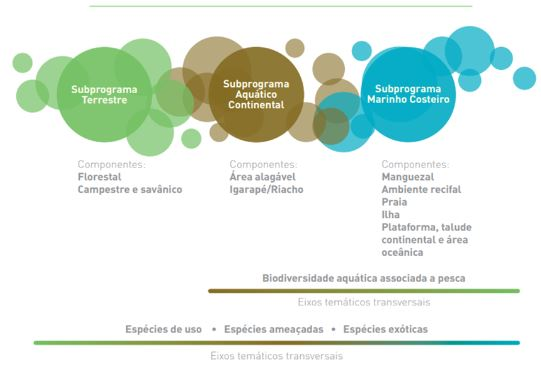
\includegraphics[width=0.7\textwidth,height=\textheight]{imagens/cap01/eixos_tematicos_monitora.JPG}

}

\caption{\label{fig-eixos-tematicos-monitora}Representação esquemática
da estrutura do Programa Monitora.}

\end{figure}%

A busca pela excelência na gestão de dados e informações visa também
potencializar a capacidade analítica, inclusive para subsidiar a
manifestação do instituto e posicionamento da sociedade perante
situações complexas como a implementação de grandes empreendimentos.

O Programa Monitora tem como objetivos:

\begin{itemize}
\item
  gerar informação qualificada para a avaliação continuada da
  efetividade das UCs federais e do Sistema Nacional de Unidades de
  Conservação no cumprimento de seus objetivos de conservação da
  biodiversidade;
\item
  subsidiar, avaliar e acompanhar ``in situ'' projeções de alteração na
  distribuição e locais de ocorrência das espécies em resposta às
  mudanças climáticas e demais vetores de pressão e ameaça, a fim de
  atualizar as medidas de conservação, incluindo o manejo;
\item
  fornecer subsídios para o planejamento do uso sustentável das espécies
  da fauna e flora em unidades de conservação federais;
\item
  fornecer subsídios para a avaliação do estado de conservação da fauna
  e flora brasileira e para implementação das estratégias de conservação
  das espécies ameaçadas de extinção e com dados insuficientes para a
  avaliação (categoria DD); e
\item
  fornecer subsídios para o planejamento e a avaliação de programas de
  controle de espécies exóticas invasoras, especialmente em unidades de
  conservação federais.
\end{itemize}

A gestão do Programa Monitora está a cargo da CGPEQ -- Coordenação Geral
de Pesquisa e Monitoramento da Biodiversidade, mais especificamente da
COMOB -- Coordenação de Monitoramento da Biodiversidade.

As atividades desenvolvidas por essa Coordenação estão previstas no
Decreto nº 10.234, de 11 de fevereiro de 2020, que aprova a Estrutura
Regimental do ICMBio, e estabelece em seu art. 2º, inciso XXVII, entre
as atribuições do instituto: ``desenvolver programa de monitoramento da
biodiversidade para subsidiar a definição e a implementação de ações de
adaptação às mudanças climáticas nas unidades de conservação federais e
a análise da efetividade''.

Para maiores detalhes sobre os subprogramas, componentes e alvos, enfim,
sua estrutura, acesse a
\href{https://www.gov.br/icmbio/pt-br/assuntos/monitoramento/conteudo/Materiais-de-Apoio/estrategia_geral.pdf}{Estratégia
do Programa Nacional de Monitoramento da Biodiversidade -- Programa
Monitora: estrutura (2018)} ou sua
\href{https://www.gov.br/icmbio/pt-br/assuntos/monitoramento/conteudo/estrutura-do-programa-monitora/2b5210461815403eb185f1aceee3b192.pdf}{tabela
resumo}.

\section{Impacto do Programa no desenvolvimento do
conhecimento}\label{impacto-do-programa-no-desenvolvimento-do-conhecimento}

O Programa Monitora até o momento foi responsável pela \ldots..

\section{Os alvos}\label{os-alvos}

A seleção de alvos do componente florestal buscou atender\ldots\ldots..

\bookmarksetup{startatroot}

\chapter{Implementação do Componente
Florestal}\label{implementauxe7uxe3o-do-componente-florestal}

\textbf{O texto precisa ser atualizado.}

\textbf{Jumara Marques de Souza \& Marcelo Lima Reis}

Coordenação de Monitoramento da Biodiversidade - COMOB\\
\emph{Instituto Chico Mendes de Conservação da Biodiversidade --
ICMBio}\\
\emph{Complexo Administrativo EQSW 103/104 s/n}\\
\emph{70670-350 Brasília, DF}

A implementação do Programa Nacional de Monitoramento da Biodiversidade
- Monitora por uma unidade de conservação federal passa por etapas.
Existe um rito ideal a ser seguido, apresentado no documento
\href{https://www.gov.br/icmbio/pt-br/assuntos/monitoramento/conteudo/Materiais-de-Apoio/guiadeimplementaodomonitora16032023.pdf}{Guia
de Implementação do Programa Nacional de Monitoramento da Biodiversidade
(2023)}. Destaca-se nesse processo a necessidade de envolvimento da UC
ou do núcleo de gestão integrada (NGI) e dos demais atores envolvidos,
que são: os Centros Nacionais de Pesquisa e Conservação (CNPCs), a
Coordenação Geral de Pesquisa e Monitoramento da Biodiversidade (CGPEQ)
e a Coordenação de Monitoramento da Biodiversidade (COMOB).

O Monitora está estruturado em subprogramas de acordo com os tipos de
ambientes abrangidos. São três subprogramas: Terrestre, Aquático
Continental e Marinho e Costeiro. Cada subprograma possui diferentes
ecossistemas relacionados, denominados componentes, contendo seus
respectivos alvos de monitoramento, que podem ser grupos taxonômicos,
grupos funcionais, formas de vida, sistemas ecológicos, hábitats ou
ainda processos ecológicos. Os alvos de monitoramento se classificam em
dois tipos: globais (Figura~\ref{fig-alvos-globais}) ou complementares.
Eles estão susceptíveis a sofrerem mudanças ao longo do tempo em
resposta às alterações no meio ambiente e seu potencial de resposta a
essas mudanças é medido por meio do que chamamos de indicadores. Neste
relatório são apresentados os resultados dos protocolos básicos do
componente Florestal.

\begin{figure}[H]

\centering{

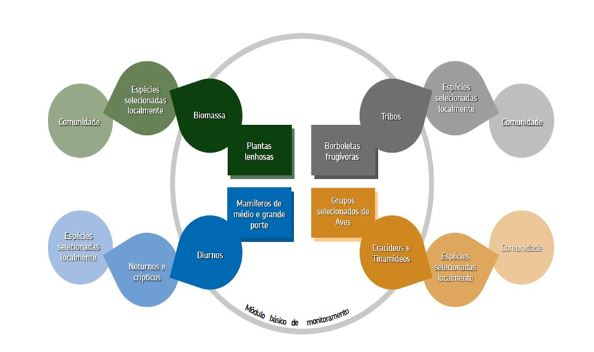
\includegraphics[width=0.7\textwidth,height=\textheight]{imagens/cap02/alvos_globais.JPG}

}

\caption{\label{fig-alvos-globais}Representação esquemática da estrutura
do Programa Monitora (esta figura precisa ser atualizada!).}

\end{figure}%

\section{Métodos}\label{muxe9todos}

\subsection{A Estação Amostral}\label{a-estauxe7uxe3o-amostral}

Os métodos aplicados podem ser encontrados em detalhe no
\href{https://www.gov.br/icmbio/pt-br/assuntos/monitoramento/conteudo/Protocolos-de-Monitoramento/monitoramento_da_biodiversidade_roteiro_metodologico_de_aplicacao_1.pdf}{Monitoramento
da biodiversidade: roteiro metodológico de aplicação (2014)}. Contudo,
apresentamos a seguir um breve resumo dos mesmos.

A aplicação dos protocolos básicos do componente florestal passa ela
implementação das estações amostrais (EAs). Cada EA está relacionada ao
desenho amostral de unidades amostrais (UAs) desenhadas para atender aos
alvos Plantas, Borboletas e Mamíferos e Aves
(Figura~\ref{fig-esquema-estacao-amostral}). E cada UC ou bloco/mosaico
de UC deve implementar ao menos 3 EAs, respeitando a distância mínima
preconizada estas, e realizar a coleta de dados para todos os alvos. A
periodicidade de coleta é anual para Borboletas, Mamíferos e Aves, e a
cada quinquênio para Plantas.

\begin{figure}[H]

\centering{

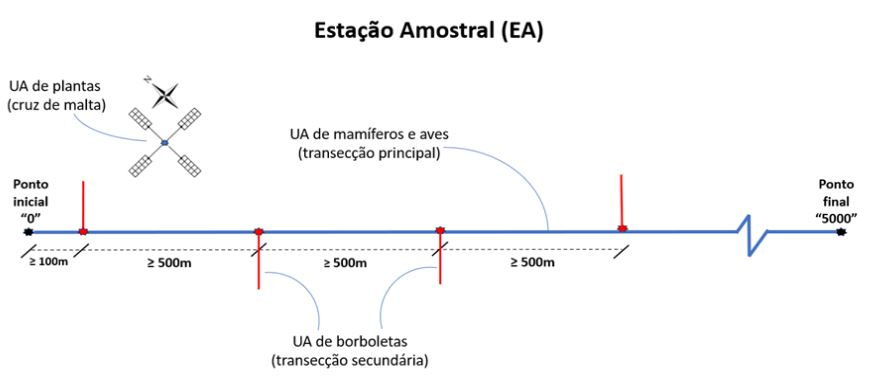
\includegraphics[width=0.7\textwidth,height=\textheight]{imagens/cap02/estacao_amostral.JPG}

}

\caption{\label{fig-esquema-estacao-amostral}Esquema de uma Estação de
Estação Amostral padrão dos alvos globais do Componente Florestal.
Transecção de cinco quilômetros (mamíferos terrestres de médio e grande
porte e aves cinegéticas terrícolas); Transecções secundárias com
baterias de quatro armadilhas de atração por isca (borboletas
frugívoras) e as parcelas permanentes em forma de cruz de malta (plantas
lenhosas).}

\end{figure}%

Para Plantas (Figura~\ref{fig-esquema-unidade-amostral}), a métrica
escolhida para o monitoramento de plantas lenhosas é a biomassa vegetal.
Para isso, é preciso obter os dados de diâmetro e altura estimada das
plantas lenhosas. A coleta de dados ocorre preferencialmente na estação
seca e todos os indivíduos que apresentarem um DAP (diâmetro na altura
do peito = 1,30 m) maior ou igual a 10 cm (circunferência de 31 cm) ou a
30cm do solo (CAS) ≥ 15cm, esse último para plantas localizadas no bioma
Cerrado, são registrados e mensurados.

\begin{figure}[H]

\centering{

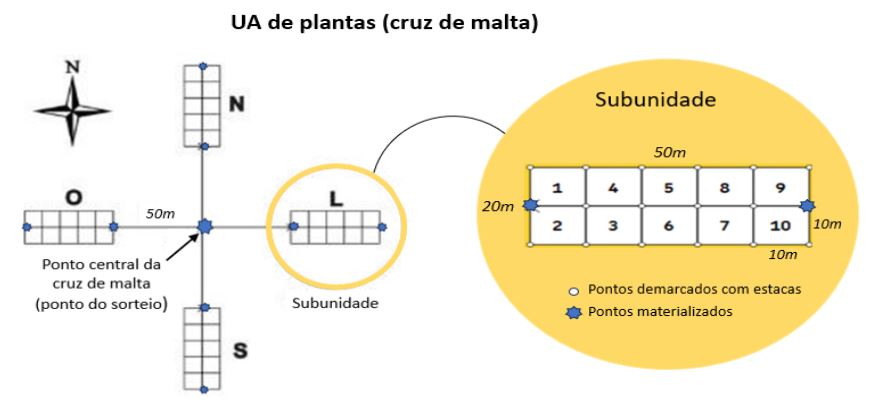
\includegraphics[width=0.7\textwidth,height=\textheight]{imagens/cap02/unidade_amostral.JPG}

}

\caption{\label{fig-esquema-unidade-amostral}Esquema da Unidade Amostral
para monitoramento de Plantas Arbóreas e arborescentes (adaptado de
SFB/Embrapa Florestas, 2012).}

\end{figure}%

A métrica de indicação biológica selecionada para borboletas frugívoras
(Figura~\ref{fig-esquema-borboletas}) é a proporção de indivíduos de
cada tribo realizada com o auxílio de guias de campo. A identificação de
tribos é muito mais simples e viável que a identificação até espécie das
borboletas capturadas. Esse cenário aumenta o potencial de implantação e
manutenção do monitoramento. Neste protocolo são utilizadas armadilhas
do tipo Van Someren-Rydon (VSR) tendo por iscas banana e caldo de cana.
As duas campanhas de coleta de dados se dão preferencialmente ao final
da estação chuvosa, em cada campanha são realizadas ao menos três
vistorias, intercaladas por até 48 horas.

\begin{figure}[H]

\centering{

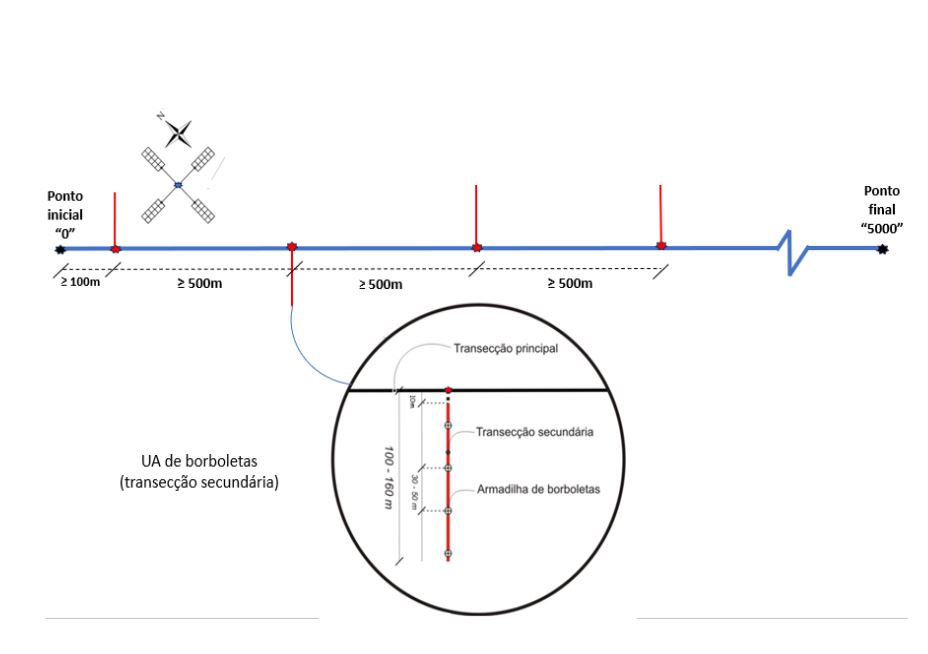
\includegraphics[width=0.7\textwidth,height=\textheight]{imagens/cap02/esquema_unidades_amostrais.JPG}

}

\caption{\label{fig-esquema-borboletas}Esquema das Unidades Amostrais
para monitoramento de borboletas frugívoras.}

\end{figure}%

Para Mamíferos e Aves, a coleta de dados é realizada pelo método de
transecções lineares, quando percorrendo-se as transecções se registra
todos os indivíduos ou grupos das espécies alvo, especialmente sua
localização e distância perpendicular da transecção. As amostragens
ocorrem sempre nas primeiras horas da manhã a uma velocidade média de
1,5km/h. E o esforço mínimo desejado para cada unidade de conservação é
de 150 quilômetros anuais.

\subsection{Unidades de
Conservação}\label{unidades-de-conservauxe7uxe3o}

Três biomas brasileiros, Amazônia, Cerrado e Mata Atlântica, já possuem
unidades de conservação que aderiram em algum grau ao monitoramento de
alvos do componente florestal do Monitora
(Figura~\ref{fig-unidades-conservacao}). A adesão ao componente
Florestal do Programa Monitora significa que as UCs com representantes
capacitados iniciaram a execução do monitoramento, o que incluiu ações
como: reunião com o conselho; capacitação local; solicitação da grade do
Serviço Florestal Brasileiro (GNPA) e escolha locacional de EAs/UAs.
Durante o período de 2013 a 2022, ?? UCs já alcançaram a fase de
operação, ou seja, possuem pelo menos um alvo com coleta de dados de
campo (Tabela~\ref{tbl-numero-ucs}).

\begin{figure}[H]

\centering{

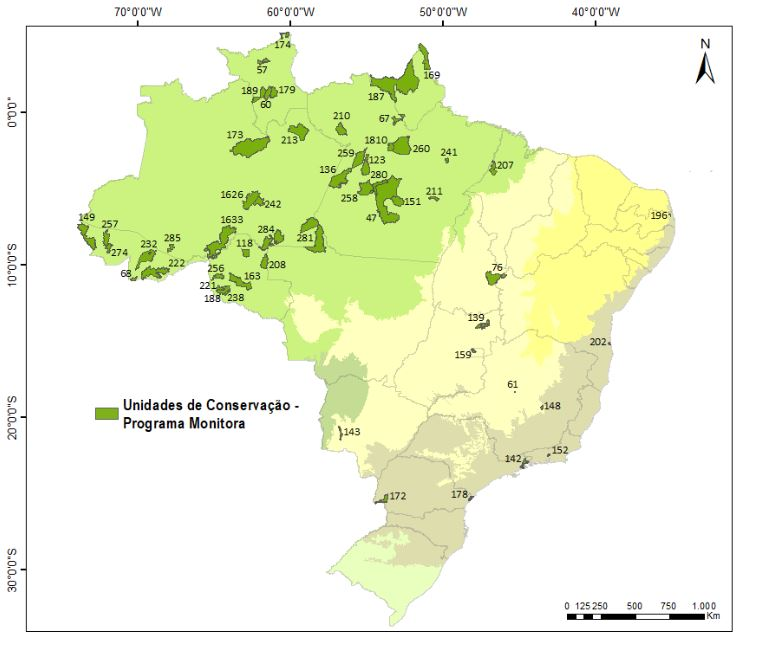
\includegraphics[width=0.7\textwidth,height=\textheight]{imagens/cap02/mapa_unidades.JPG}

}

\caption{\label{fig-unidades-conservacao}Unidades de conservação com
dados validados para análises no período de 2014 a 2022 do componente
Florestal do Programa Monitora. A numeração das UCs corresponde ao seu
cadastro no CNUC.}

\end{figure}%

Considera-se que o monitoramento do componente Florestal está
consolidado quando as UCs possuem pelo menos três EAs implementadas com
todos os alvos de monitoramento com coleta de dados. No final do período
de amostragem de 2022, das ?? UCs em operação, ?? já estavam
consolidadas (??\% -- Tabela~\ref{tbl-numero-ucs}) e, ao todo, o
Programa apresentava ?? EAs e ?? UAs com coleta de dados
(Tabela~\ref{tbl-numero-estacoes}).

\captionsetup{labelsep=none}

\begin{longtable}[t]{lllllllll>{}l}

\caption{\label{tbl-numero-ucs}}

\tabularnewline

\toprule
Etapa & 2014 & 2015 & 2016 & 2017 & 2018 & 2019 & 2020 & 2021 & 2022\\
\midrule
\endfirsthead
\multicolumn{10}{@{}l}{\textit{(continuação)}}\\
\toprule
Etapa & 2014 & 2015 & 2016 & 2017 & 2018 & 2019 & 2020 & 2021 & 2022\\
\midrule
\endhead

\endfoot
\bottomrule
\endlastfoot
Operação  & 16  & 13  & 25  & 30  & 34  & 38  & ??  & ??  & ?? \\
Consolidação  & 0  & 0  & 1  & 6  & 7  & 14  & ??  & ??  & ?? \\*

\end{longtable}

\captionsetup{labelsep=none}

\begin{longtable}[t]{lllllllll>{}l}

\caption{\label{tbl-numero-estacoes}}

\tabularnewline

\toprule
  & 2014 & 2015 & 2016 & 2017 & 2018 & 2019 & 2020 & 2021 & 2022\\
\midrule
\endfirsthead
\multicolumn{10}{@{}l}{\textit{(continuação)}}\\
\toprule
  & 2014 & 2015 & 2016 & 2017 & 2018 & 2019 & 2020 & 2021 & 2022\\
\midrule
\endhead

\endfoot
\bottomrule
\endlastfoot
EA  & 25  & 30  & 51  & 69  & 85  & 95  & ??  & ??  & ?? \\
UA  & 44  & 46  & 86  & 143  & 174  & 239  & ??  & ??  & ?? \\*

\end{longtable}

Das UCs que já alcançaram a fase de operação, 42 UCs são do bioma
Amazônico, seis da Mata Atlântica e seis do Cerrado, e contemplam 18 das
27 unidades federativas do Brasil. Muitas UCs tiveram problemas que
causaram descontinuidade no monitoramento (coleta de dados não realizada
em um ou mais anos) durante o período 2014-2022. Algumas situações se
justificaram pela inadequabilidade dos métodos para o ambiente da UC,
especialmente no Cerrado, outras por problemas de ordem logística,
pessoal ou financeira.

A execução do monitoramento pelas UCs pode ser gradativa, isto é, pode
iniciar com apenas a implantação e coleta de dados de uma EA ou UA e, ao
longo do tempo, chegar na fase de consolidação, mas com a recomendação
de que isso ocorra em até dois anos. Entretanto, verificou-se que a
maioria das UCs, principalmente nos primeiros anos do Programa,
precisaram de mais tempo (de 3 a 4 anos) para atingir a fase de
consolidação. Espera-se que, nos próximos anos, as UCs consigam atingir
a consolidação dentro do período recomendado. É importante ressaltar que
as UCs podem ter mais de três EAs implantadas e outras podem não atingir
essa meta devido a particularidades locais, como algumas unidades do
Cerrado e Mata Atlântica, por suas dimensões, e aquelas que estão
fazendo o monitoramento em ``bloco'' (monitoramento espacialmente
compartilhado).

Esse início gradativo do monitoramento também é observado quando
comparamos o número de UCs, EAs e UAs em operação ao longo do tempo. No
início, a estratégia da maioria das UCs dos biomas Cerrado e Mata
Atlântica foi de priorizar a implementação de apenas uma EA com todas as
respectivas UAs (alvos), enquanto as UCs amazônicas priorizaram as três
EAs, mas não com todos os alvos (trilha ou cruz de malta). A partir de
2016, houve um aumento no esforço de consolidar as EAs com a coleta de
dados de todos os alvos, aumentando consideravelmente o número de UAs
por UC (Figura x, Tabela~\ref{tbl-ucs-componente-florestal}). Portanto,
da mesma forma espera-se que, nos próximos anos, as UCs consigam
aumentar o número de suas EAs e UAs, diminuindo assim a distância entre
a linha do acumulado e do esperado.

\captionsetup{labelsep=none}

\begin{longtable}[t]{lllllllll>{}lll}

\caption{\label{tbl-ucs-componente-florestal}}

\tabularnewline

\toprule
Unidades de Conservação & Nº no mapa (CNUC) & Bioma & 2014 & 2015 & 2016 & 2017 & 2018 & 2019 & 2020 & 2021 & 2022\\
\midrule
\endfirsthead
\multicolumn{12}{@{}l}{\textit{(continuação)}}\\
\toprule
Unidades de Conservação & Nº no mapa (CNUC) & Bioma & 2014 & 2015 & 2016 & 2017 & 2018 & 2019 & 2020 & 2021 & 2022\\
\midrule
\endhead

\endfoot
\bottomrule
\endlastfoot
ESEC de Pirapitinga  & 61  & Cerrado  &  &  &  &  &  &  &  &  & P, B, M/A \\
ESEC Serra Geral do Tocantins  & 76  & Cerrado  & M/A  & P, M/A  &  &  & P  &  &  &  & \\
PARNA da Chapada dos Veadeiros  & 139  & Cerrado  & P, B, M/A  & M/A  & B  & B  & P  &  &  &  & \\
PARNA da Serra da Bodoquena  & 143  & Cerrado  & P, B, M/A  & P, B, M/A  & B, M/A  & B, M/A  & B, M/A  & P, B, M/A  &  &  & M/A \\
PARNA da Serra do Cipó  & 148  & Cerrado  & P, M/A  &  & M/A  & B, M/A  & P, B, M/A  &  &  & B  & B \\
\addlinespace
PARNA de Brasília  & 159  & Cerrado  & P  &  &  & B  & P, B  & B  &  &  & \\
PARNA da Serra da Bocaina  & 142  & Mata Atlântica  & P, M/A  & B, M/A  & B, M/A  &  &  &  &  &  & \\
PARNA da Serra dos Órgãos  & 152  & Mata Atlântica  & P, M/A  & M/A  & P, B, M/A  & B, M/A  &  & P, B, M/A  &  &  & \\
PARNA do Iguaçu  & 172  & Mata Atlântica  &  &  & B, M/A  & B, M/A  & B  & B, M/A  &  & B, M/A  & B, M/A \\
PARNA do Superagui  & 178  & Mata Atlântica  & M/A  & M/A  & P, B, M/A  & P, B  & P, B, M/A  & P, B  &  &  & B \\
\addlinespace
REBIO de Una  & 202  & Mata Atlântica  & M/A  &  &  &  &  &  &  &  & B, M/A \\
REBIO Guaribas  & 196  & Mata Atlântica  &  &  & B, M/A  &  &  &  &  &  & \\
ESEC da Terra do Meio  & 47  & Amazônia  & M/A  &  & P, M/A  & B, M/A  & M/A  &  &  &  & B \\
ESEC de Maracá  & 57  & Amazônia  &  &  &  & P  & B, M/A  & P, B, M/A  &  &  & B, M/A \\
ESEC do Jari  & 67  & Amazônia  &  &  &  &  &  &  &  &  & P, B, M/A \\
\addlinespace
ESEC Niquiá  & 60  & Amazônia  &  &  & P  & B, M/A  & B, M/A  & B, M/A  & B, M/A  & P, B, M/A  & B, M/A \\
ESEC Rio Acre  & 68  & Amazônia  &  &  &  &  &  &  &  & M/A  & B, M/A \\
FLONA do Jamari  & 118  & Amazônia  & P, B, M/A  & B, M/A  & B, M/A  & P, B, M/A  & B, M/A  & M/A  & M/A  & M/A  & B, M/A \\
FLONA do Tapajós  & 123  & Amazônia  &  &  &  &  &  &  &  &  & B, M/A \\
PARNA Campos Amazônicos  & 284  & Amazônia  &  &  &  &  &  & P, M/A  &  & B, M/A  & B, M/A \\
\addlinespace
PARNA da Amazônia  & 136  & Amazônia  &  &  &  & M/A  & P, B, M/A  & B, M/A  & B, M/A  & B, M/A  & B, M/A \\
PARNA da Serra do Divisor  & 149  & Amazônia  &  &  &  &  & P, B, M/A  & P, B, M/A  & P, M/A  & B, M/A  & P, B, M/A \\
PARNA da Serra do Pardo  & 151  & Amazônia  &  &  & M/A  & M/A  & M/A  & M/A  &  &  & P \\
PARNA de Pacaás Novos  & 163  & Amazônia  &  &  &  &  &  & P, B  & B, M/A  & B, M/A  & M/A \\
PARNA do Cabo Orange  & 169  & Amazônia  &  &  & B, M/A  & P, B, M/A  & B, M/A  & B, M/A  & M/A  & B, M/A  & B, M/A \\
\addlinespace
PARNA do Jaú  & 173  & Amazônia  & P  & B, M/A  & B, M/A  & P, B, M/A  & B, M/A  & B, M/A  &  & B, M/A  & P, B, M/A \\
PARNA do Juruena  & 281  & Amazônia  &  &  & M/A  & P, B, M/A  & B, M/A  & B, M/A  & M/A  &  & P, M/A \\
PARNA do Monte Roraima  & 174  & Amazônia  &  &  &  &  &  & P, B, M/A  &  & B, M/A  & B, M/A \\
PARNA Nascentes do Lago Jari  & 1626  & Amazônia  &  &  &  &  &  & P, M/A  &  &  & B, M/A \\
PARNA do Viruá  & 179  & Amazônia  &  &  &  &  & B, M/A  & P, B, M/A  & B, M/A  & B  & B, M/A \\
\addlinespace
PARNA Mapinguari  & 1633  & Amazônia  &  &  &  & P, M/A  & P, B, M/A  & B, M/A  & B, M/A  & P, B, M/A  & P, B, M/A \\
PARNA Montanhas do Tumucumaque  & 187  & Amazônia  & P, M/A  & P, M/A  & P, B, M/A  & B, M/A  & B, M/A  & B, M/A  &  & P, B, M/A  & B, M/A \\
PARNA Serra da Cutia  & 188  & Amazônia  &  &  & P  & B, M/A  & B, M/A  & B, M/A  & B, M/A  & B, M/A  & B, M/A \\
PARNA Serra da Mocidade  & 189  & Amazônia  &  &  & P  & B, M/A  & B, M/A  & B, M/A  & B, M/A  & P, B, M/A  & B, M/A \\
REBIO do Gurupi  & 207  & Amazônia  &  & M/A  & P, B, M/A  & P, B, M/A  & B, M/A  & B, M/A  &  & B, M/A  & B \\
\addlinespace
REBIO do Jaru  & 208  & Amazônia  &  &  & B, M/A  & P, B, M/A  & B, M/A  & B, M/A  & B, M/A  & B, M/A  & P, B, M/A \\
REBIO do Tapirapé  & ´211  & Amazônia  &  &  & P, B, M/A  & P, B, M/A  & B, M/A  & B, M/A  &  & B, M/A  & B, M/A \\
REBIO do Uatumã  & 213  & Amazônia  & P, B, M/A  & B, M/A  & B, M/A  & P, B, M/A  & B, M/A  & B, M/A  & B, M/A  & B, M/A  & \\
RESEX Arapixi  & 285  & Amazônia  &  &  &  &  &  & P, B, M/A  & M/A  & B, M/A  & B, M/A \\
RESEX Barreiro das Antas  & 221  & Amazônia  &  &  &  & P, M/A  & P, B, M/A  & B, M/A  & B, M/A  & B, M/A  & B, M/A \\
\addlinespace
RESEX Chico Mendes  & 222  & Amazônia  &  &  &  &  & B, M/A  & B, M/A  &  &  & \\
RESEX do Alto Tarauacá  & 274  & Amazônia  &  &  &  & B, M/A  & P, B, M/A  & B, M/A  & M/A  & B, M/A  & B, M/A \\
RESEX do Cazumbá-Iracema  & 232  & Amazônia  & P, M/A  & M/A  & B, M/A  & P, B, M/A  & B, M/A  & P, B, M/A  & M/A  & B, M/A  & B, M/A \\
RESEX do Lago do Capanã Grande  & 242  & Amazônia  &  &  &  &  &  &  &  & B, M/A  & B, M/A \\
RESEX do Rio Cautário  & 238  & Amazônia  &  &  &  &  &  & B, M/A  &  & B, M/A  & B, M/A \\
\addlinespace
RESEX Ipaú-Anilzinho  & 241  & Amazônia  &  &  &  &  &  & P, B, M/A  & B, M/A  & B, M/A  & B, M/A \\
 &  &  &  &  &  &  &  &  &  &  \vphantom{2} & \\
RESEX Renascer  & 1810  & Amazônia  &  &  &  &  & P, B, M/A  & B  & M/A  & B, M/A  & \\
RESEX Rio Iriri  & 280  & Amazônia  &  &  &  &  &  &  &  &  & M/A \\
RESEX Rio Ouro Preto  & 256  & Amazônia  &  &  &  & P, B, M/A  & B, M/A  & B, M/A  & M/A  & B, M/A  & B, M/A \\
\addlinespace
RESEX Riozinho da Liberdade  & 257  & Amazônia  &  &  &  &  &  &  & P, B, M/A  & B, M/A  & P, B, M/A \\
 &  &  &  &  &  &  &  &  &  &  \vphantom{1} & \\
RESEX Riozinho do Anfrízio  & 258  & Amazônia  &  &  & M/A  & M/A  & M/A  & B, M/A  &  &  & B, M/A \\
RESEX Tapajós-Arapiuns  & 259  & Amazônia  & M/A  & B, M/A  & B, M/A  & B, M/A  & P, B, M/A  & B, M/A  & M/A  & B, M/A  & B, M/A \\
REBIO do Rio Trombetas  & 210  & Amazônia  &  &  &  &  &  & M/A  &  &  & \\
\addlinespace
 &  &  &  &  &  &  &  &  &  &  & \\
RESEX Verde Para Sempre  & 260  & Amazônia  &  &  &  &  &  &  &  &  & P, B, M/A \\*

\end{longtable}

Para detalhes da implementação dos diferentes protocolos por UC ao longo
dos anos veja Apêndice B (verificar com os pontos focais a viabilidade
de apresentação desses dados!).

\section{Resultados da
implementação}\label{resultados-da-implementauxe7uxe3o}

Nos capítulos seguintes (3, 4 e 5) são apresentados resultados gerais
obtidos com a implementação do Componente Florestal do Programa Monitora
no período de 2014 a 2022, organizados por alvo e segmentados por
biomas, além de informações sobre um recorte de espécies ameaçadas.
Quando pertinente, resultados parciais e particularidades de algumas
unidades de conservação foram também destacadas. Por sua vez, tendo em
vista o caráter geral desse relatório, informações complementares e
resultados específicos mais completos por alvo para cada unidade de
conservação serão apresentados futuramente numa
\href{https://argofix.shinyapps.io/teste_shp/}{plataforma \emph{on-line}
interativa} atualmente em desenvolvimento. No capítulo 6 são discutidos
alguns padrões de respostas congruentes entre os alvos e suas potenciais
correlações.

\bookmarksetup{startatroot}

\chapter{Plantas}\label{plantas}

\textbf{Alexandre Bonesso Sampaio\textsuperscript{1}, Bruno Lenhaverde
Sandy\textsuperscript{2}, Jumara Marques Sousa\textsuperscript{2} \&
Rafaela Campostrini Forzza\textsuperscript{3-4}}

\begin{enumerate}
\def\labelenumi{\arabic{enumi}.}
\item
  Centro Nacional de Pesquisa e Conservação da Biodiversidade do Cerrado
  e Restauração Ecológica - CBC*\\
  \emph{Instituto Chico Mendes de Conservação da Biodiversidade --
  ICMBio}\\
  \emph{Parque Nacional de Brasília}\\
  \emph{Via Epia, BR-450, Km 8,5}\\
  \emph{70635-800 Brasília, DF}
\item
  Coordenação de Monitoramento da Biodiversidade - COMOB\\
  \emph{Instituto Chico Mendes de Conservação da Biodiversidade --
  ICMBio}\\
  \emph{Complexo Administrativo EQSW 103/104 s/n}\\
  \emph{70670-350 Brasília, DF}
\item
  Jardim Botânico do Rio de Janeiro -- JBRJ\\
  \emph{Rua Jardim Botânico, 1008}\\
  \emph{Jardim Botânico}\\
  \emph{22460-030 Rio de Janeiro, RJ}
\item
  Parque Nacional do Descobrimento\\
  \emph{Instituto Chico Mendes de Conservação da Biodiversidade -
  ICMBio}\\
  \emph{Cumuruxatiba}\\
  \emph{45980-000 Prado, BA}
\end{enumerate}

\section{Estado da implementação}\label{estado-da-implementauxe7uxe3o}

Para o período de 2014 a 2022 foram registradas 45 UCs federias em
operação, isto é, com amostragens de plantas arbóreas e arborescentes
nas cruzes de malta. Sendo 36 na Amazônia, seis no Cerrado e três na
Mata Atlântica. Destas, 44 enviaram dados a tempo de compor este
relatório.

Das 45 UC federais com coleta de dados de plantas, 26 (58\%) já estão
consolidadas, isto é, possuem pelo menos três unidades amostrais (cruzes
de malta) em operação. No total, o Programa já possui 104 UAs (cruzes da
malta) de plantas em operação.

Oito UCs já fizeram as remedições de 5 anos: Esec Niquiá, Parna Serra da
Mocidade, Parna do Jaú, Parna do Juruena, Rebio do Jaru, Parna Montanhas
do Tumucumaque, Parna do Cabo Orange e Rebio do Uatumã, sendo que as
duas últimas ainda não entregaram os dados à COMOB. Quatro UCs estão com
as coletas atrasadas em 1 ano (Flona Jamari, Rebio do Tapirapé, Rebio do
Gurupi e Resex Ouro Preto) e três estão com atrasos maiores,
consideradas como ``paradas ou interrompidas'' (Esec da Terra do Meio,
Parna Serra da Cutia e Parna da Serra da Bocaina). Quatro UCs entraram
em operação em 2022 (Esec Pirapitinga, Esec Jari, Resex Verde para
Sempre e a Flona Carajás).

\section{Resultados}\label{resultados}

\subsection{Estrutura}\label{estrutura}

Nesse quinquênio, foram monitoradas ?? plantas, especificamente ??
árvores, ?? palmeiras, ?? cipós e ?? pteridófitas arborescentes; ??
indivíduos não receberam categorização em campo (Figura x).

As análises dos dados dos quinquênios compreendidos no período de
2014-2022 consistiram de avaliações descritivas sobre a estrutura das
vegetações amostradas com ênfase na altura, circunferência, área basal e
biomassa.

Entre as unidades de conservação monitoradas no período de 2014 a 2022,
destacam-se duas UCs localizadas no Cerrado com o maior número de
árvores amostradas por área em comparação às demais UCs, as quais são o
PARNA de Brasília (ano 2018 - 3.185 ± 302,93 ind./ha e ano 2014 - 2537,5
± 995,67 ind./ha) e a ESEC Serra Geral do Tocantins (ano 2015 - 1005 ±
135,28 ind./ha). Estas foram as únicas UCs amostradas a utilizarem como
critério de inclusão o CAS ≥ 15 cm, sendo, portanto, um critério menos
restritivo do que aquele utilizado na Amazônia e Mata Atlântica (CAP ≥
31 cm). Na Amazônia, as maiores densidades médias foram registradas na
ESEC Niquiá (1002,5 ± 159,87 - ano 2016) e no PARNA do Jaú (755 ± 79,37
ind./ ha -- ano 2014). Na Mata Atlântica, destacam-se os PARNAs do
Superagui (965 ± 561,45 ind./ha -- ano 2018) e da Serra da Bocaina
(866,7 ± 445,94 ind./ ha -- ano 2014) com as maiores densidades (Anexo
Plantas)

Com exceção da ESEC Niquiá e do PARNA do Jaú, as UCs amostradas na
Amazônia apresentaram baixa densidade de indivíduos quando comparadas
com as demais UCs amostradas; em contrapartida, as plantas da maior
parte dessas UCs apresentaram as maiores circunferências registradas e
ocupam uma maior área no espaço, como indicam os elevados valores de
área basal -- estimativa da área de superfície do solo ocupada por uma
planta. No PARNA Montanhas do Tumucumaque foram registrados, em 2015, os
maiores valores de circunferência e área basal média, respectivamente:
83,14 ± 93,88 cm e 63,65 ±131,49 m²/ha; assim como na ESEC da Terra do
Meio, em 2016: 75,2 ± 87,79 cm; 54,07 ± 120,52 m²/ha. Os menores valores
de circunferência e área basal para a Amazônia foram registrados nas
RESEX do Cazumbá-Iracema, em 2014 (59,85 ± 36,75 cm e 11,13 ± 12,41
m²/ha) e Barreiro das Antas, em 2018 (54,12 ± 23,89 cm e 13,13 ± 8,59
m²/ha).

Entre as UCs monitoradas na Mata Atlântica, os maiores valores de
circunferência e área basal média foram registrados no PARNA da Serra
dos Órgãos em 2014 (68,48 ± 45,44 cm e 43,48 ± 38,80 m²/ha) e os
menores, em 2016, no PARNA do Superagui (60,51 ± 36,93 cm e 19,37 ±
17,43 m²/ha). Para as UCs do bioma Cerrado, nas quais o CAP foi
utilizado para a realização das análises, os valores de circunferência e
área basal média tenderam a ser menores do que aqueles registrados na
Mata Atlântica e Amazônia, como no PARNA da Serra da Bodoquena, em 2014
(59,71 ± 32,45 cm e 25,15± 16,02 m²/ha) e no PARNA da Serra do Cipó, em
2014 (57,57 ± 33,86 cm e 12,25 ± 10,77 m²/ha). Para as demais UCs do
Cerrado utilizou-se o CAS nas análises, sendo os menores valores de
circunferência e área basal média registrados no PARNA de Brasília, em
2014 (25,4 ± 11,68 cm e 18,56 ± 8,12 m²/ha).

O valor de cobertura, dado pelo quociente da área basal média pelo
número total de indivíduos, também corrobora a relação inversa existente
entre densidade e circunferência. Assim como a área basal, a Amazônia
concentra elevados valores de cobertura, seguida pela Mata Atlântica e
Cerrado. Os maiores valores de cobertura foram encontrados no PARNA
Montanhas do Tumucumaque em 2015 (0,125) e 2017 (0,114) e os menores, no
PARNA de Brasília em 2014 e 2018 (0,006) (Anexo Plantas).

Os indivíduos amostrados no período entre 2014 e 2022 foram organizados
em histogramas conforme a frequência nas classes de circunferência. Pela
análise gráfica é possível observar que a maioria das UCs apresentam uma
distribuição esperada para vegetações bem preservadas. Isto é, os dados
das UCs se ajustam a uma curva exponencial, apresentando uma
distribuição em formato de ``J'' invertido (ver plataforma online).

Em relação à altura, as plantas mais altas foram registradas nas UCs da
Amazônia, entre elas se destaca o PARNA Montanhas do Tumucumaque, com o
registro em 2017 do maior indivíduo amostrado: 64 m (Figura x). Na Mata
Atlântica, a maior altura registrada foi 30 m (PARNA da Serra dos
Órgãos) e no Cerrado, 55 m, no PARNA da Serra da Bodoquena (Figura x).
Os dados de altura das plantas correspondem a estimativas e devem ser
analisados com cautela. Esse foi um dos motivos que nos levou a excluir
alguns dados de altura de alguns indivíduos em UCs do Cerrado nessa
análise, pois algumas plantas cuja espécie era conhecida apresentaram
valores muito acima do esperado e possivelmente são erros de amostragem.

\begin{figure}[H]

\centering{

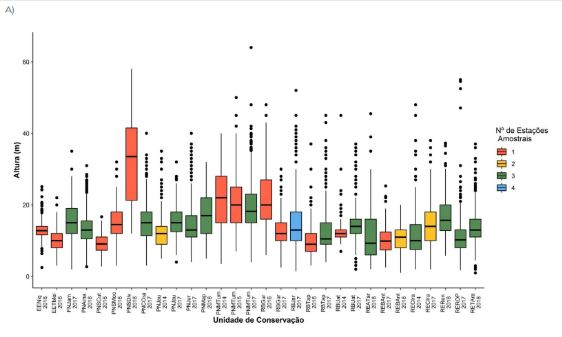
\includegraphics[width=0.7\textwidth,height=\textheight]{imagens/cap03/pl_boxplot1.JPG}

}

\caption{\label{fig-boxplot1}Boxplot 1.}

\end{figure}%

\begin{figure}[H]

\centering{

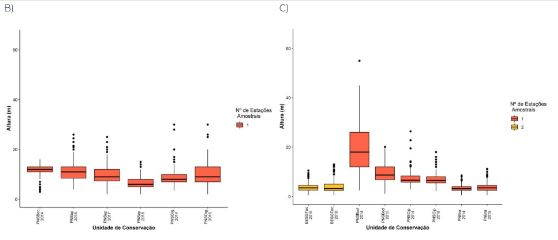
\includegraphics[width=0.7\textwidth,height=\textheight]{imagens/cap03/pl_boxplot2.JPG}

}

\caption{\label{fig-boxplot2}Boxplot 2.}

\end{figure}%

\subsection{Biomassa}\label{biomassa}

Como o protocolo básico de plantas não prevê a identificação dos
indivíduos amostrados, foram escolhidas, com auxílio de especialistas,
equações gerais para estimar a biomassa das ``árvores em pé'' dos três
biomas amostrados. A estimativa de biomassa de plantas com equações
gerais é menos precisa do que aquela realizada com equações específicas
para espécie; no entanto, representa um bom indicativo do papel desses
organismos no ciclo do carbono.

Para o bioma Amazônia foram utilizadas duas equações, conforme {[}1{]},
para estimar a biomassa fresca, dada em quilograma (kg):

\begin{enumerate}
\def\labelenumi{(\arabic{enumi})}
\item
  Biomassa = exp (-1,754 + 2,665 Ln(DAP)) para plantas com 5 ≤ DAP
  \textless20 cm; e,
\item
  Biomassa = exp (-0,151 + 2,170 Ln(DAP)) para plantas com DAP ≥ 20 cm;
  onde, DAP = diâmetro à altura do peito (cm).
\end{enumerate}

A equação utilizada para estimar a biomassa (kg) na Mata Atlântica foi
adaptada de {[}2{]}:

\begin{enumerate}
\def\labelenumi{(\arabic{enumi})}
\setcounter{enumi}{2}
\tightlist
\item
  Biomassa = exp (-10,6409194002 + 2,1533324963 Ln(DAP) + 0,8248143766
  Ln(H)) 1000; onde, H = altura (m).
\end{enumerate}

Foi utilizada a equação de {[}3{]} para áreas de cerrado \emph{sensu
stricto}:

\begin{enumerate}
\def\labelenumi{(\arabic{enumi})}
\setcounter{enumi}{3}
\tightlist
\item
  Biomassa = -0,49129 + 0,02912(DAP²)H
\end{enumerate}

Os valores obtidos pelas fórmulas citadas foram convertidos para
toneladas (t), por conveniência, para melhor visualização e comparação
dos dados. Entre as UCs monitoradas, aquelas localizadas no bioma
Amazônia apresentaram os maiores valores de biomassa, os quais variaram
de 611,82 t (PARNA Montanhas do Tumucumaque -- ano 2015) a 74,74 t
(PARNA Mapinguari -- ano 2018) (Anexo Plantas). Os menores valores de
biomassa foram encontrados nas UCs de Cerrado, a exemplo da EA-2 da ESEC
Serra Geral do Tocantins, em 2015, que teve a menor estimativa de
biomassa de todas as UCs monitoradas: 4,22 t. A estimativa da biomassa
para a Mata Atlântica apresentou valores intermediários entre aqueles
calculados para Amazônia e Cerrado, variando de 50,53 (PARNA da Serra
dos Órgãos -- ano 2014) a 16,24 t (PARNA do Superagui -- ano 2018).

O PARNA da Serra da Bodoquena é a única unidade de conservação
monitorada no bioma Cerrado em que as unidades amostrais (cruzes de
malta) estão implantadas em uma floresta estacional. As cruzes das
demais UCs estão em uma vegetação do tipo cerrado sensu stricto. Por
conta disso, os indivíduos do PARNA da Serra da Bodoquena apresentam uma
maior amplitude de altura (de 1,1 a 55 m) (Figura x) e circunferência
(31 a 263 cm) em comparação às demais UCs monitoradas no Cerrado.

O PARNA da Serra do Cipó é um caso especial. Embora a vegetação da
unidade amostral localizada no PARNA seja categorizada como cerrado
sensu stricto, essa área sofre influência de uma mata de galeria
localizada nas proximidades, o que reflete nos elevados valores de
cobertura, os maiores registrados para as UCs monitoradas no Cerrado no
período entre 2014 e 2018. O PARNA da Serra do Cipó apresentou valores
elevados de biomassa 19,29 e 18,27 t.

Ao analisar as variáveis medidas pelo protocolo de plantas e sua
variação ao longo do tempo, observamos que as áreas estudadas apresentam
bom estado de conservação, que parece estar se mantendo. Porém, essa é
uma impressão prematura, pois poucas UCs tiveram mais de uma amostragem
ao longo do tempo. Assim, para que se tenha confiabilidade nessa
informação são necessárias mais medidas das parcelas implantadas.

\subsection{Relatório do sistema}\label{relatuxf3rio-do-sistema}

O relatório do sistema é uma versão condensada do relatório 2, agrupando
as UCs por bioma -- sendo que a Amazônia pode ser apresentada em dois
recortes: calha norte e calha sul. Avaliar se outros alvos estão usando
outros recortes, para fazer semelhante.

Recortes:

Amazonia -calha norte

Amazonia -- sul

Mata atlântica

Cerrado (checar se tem t1 p cerrado)

Para cada um dos recortes, serão apresentados 4 figuras:

Índice de Liocourt em T0 e T1 -- gráfico tipo um boxplot, só que a
representação gráfica é tipo uma bolha mais larga onde tem mais pontos,
mais estreita onde tem menos. -- \emph{violin plot} -- ver figura
abaixo.

\begin{figure}[H]

\centering{

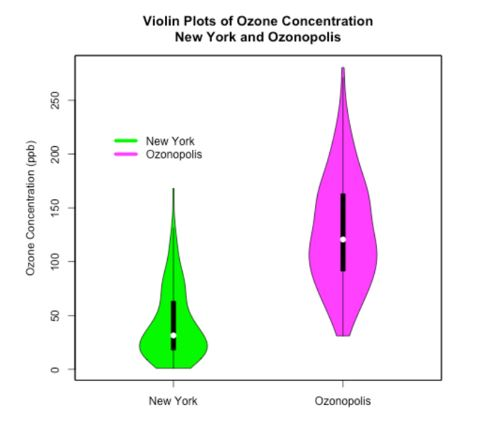
\includegraphics[width=0.7\textwidth,height=\textheight]{imagens/cap03/pl_violino1.JPG}

}

\caption{\label{fig-violino1}Boxplot 2.}

\end{figure}%

E outra figura mostrando quantas ucs de moveram em cada direção
considerando o delta Liocourt -- tipo um gráfico pirâmide -- ver figura
abaixo.

Biomassa em T0 e T1 -- violin plot

Figura semelhante a b para biomassa.

\subsection{Destaques}\label{destaques}

\subsection{Contraste entre o Inventário Florestal Nacional e os dados
do protocolo básico de plantas do componente
florestal}\label{contraste-entre-o-inventuxe1rio-florestal-nacional-e-os-dados-do-protocolo-buxe1sico-de-plantas-do-componente-florestal}

\emph{There are many variations of passages of Lorem Ipsum available,
but the majority have suffered alteration in some form, by injected
humour, or randomised words which don't look even slightly believable.
If you are going to use a passage of Lorem Ipsum, you need to be sure
there isn't anything embarrassing hidden in the middle of text. All the
Lorem Ipsum generators on the Internet tend to repeat predefined chunks
as necessary, making this the first true generator on the Internet. It
uses a dictionary of over 200 Latin words, combined with a handful of
model sentence structures, to generate Lorem Ipsum which looks
reasonable. The generated Lorem Ipsum is therefore always free from
repetition, injected humour, or non-characteristic words etc.}

\section{Discussão}\label{discussuxe3o}

\emph{There are many variations of passages of Lorem Ipsum available,
but the majority have suffered alteration in some form, by injected
humour, or randomised words which don't look even slightly believable.
If you are going to use a passage of Lorem Ipsum, you need to be sure
there isn't anything embarrassing hidden in the middle of text. All the
Lorem Ipsum generators on the Internet tend to repeat predefined chunks
as necessary, making this the first true generator on the Internet. It
uses a dictionary of over 200 Latin words, combined with a handful of
model sentence structures, to generate Lorem Ipsum which looks
reasonable. The generated Lorem Ipsum is therefore always free from
repetition, injected humour, or non-characteristic words etc.}

\section{Recomendações}\label{recomendauxe7uxf5es}

\emph{There are many variations of passages of Lorem Ipsum available,
but the majority have suffered alteration in some form, by injected
humour, or randomised words which don't look even slightly believable.
If you are going to use a passage of Lorem Ipsum, you need to be sure
there isn't anything embarrassing hidden in the middle of text. All the
Lorem Ipsum generators on the Internet tend to repeat predefined chunks
as necessary, making this the first true generator on the Internet. It
uses a dictionary of over 200 Latin words, combined with a handful of
model sentence structures, to generate Lorem Ipsum which looks
reasonable. The generated Lorem Ipsum is therefore always free from
repetition, injected humour, or non-characteristic words etc.}

\bookmarksetup{startatroot}

\chapter{Borboletas}\label{borboletas}

\textbf{Isabela Oliveira \& Onildo João Marini Filho}

Centro Nacional de Pesquisa e Conservação da Biodiversidade do Cerrado e
Restauração Ecológica - CBC\\
\emph{Instituto Chico Mendes de Conservação da Biodiversidade --
ICMBio}\\
\emph{Parque Nacional de Brasília}\\
\emph{Via Epia, BR-450, Km 8,5}\\
\emph{70635-800 Brasília, DF}

A variação da frequência relativa de ocorrência das tribos de borboletas
frugívoras ao longo dos anos vem sendo utilizada como indicador de
alteração ambiental para insetos. Esse indicador está relacionado tanto
a alterações na vegetação ({[}4{]}; {[}5{]}) quanto àquelas menos
perceptíveis, como a qualidade do ar (especialmente a presença de
agrotóxicos) ({[}6{]}, {[}7{]}) e do clima (temperatura, umidade e
extremos climáticos) ({[}8{]}).

A análise que vem sendo utilizada considera a existência de um gradiente
de associação entre as tribos de borboletas frugívoras e as formações
florestais mais ou menos abertos. O conceito adotado pelo grupo de
especialistas em borboletas é de que as 13 tribos estão relacionadas aos
seguintes tipos de ambientes:

\begin{itemize}
\item
  tribos típicas de ambientes florestais fechados/conservados:
  Brassolini, Haeterini e Morphini. Essas tribos diminuem
  consistentemente a abundância relativa em situações de perturbações da
  floresta;
\item
  tribos associadas a ambientes florestais alterados (que causam a
  abertura do dossel da floresta) e/ou favorecidas por perturbações:
  Ageroniini, Callicorini e Biblidini. Essas tribos aumentam
  consistentemente em abundância com perturbações na floresta;
\item
  tribos sem associação clara com ambientes florestais ou sem tendência
  definida: Preponini, Melanitini, Anaeini, Epicaliini, Epiphilini,
  Coeini e Satyrini. Essas tribos podem aumentar ou diminuir com
  perturbações da floresta, como abertura de clareiras ou eventuais
  alterações no dossel.
\end{itemize}

\section{Estado da implementação}\label{estado-da-implementauxe7uxe3o-1}

Para o período de 2014 a 2022 foram registradas 50 UCs federias, 134 EAs
e 536 UAs (transecções com quatro armadilhas de atração por iscas) em
operação, isto é, com amostragens do alvo borboletas frugívoras. Destas,
uma UC do bioma Cerrado (Parna da Chapada dos Veadeiros) interrompeu a
amostragens, pois as UAs estavam em ambientes savânicos e deverá voltar
ao Monitora Florestal com amostragens de UAs em ambientes de mata de
galeria. No caso do Parna de Brasília, ainda estão sendo realizadas as
amostragens em ambiente savânico, mas que deverão ser considerados como
do componente Campestre e Savânico. A planilha oficial validada com os
dados brutos do alvo global Borboletas frugívoras - Componente
Florestal, atualmente possui 82.349 registros (linhas).

Apenas duas UCs (Parna de Pacaás Novos e Rebio do Uatumã) coletaram os
dados de 2022, mas não enviaram à COMOB a tempo de compor este relatório
e o Parna de Brasília realizou a campanha de 2022 no ODK, com os dados
inseridos no \emph{i-naturalist} e em planilha \emph{google drive},
portanto, não disponibilizados nesta planilha, sendo necessária a
conversão para o formato .xls com a mesma configuração da planilha
padronizada.

Das 50 UCs federais com coleta de dados de borboletas frugívoras, 33
(66\%) já estão consolidadas, isto é, possuem pelo menos três unidades
amostrais (transecções lineares) em operação. Três UCs retomaram as
amostragens em 2022 (Esec Maracá, Esec Terra do Meio/Iriri e o Parna do
Superagui), seis UCs (Parna do Juruena, Resex Chico Mendes, Parna da
Bocaina, Parna da Serra dos Órgãos, Parna da Bodoquena e Rebio Guaribas)
são consideradas como paradas ou interrompidas (mais de dois anos
consecutivos sem amostragem) e apenas uma UC (Resex Renascer) parou a
amostragem em 2022.

Em 2022, a amostragem de borboletas frugívoras foi realizada em 40 das
50 UCs que aderiram ao Programa Monitora, nos três biomas florestais
(Tabela x). O ano de 2022 teve 21 UCs a mais do que 2021, e os números
indicam aumento de 26\% na quantidade de Estações Amostrais (EAs)
implementadas (Figura~\ref{fig-evolucao-implementacao}). Todas as oito
novas UCs que aderiram ao Monitora e iniciaram a amostragem de
borboletas são amazônicas e apoiadas pelo Programa ARPA. As ? UCs
apoiadas pelo ARPA são as que apresentam os melhores índices de
implementação dos protocolos de borboletas, sendo que ?? delas (??\%) já
estão consolidadas, com pelo menos três UAs sendo amostradas.

\begin{figure}[H]

\centering{

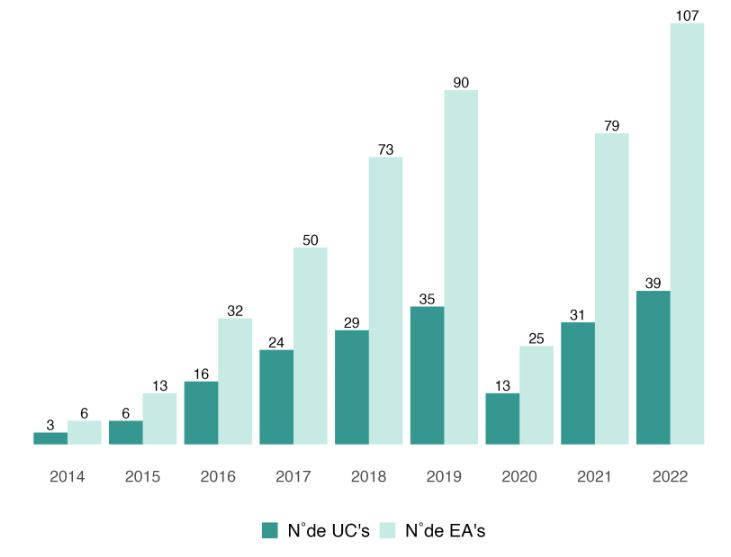
\includegraphics[width=0.7\textwidth,height=\textheight]{imagens/cap04/bo_evolucao_implementacao.JPG}

}

\caption{\label{fig-evolucao-implementacao}Evolução da implementação das
amostragens de borboletas em todas as UCs participantes do Programa
Monitora.}

\end{figure}%

O esforço amostral vem aumentando quase linearmente a uma taxa de
15-20\%, ao se comparar com os anos subsequentes desde o início da
implementação do Programa Monitora. O número de registros aumentou
desproporcionalmente ao esforço em 2016, aparentemente devido a fatores
climáticos. O número acumulado de registros de borboletas amostradas em
nível de tribo (protocolo básico) totalizou ?? indivíduos
(Figura~\ref{fig-esforco-amostral}).

\begin{figure}[H]

\centering{

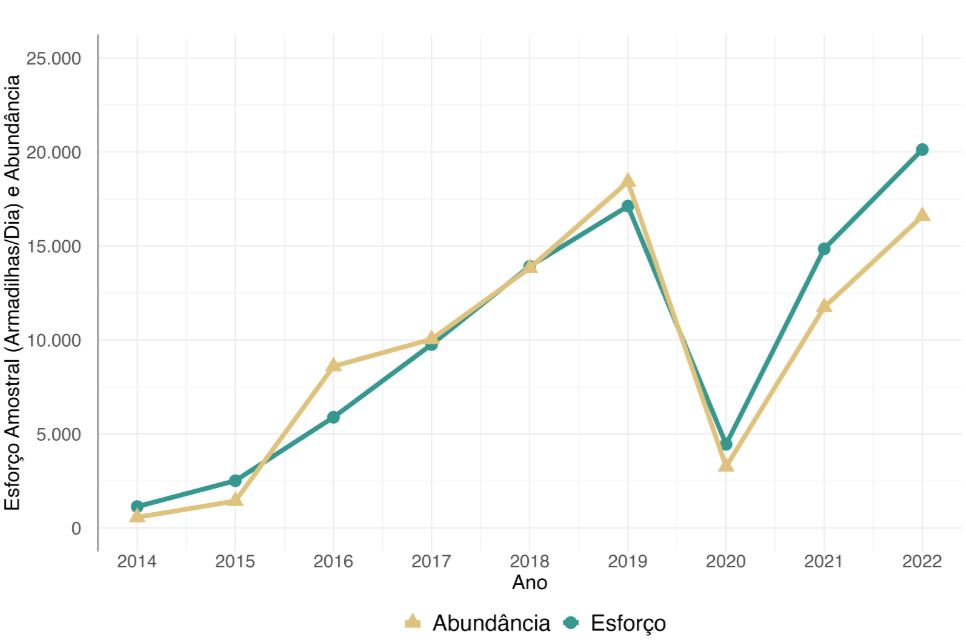
\includegraphics[width=0.7\textwidth,height=\textheight]{imagens/cap04/bo_esforco.JPG}

}

\caption{\label{fig-esforco-amostral}Variação no número de registros de
borboletas frugívoras e esforço amostral (dias*armadilhas) somada para
todas as UCs participantes do Programa Monitora.}

\end{figure}%

\subsection{Considerações sobre as amostragens na Mata
Atlântica}\label{considerauxe7uxf5es-sobre-as-amostragens-na-mata-atluxe2ntica}

O padrão de baixos números de indivíduos capturados vem sendo observado
para todas as UCs da Serra do Mar e baixada litorânea (Parnas da Serra
dos Órgãos, da Serra da Bocaina e do Superagui). Ainda não sabemos o
motivo de o método não estar rendendo os mesmos resultados que são
observados para outras UCs em outros ambientes. Esse padrão talvez
esteja indicando que o período ideal de coleta tenha que ser deslocado
para o final da estação seca, devido ao padrão bimodal de ocorrência de
borboletas nesses ambientes ({[}5{]}; {[}9{]}) bem como em outras
regiões montanhosas da Mata Atlântica.

Considerando isso, o grupo de análise de dados sugere que sejam
exploradas outras possibilidades de desenho amostral para essa região
que possam ajudar a solucionar o problema, gerando maiores volumes de
dados. Sugerimos implementar experimentalmente uma coleta adicional no
final da estação seca nas UCs onde a logística permitir. Essa sugestão
pode ser estendida para matas paludosas e sazonalmente alagadas. Outra
questão importante a ser considerada na escolha do local de instalação
das unidades amostrais é evitar a face sul das montanhas para a
colocação das estações amostrais nessas UCs. Pode-se também avaliar a
possibilidade de amostrar no dossel das matas paludosas e sazonalmente
alagadas, uma vez que a comunidade de sub-bosque de matas muito
sombreadas e alagadas frequentemente se mostra muito incipiente
({[}10{]}; {[}11{]}).

\section{Resultados}\label{resultados-1}

\subsection{Amazônia}\label{amazuxf4nia}

\subsubsection{Síntese por região
climática}\label{suxedntese-por-regiuxe3o-climuxe1tica}

O objetivo dessa seção é buscar análises integrativas que gerem padrões
regionais ou geográficos que possam mostrar alterações na biodiversidade
em escala ampla. Neste período inicial do Programa Monitora, serão
estabelecidos os padrões normais para cada UC e, possivelmente, para
cada região. A primeira tentativa que estamos adotando é a geração das
proporções normais de abundância relativa de tribos por região climática
conforme apresentado a seguir.

Considerando que ainda não temos dados populacionais para borboletas,
uma vez que poucas UCs iniciaram a adoção do protocolo avançado, ainda
estamos incapacitados de gerar tendências nesse nível. Uma dessas
tendências desejadas seria o cálculo de um índice de abundância sobre
esforço amostral para cada população monitorada -- igual ou similar ao
Índice Planeta Vivo ({[}12{]}). Para que isso seja possível,
necessitamos de dados populacionais coletados em eventos anuais para
cada uma das espécies em cada unidade de conservação ou estação amostral
para anos consecutivos. Com esse tipo de dado, obteríamos tendências de
aumento ou diminuição de populações em EAs, UCs, ou regiões climáticas
({[}13{]}).

Mesmo não tendo acesso a dados populacionais, estamos avaliando a
possibilidade de uso de um índice no nível de tribos para servir de base
para futuras aplicações ao Programa Monitora. Uma proposta será
apresentada adiante.

As datas de amostragem propostas para borboletas frugívoras na Amazônia
seguem a mesma lógica aplicada para as regiões Central e Sudeste do
Brasil, onde temos alta abundância populacional e maior diversidade de
espécies de borboletas frugívoras no final do período de chuvas intensas
({[}14{]}). A proposta de regiões amazônicas apresentada a seguir se
baseia na caracterização climática associada ao padrão de chuvas em toda
a Amazônia (Figura~\ref{fig-regioes-climaticas}, reproduzida de
{[}15{]}). A partir da determinação dos regimes de chuva regionais,
propusemos polígonos que encopassem as UCs participantes do Programa
Monitora de forma a podermos estabelecer tanto a melhor época para
amostragem (Tabela x), quanto para poder analisar os dados, considerando
o regime de chuva como uma característica regional importante para as
borboletas frugívoras (Figura~\ref{fig-regioes-climaticas}).

\begin{figure}[H]

\centering{

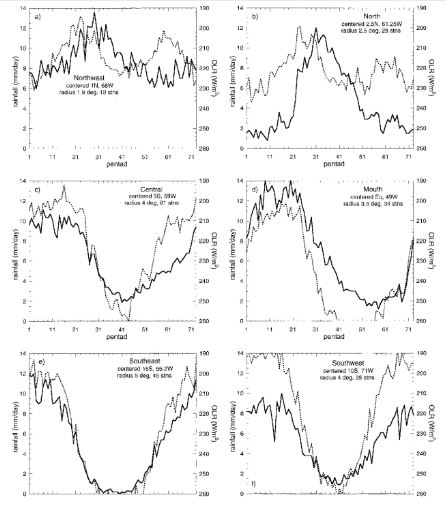
\includegraphics[width=0.7\textwidth,height=\textheight]{imagens/cap04/bo_regioes_climaticas.JPG}

}

\caption{\label{fig-regioes\_climaticas}Regiões climáticas e regimes de
chuva na Amazônia ({[}15{]}).}

\end{figure}%

\begin{figure}[H]

\centering{

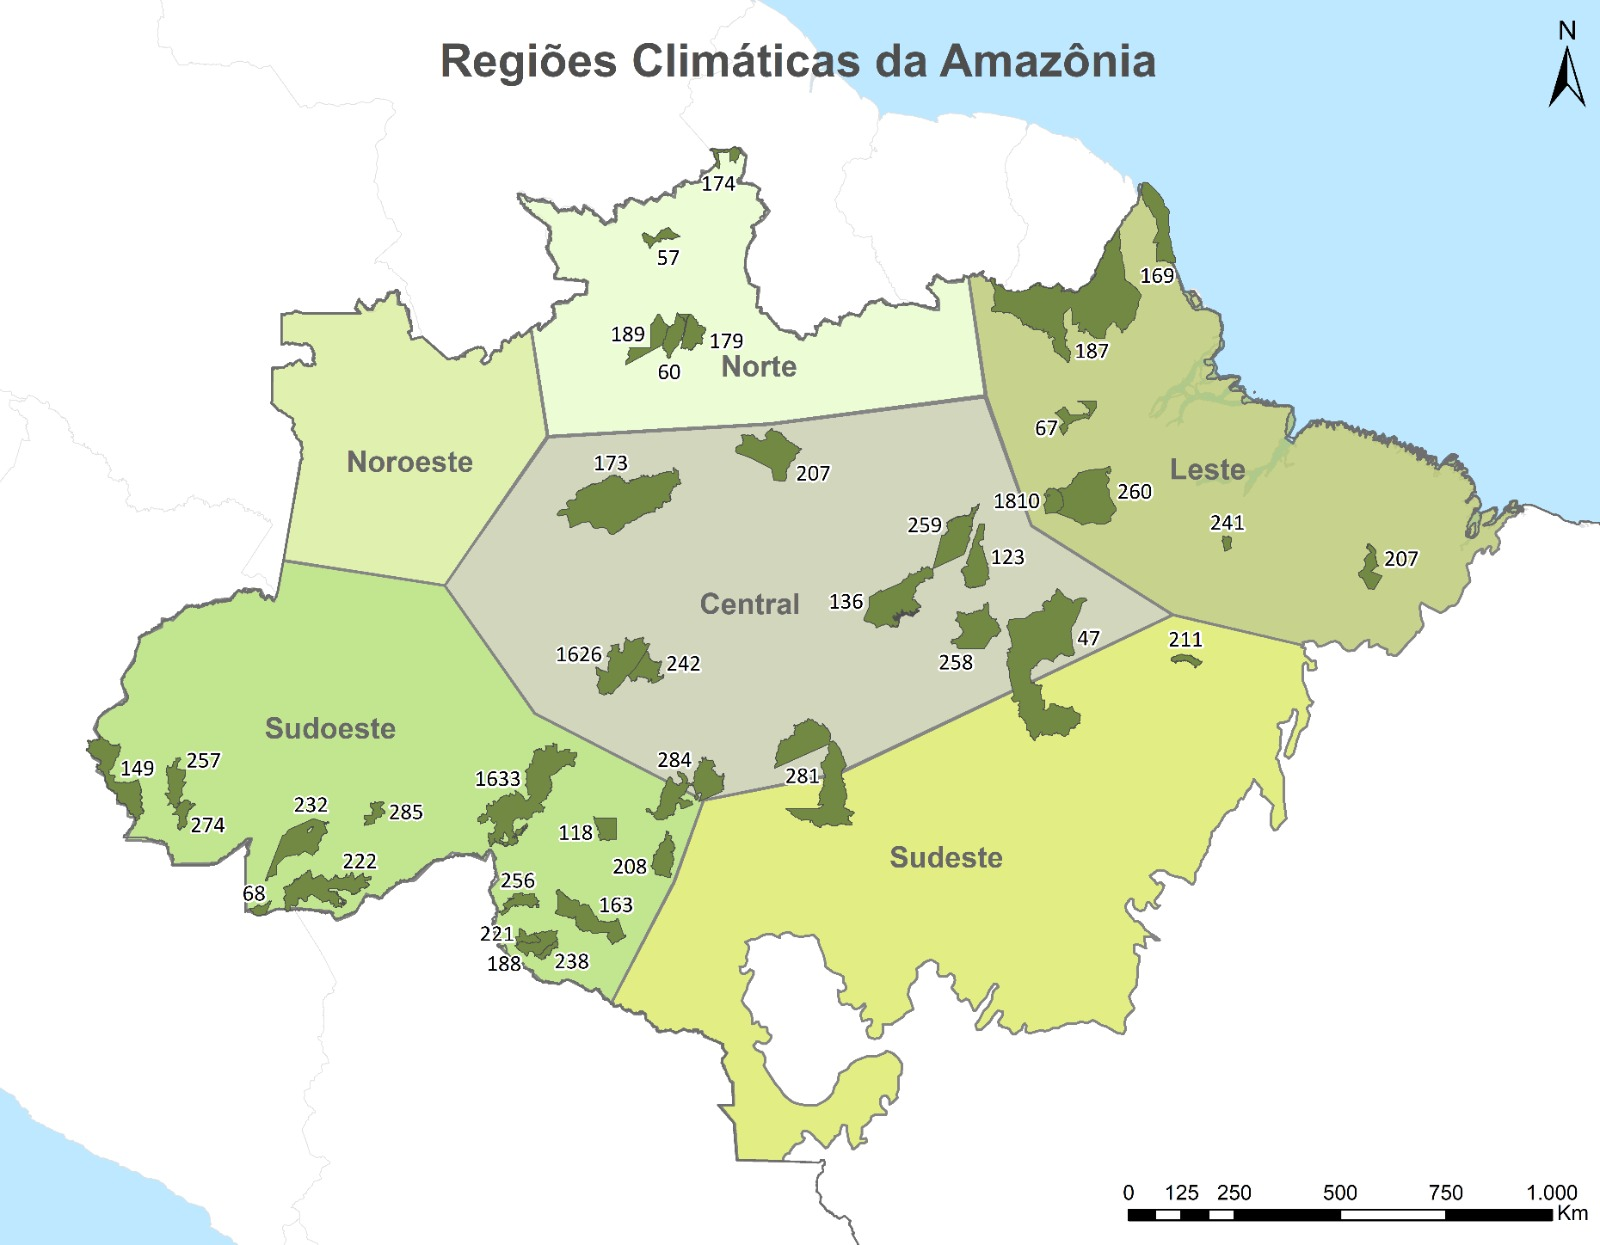
\includegraphics[width=0.7\textwidth,height=\textheight]{imagens/cap04/bo_mapa_ucs.jpeg}

}

\caption{\label{fig-regioes-climaticas}Mapa mostrando a proposta de
distribuição das UCs participantes do Programa Monitora nos polígonos
das regiões climáticas da Amazônia definidos em função do regime de
chuvas.}

\end{figure}%

Tabela x. Localização das UCs em relação às regiões climáticas da
Amazônia, incluindo o período sugerido de amostragens de borboletas
indicado como o final das chuvas. As UCs com * situam-se entre duas ou
mais regiões climáticas (q. = quinzena). As UCs marcadas com \# ainda
não iniciaram a amostragem de borboletas.

\subsubsection{Representação de UCs nas regiões climáticas
amazônicas}\label{representauxe7uxe3o-de-ucs-nas-regiuxf5es-climuxe1ticas-amazuxf4nicas}

Sete UCs da região climática central amazônica realizaram amostragens de
borboletas frugívoras: PARNA do Jaú, REBIO do Uatumã, RESEX
Tapajós-Arapiuns, FLONA do Jamari, REBIO do Jaru, PARNA da Amazônia e
ESEC da Terra do Meio. Essa é a região em que o Programa está mais
consolidado e que possui o maior número de registros e de EAs em
atividade. Devido a isso, será a única região climática analisada
separadamente.

Apesar de termos uma boa representatividade de EAs nos últimos dois anos
e do número considerável de borboletas amostradas, ainda podemos ver
grandes variações entre as proporções de tribos entre os anos
(Figura~\ref{fig-regiao-climatica-central-amazonica}). Considerando as
variações de proporção no número de indivíduos, podemos observar que,
enquanto a tribo Brassolini apresentou tendência de diminuição entre
2014 e 2017, Epicaliini mostrou tendência oposta. Por outro lado, as
tribos Satyrini e Coeini tiveram comportamento errático, variando
amplamente entre anos nesse período. Satyrini é a tribo com maior
contribuição para o total de indivíduos e uma das que sofrem maiores
flutuações. As tribos Callicorini, Biblidini e Ageroniini,
características de ambientes alterados, tiveram baixíssima representação
no conjunto de UCs da região climática central amazônica. Considerando
esse conjunto de variações nas proporções das tribos, a assinatura
regional sofreu consideráveis alterações entre 2014 e 2018
(Figura~\ref{fig-regiao-climatica-central-amazonica}).

Nenhuma UC coletou dados de borboletas frugívoras na região climática
noroeste amazônica, região extremamente chuvosa e que praticamente não
possui um período de estiagem, dificultando a definição do melhor
período de amostragem de borboletas. Mesmo assim, seria importante
tentar implementar a amostragem de borboletas em, pelo menos, três EAs
da RESEX do Baixo Juruá, valendo-se dos parâmetros estabelecidos para a
região climática norte amazônica (Tabela x). A identificação de, pelo
menos, mais duas UCs nessa região para compor o Programa Monitora seria
bastante benéfica para o conjunto de informações geradas em nível
regional amazônico.

As outras quatro regiões climáticas amazônicas possuem dois ou três anos
a menos de dados do que a região Central. Desta forma, as análises para
essas regiões ainda são pouco substanciais e não apresentam tendências
significativas a serem analisadas nesse curto espaço de tempo.

Três UCs estão coletando dados de borboletas frugívoras na região
climática norte amazônica: ESEC Niquiá, ESEC de Maracá e PARNA Serra da
Mocidade. A região iniciou as amostragens em 2017, portanto, é a que
possui menos tempo para definição das frequências normais
(Figura~\ref{fig-regiao-climatica-norte-amazonica}, A).

Quatro UCs da região climática leste amazônica estão coletando dados
para borboletas frugívoras: PARNA do Cabo Orange, PARNA Montanhas do
Tumucumaque, REBIO do Gurupi e RESEX Renascer. A região foi a que
apresentou menores variações entre as proporções de tribos de 2016 a
2018. Essa é uma característica desejável para dados de monitoramento,
pois menores variâncias aumentam o poder de discriminação entre amostras
(Figura~\ref{fig-regiao-climatica-leste-amazonica}).

Sete UCs estão coletando dados para borboletas frugívoras na região
climática sudoeste amazônico: PARNA da Serra do Divisor, PARNA
Mapinguari, PARNA Serra da Cutia, RESEX do Alto Tarauacá, RESEX Barreiro
das Antas, RESEX do Cazumbá-Iracema e RESEX do Rio Ouro Preto. A região
possui um padrão de assinatura de tribos diferente das demais, com
maiores proporções das tribos associadas a ambientes perturbados,
especialmente Ageroniini. A grande variação na proporção de Satyrini e,
em menor grau, Morphini e Brassolini, gerou assinaturas bastante
diferentes entre anos consecutivos na região. Isso também pode ser um
artefato estatístico relacionado ao aumento do número de estações
amostrais e de borboletas amostradas no período, uma vez que estas
variáveis aumentaram mais de seis vezes nesse período
(Figura~\ref{fig-regiao-climatica-sudoeste-amazonica}, C).

Apenas duas UCs da região climática sudeste amazônica estão coletando
dados para borboletas frugívoras: PARNA do Juruena e REBIO do Tapirapé.
Apesar da baixa representação, houve grande homogeneidade entre as áreas
amostradas, o que gerou assinaturas bastante similares entre anos.
Considerando que a metade sul da ESEC da Terra do Meio encontra-se na
região, novas EAs que vierem a ser implementadas nessa porção da UC
poderiam ser adicionadas a esse conjunto regional
(Figura~\ref{fig-regiao-climatica-sudeste-amazonica}, D).

\begin{figure}[H]

\centering{

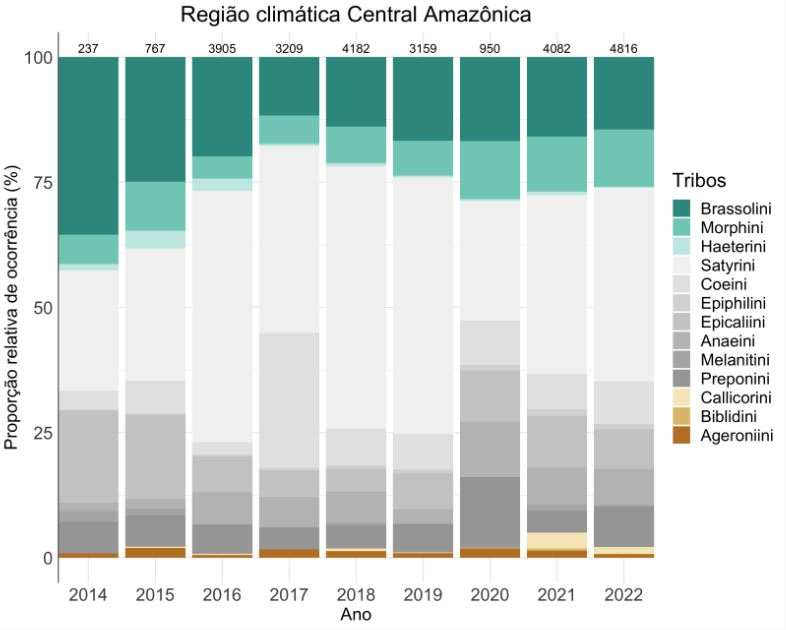
\includegraphics[width=0.7\textwidth,height=\textheight]{imagens/cap04/bo_regiao_climatica_central_amazonica.JPG}

}

\caption{\label{fig-regiao-climatica-central-amazonica}Padrões de bandas
de abundância relativa de tribos de borboletas frugívoras para o período
de 2014 a 2018 na região climática central da Amazônia. Números de
indivíduos amostrados são indicados sobre as barras verticais.}

\end{figure}%

\begin{figure}[H]

\centering{

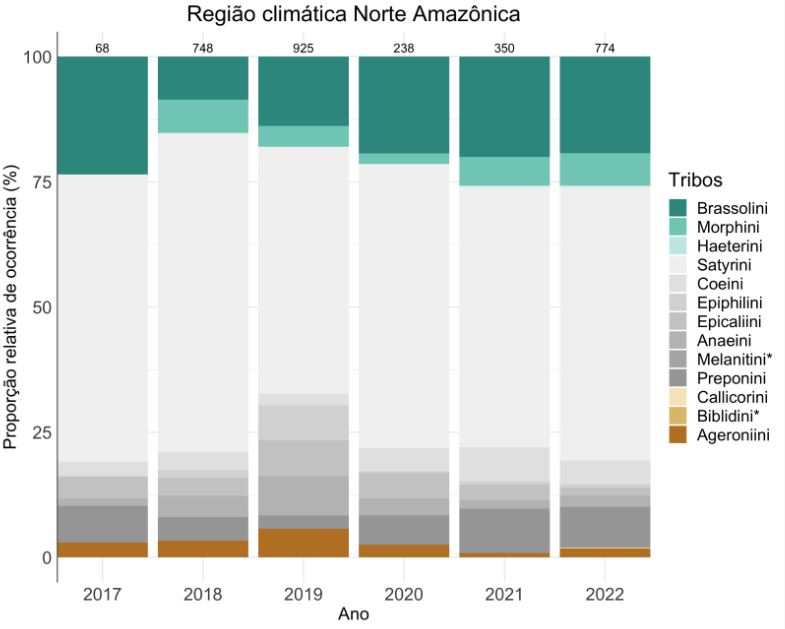
\includegraphics[width=0.7\textwidth,height=\textheight]{imagens/cap04/bo_regiao_climatica_norte_amazonica.JPG}

}

\caption{\label{fig-regiao-climatica-norte-amazonica}Padrões de bandas
de abundância relativa de tribos de borboletas frugívoras para o período
de 2014 a 2018 na região climática norte da Amazônia. Números de
indivíduos amostrados são indicados sobre as barras verticais.}

\end{figure}%

\begin{figure}[H]

\centering{

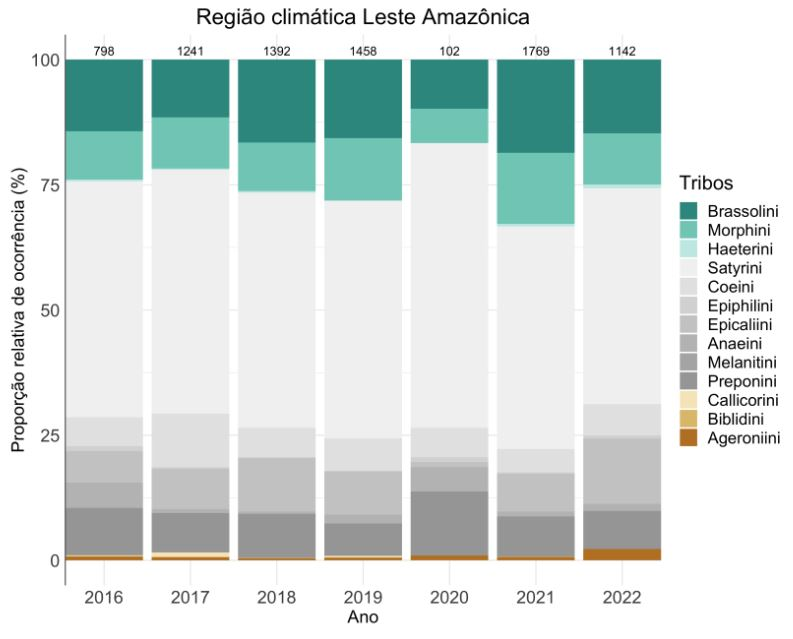
\includegraphics[width=0.7\textwidth,height=\textheight]{imagens/cap04/bo_regiao_climatica_leste_amazonica.JPG}

}

\caption{\label{fig-regiao-climatica-leste-amazonica}Padrões de bandas
de abundância relativa de tribos de borboletas frugívoras para o período
de 2014 a 2018 na região climática leste da Amazônia. Números de
indivíduos amostrados são indicados sobre as barras verticais.}

\end{figure}%

\begin{figure}[H]

\centering{

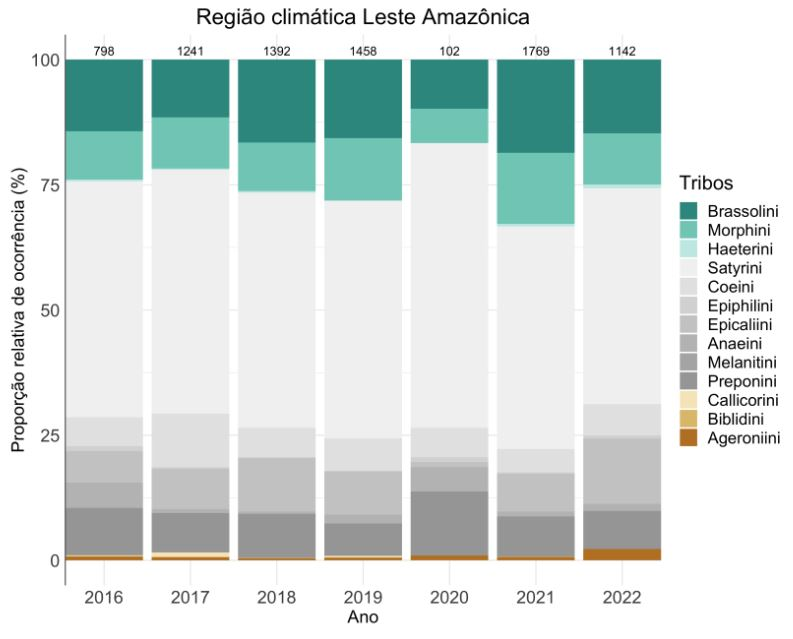
\includegraphics[width=0.7\textwidth,height=\textheight]{imagens/cap04/bo_regiao_climatica_leste_amazonica.JPG}

}

\caption{\label{fig-regiao-climatica-sudoeste-amazonica}Padrões de
bandas de abundância relativa de tribos de borboletas frugívoras para o
período de 2014 a 2018 na região climática sudoeste da Amazônia. Números
de indivíduos amostrados são indicados sobre as barras verticais.}

\end{figure}%

\begin{figure}[H]

\centering{

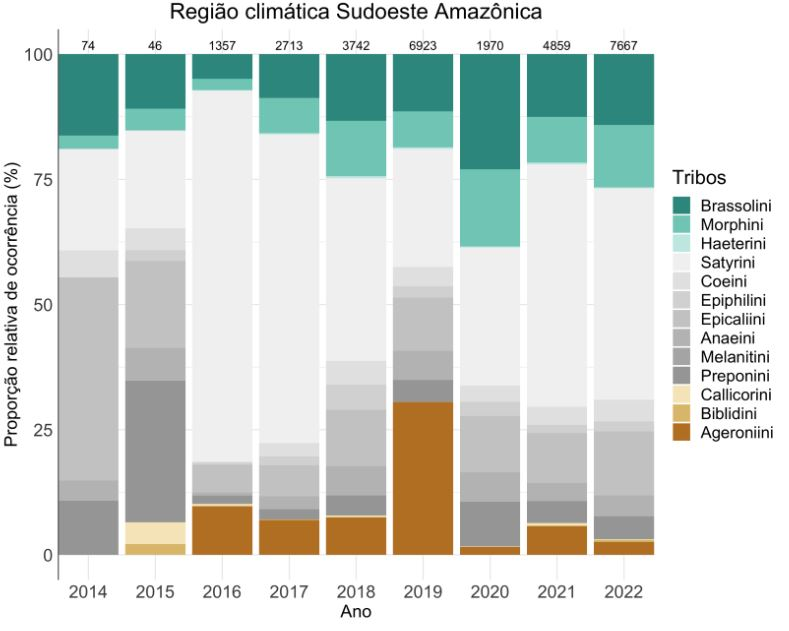
\includegraphics[width=0.7\textwidth,height=\textheight]{imagens/cap04/bo_regiao_climatica_sudoeste_amazonica.JPG}

}

\caption{\label{fig-regiao-climatica-sudeste-amazonica}Padrões de bandas
de abundância relativa de tribos de borboletas frugívoras para o período
de 2014 a 2018 na região climática sudeste da Amazônia. Números de
indivíduos amostrados são indicados sobre as barras verticais.}

\end{figure}%

\subsection{Cerrado e Mata Atlântica}\label{cerrado-e-mata-atluxe2ntica}

\begin{figure}[H]

\centering{

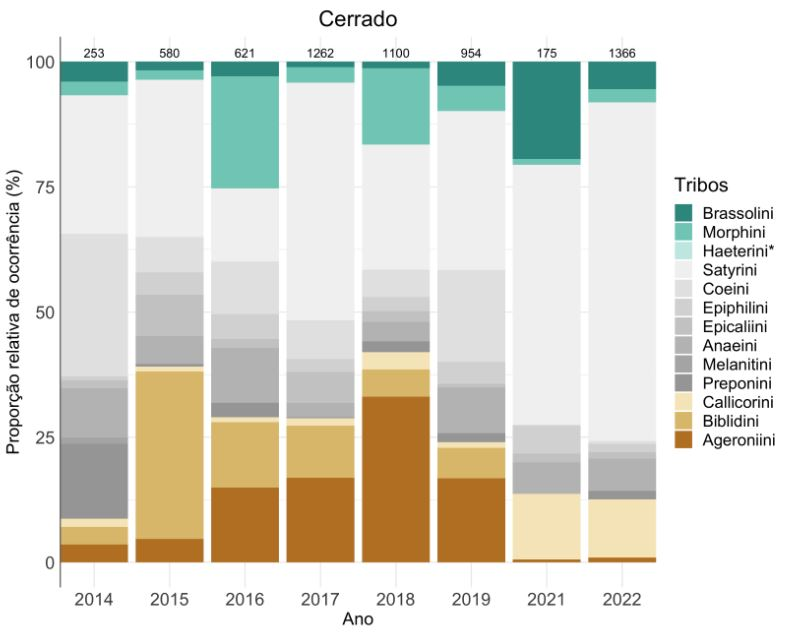
\includegraphics[width=0.7\textwidth,height=\textheight]{imagens/cap04/bo_cerrado.JPG}

}

\caption{\label{fig-regiao-cerrado}Padrões de bandas de abundância
relativa de tribos de borboletas frugívoras para o período de 2014 a
2018 no bioma Cerrado. Números de indivíduos amostrados são indicados
sobre as barras verticais.}

\end{figure}%

\begin{figure}[H]

\centering{

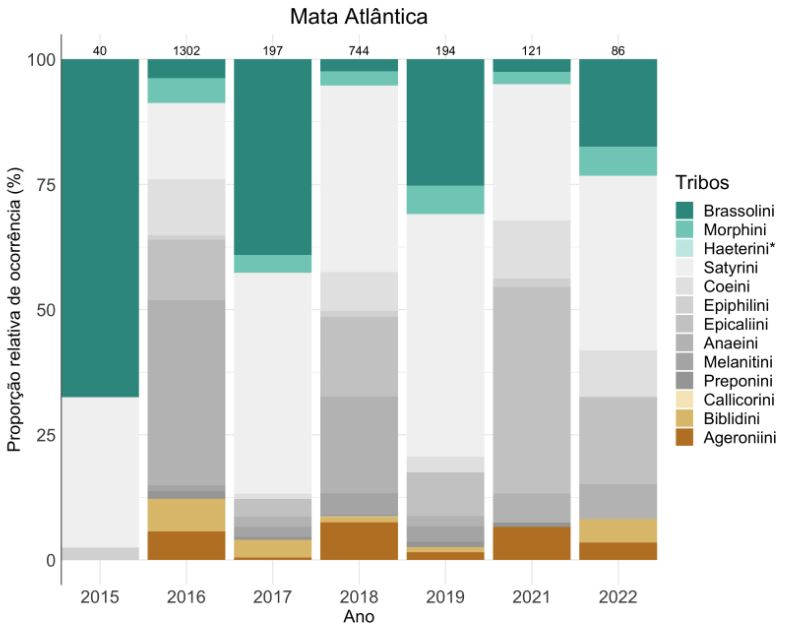
\includegraphics[width=0.7\textwidth,height=\textheight]{imagens/cap04/bo_mata_atlantica.JPG}

}

\caption{\label{fig-regiao-mata\_atlantica}Padrões de bandas de
abundância relativa de tribos de borboletas frugívoras para o período de
2014 a 2018 no bioma Mata Atlântica. Números de indivíduos amostrados
são indicados sobre as barras verticais.}

\end{figure}%

\subsection{Índice de abundância de
tribos}\label{uxedndice-de-abunduxe2ncia-de-tribos}

A análise a seguir ainda está em fase de teste conceitual, tanto no
modelo estatístico quanto no significado biológico. Esse tipo de cálculo
geralmente é feito com dados populacionais (abundância de indivíduos),
tendo seu cálculo e seu significado biológico já consagrados em diversos
países (e.g., {[}16{]}). Assim, essa proposta visa criar um índice
aplicável em nível de tribo e gerar análises para testar a sua
viabilidade para o Programa Monitora. Caso adotado, esse índice pode
servir de base para o monitoramento de flutuações de abundância
diferentemente da abordagem das assinaturas, que é feita de forma
qualitativa. Entendemos que o Programa Monitora necessita de abordagens
mais quantitativas que possibilitem a definição de níveis de variação
sobre os quais possam ser gerados alertas para atenção ou verificação
pela gestão da UC.

\subsubsection{Cálculo do índice}\label{cuxe1lculo-do-uxedndice}

O índice tem como base o número acumulado de indivíduos de cada tribo
para cada ano de uma dada área. Partindo da frequência absoluta de
indivíduos por tribo por ano (n), fazemos inicialmente uma correção,
somando um número muito pequeno a cada frequência absoluta, de forma a
evitar a presença de zeros na matriz. Desta forma é obtida a frequência
absoluta corrigida (f = n + 0,00001). Em seguida, é calculada a
frequência corrigida pelo esforço amostral (número de armadilhas * dias
de amostragem) (fe). Considerando que essa frequência mostra grandes
variações, às vezes em duas ordens de grandeza, optamos por realizar uma
transformação logarítmica para normalizar os dados. Assim, o próximo
passo é calcular o log10 da fe. O índice é finalmente calculado,
comparando-se as variações da fe em anos consecutivos, considerando-se
sempre o índice igual a 1,0 para o primeiro ano em que aquela
``população'' foi registrada. A Tabela x mostra o produto desse cálculo.
Note-se que o ano base para algumas tribos difere do ano base da maioria
das outras.

Tabela x. Matriz resultante do cálculo das frequências absolutas
divididas pelo esforço amostral, normalizadas (Log10) e transformadas em
índice ``populacional'' para rastrear as variações a partir do ano em
que uma ``população'' foi detectada (i = 1,000); i = índice de
abundância a partir do ano base.

\subsection{Análises regionais}\label{anuxe1lises-regionais}

Assim como foi feito na seção anterior, utilizaremos os mesmos conjuntos
de dados regionais para explorar a viabilidade de uso do índice
proposto. A região climática central foi analisada separadamente por ser
a única que possui dados para cinco anos consecutivos. Apesar de tanto a
composição de UCs quanto o esforço amostral terem se multiplicado cinco
vezes nesse período (Tabela x), ainda assim este é o melhor conjunto de
dados que possuímos para gerar tais análises.

Considerando que a visualização das 13 tribos em um mesmo gráfico impede
a identificação do comportamento das curvas individualmente, optamos por
apresentar dois gráficos para cada região com as tribos mais
representativas de ambientes bem preservados e de ambientes mais
perturbados. Assim, as variações dos índices para cada uma dessas tribos
para a região climática central amazônica podem ser observadas a seguir
(Figura~\ref{fig-IA-regiao-climatica-central-amazonica},
Figura~\ref{fig-IA-areas-abertas-regiao-climatica-central-amazonica}). O
ano base é considerado como o início da ``população'' monitorada e tem
sempre o valor igual a 1,0. As mudanças subsequentes mostram variações
baseadas nessa população inicial, sendo que variações acima da linha de
base indicam crescimento populacional e, abaixo desta, diminuição. Quase
todas as tribos apresentaram o mesmo padrão de variação nesse período.
Houve uma pequena diminuição em 2015 e 2016, seguido de um grande
aumento em 2017 e um decréscimo posterior em 2018. É interessante
observar que a tribo que apresentou menor variação no período foi
Ageroniini, seguida de Morphini.

Já para as demais regiões climáticas amazônicas, o esforço amostral e a
quantidade de dados obtidos até 2018 foi inferior ao obtido para a
região central e ainda foi insuficiente para observar alterações
significativas. A região norte passou a gerar dados apenas a partir de
2017 e ainda possui poucas EAs para compor essa análise. As regiões
leste e sudoeste já possuem um bom número de EAs e, em poucos anos,
terão dados suficientes para análise. A região sudeste ainda está em
processo de implementação e necessita de mais adesões para gerar um
conjunto de dados adequado para análise. Essa região vem contabilizando
os melhores retornos de captura por unidade de esforço (CPUE), tendo
amostrado bem mais borboletas do que as outras regiões para uma dada
quantidade de esforço (Tabela x), exceto a região central (Tabela x).

A abundância das tribos variou sem uma tendência predominante durante o
período de 2016 a 2018 nas regiões climáticas norte, leste, sudoeste e
sudeste amazônicas. Algumas tribos apresentaram picos de abundância para
cima ou para baixo durante esses primeiros anos, como Callicorini, na
região sudoeste, em 2017, e Biblidini, nas regiões leste e sudeste, em
2017. Porém, a maioria das tribos encontravam-se, em 2018, próximas do
valor original (1,0) (Figura x). Essas tribos apresentaram tamanhos
populacionais muito pequenos em quase todas as UCs durante esse período.

Consequentemente, qualquer variação na quantidade de borboletas
capturadas causou grandes variações no índice de abundância. Portanto,
concluímos que o uso desse índice para ``populações'' pequenas não é
aconselhável. Neste caso, o tamanho amostral pode ser a solução para o
problema, pois traria uma quantidade maior de dados e, supostamente,
menores variações.

Tabela x. Soma do número de indivíduos e esforço amostral (nº de EAs x
nº de armadilhas x 12 dias de amostragem) no conjunto de sete UCs da
região climática central amazônica. Esforço amostral em armadilhas x
dia.

\begin{figure}[H]

\centering{

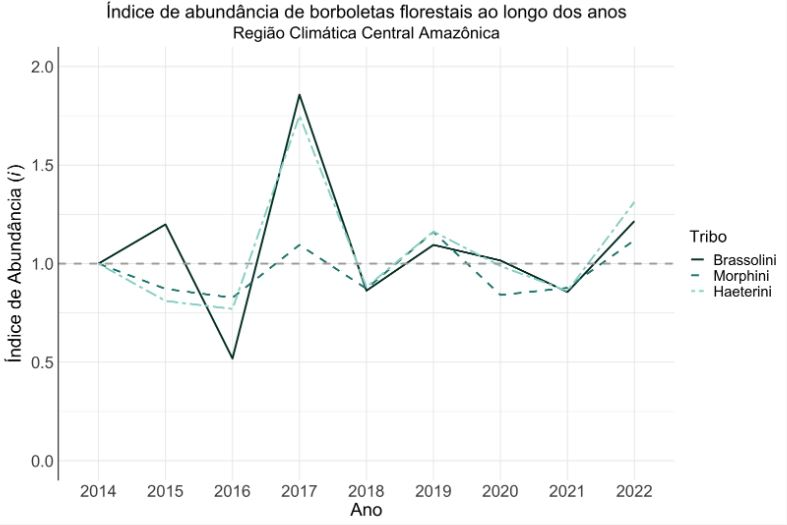
\includegraphics[width=0.7\textwidth,height=\textheight]{imagens/cap04/bo_IA_regiao_climatica_central_amazonica.JPG}

}

\caption{\label{fig-IA-regiao-climatica-central-amazonica}Variação no
índice de abundância das tribos de borboletas frugívoras indicadoras de
florestas íntegras (tons de verde) e de florestas perturbadas (tons de
laranja) na região climática central da Amazônia, no período de 2014 a
2022.}

\end{figure}%

\begin{figure}[H]

\centering{

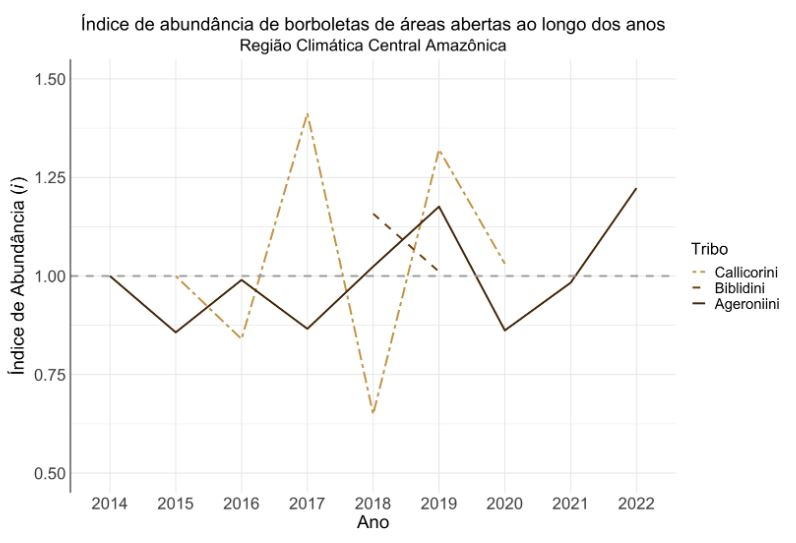
\includegraphics[width=0.7\textwidth,height=\textheight]{imagens/cap04/bo_IA_areas_abertas_regiao_climatica_central_amazonica.JPG}

}

\caption{\label{fig-IA-areas-abertas-regiao-climatica-central-amazonica}Variação
no índice de abundância das tribos de borboletas frugívoras indicadoras
de florestas íntegras (tons de verde) e de florestas perturbadas (tons
de laranja) na região climática central da Amazônia, no período de 2014
a 2022.}

\end{figure}%

\begin{figure}[H]

\centering{

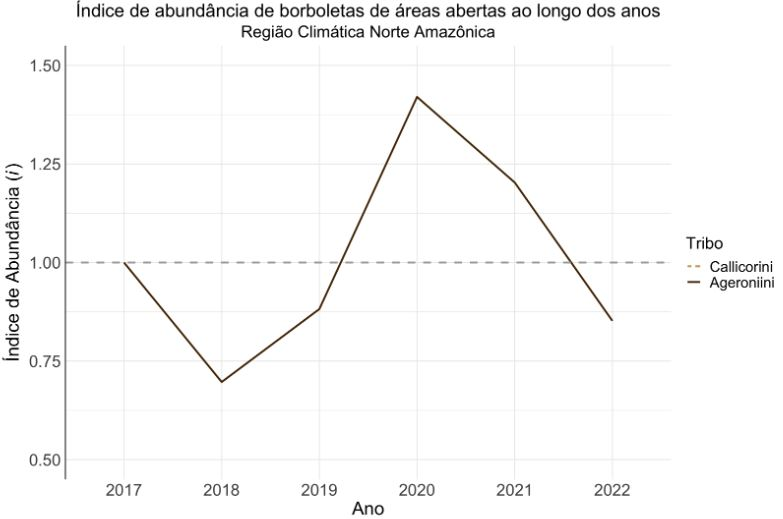
\includegraphics[width=0.7\textwidth,height=\textheight]{imagens/cap04/bo_IA_areas_abertas_regiao_climatica_norte_amazonica.JPG}

}

\caption{\label{fig-IA-regiao-climatica-norte-amazonica}Variação no
índice de abundância das tribos de borboletas frugívoras indicadoras de
florestas íntegras (tons de verde) e de florestas perturbadas (tons de
laranja) na região climática norte da Amazônia, no período de 2014 a
2022.}

\end{figure}%

\begin{figure}[H]

\centering{

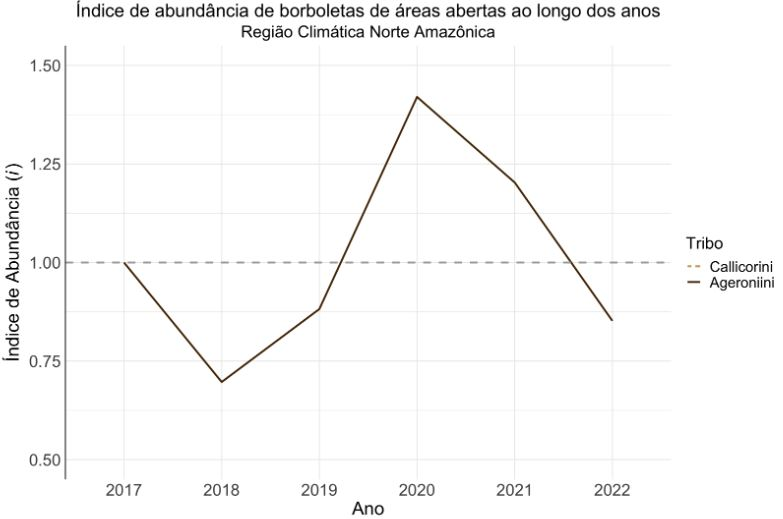
\includegraphics[width=0.7\textwidth,height=\textheight]{imagens/cap04/bo_IA_areas_abertas_regiao_climatica_norte_amazonica.JPG}

}

\caption{\label{fig-IA-areas-abertas-regiao-climatica-norte-amazonica}Variação
no índice de abundância das tribos de borboletas frugívoras indicadoras
de florestas íntegras (tons de verde) e de florestas perturbadas (tons
de laranja) na região climática norte da Amazônia, no período de 2014 a
2022.}

\end{figure}%

\begin{figure}[H]

\centering{

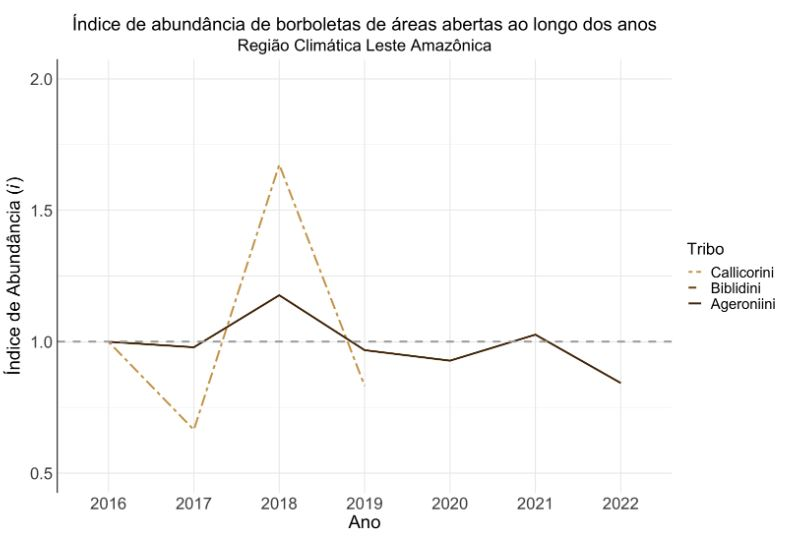
\includegraphics[width=0.7\textwidth,height=\textheight]{imagens/cap04/bo_IA_areas_abertas_regiao_climatica_leste_amazonica.JPG}

}

\caption{\label{fig-IA-regiao-climatica-leste-amazonica}Variação no
índice de abundância das tribos de borboletas frugívoras indicadoras de
florestas íntegras (tons de verde) e de florestas perturbadas (tons de
laranja) na região climática leste da Amazônia, no período de 2014 a
2022.}

\end{figure}%

\begin{figure}[H]

\centering{

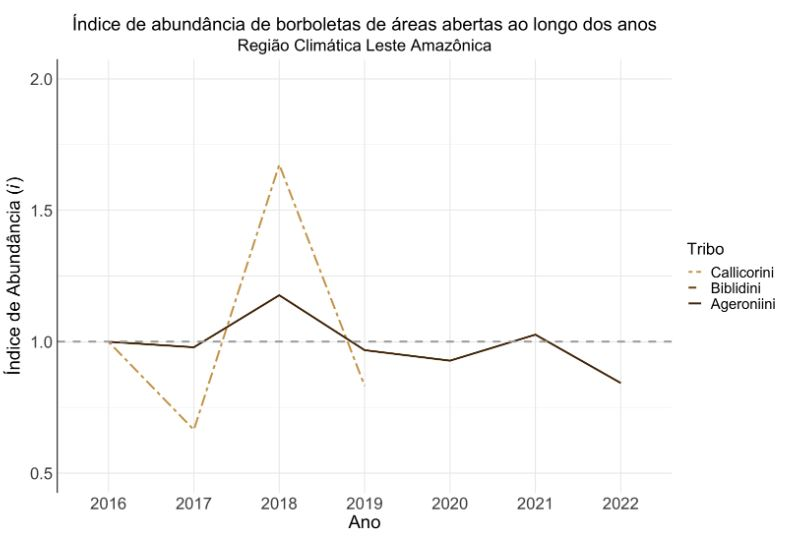
\includegraphics[width=0.7\textwidth,height=\textheight]{imagens/cap04/bo_IA_areas_abertas_regiao_climatica_leste_amazonica.JPG}

}

\caption{\label{fig-IA-areas-abertas-regiao-climatica-leste-amazonica}Variação
no índice de abundância das tribos de borboletas frugívoras indicadoras
de florestas íntegras (tons de verde) e de florestas perturbadas (tons
de laranja) na região climática leste da Amazônia, no período de 2014 a
2022.}

\end{figure}%

\begin{figure}[H]

\centering{

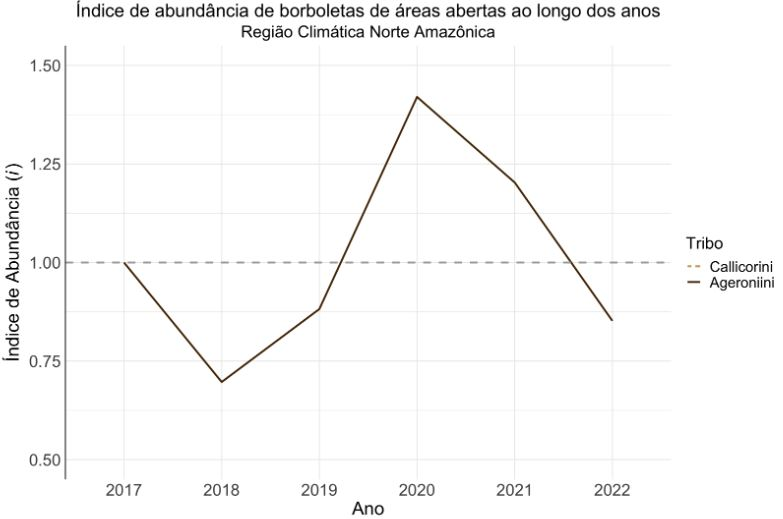
\includegraphics[width=0.7\textwidth,height=\textheight]{imagens/cap04/bo_IA_areas_abertas_regiao_climatica_norte_amazonica.JPG}

}

\caption{\label{fig-IA-regiao-climatica-sudoeste-amazonica}Variação no
índice de abundância das tribos de borboletas frugívoras indicadoras de
florestas íntegras (tons de verde) e de florestas perturbadas (tons de
laranja) na região climática norte da Amazônia, no período de 2014 a
2022.}

\end{figure}%

\begin{figure}[H]

\centering{

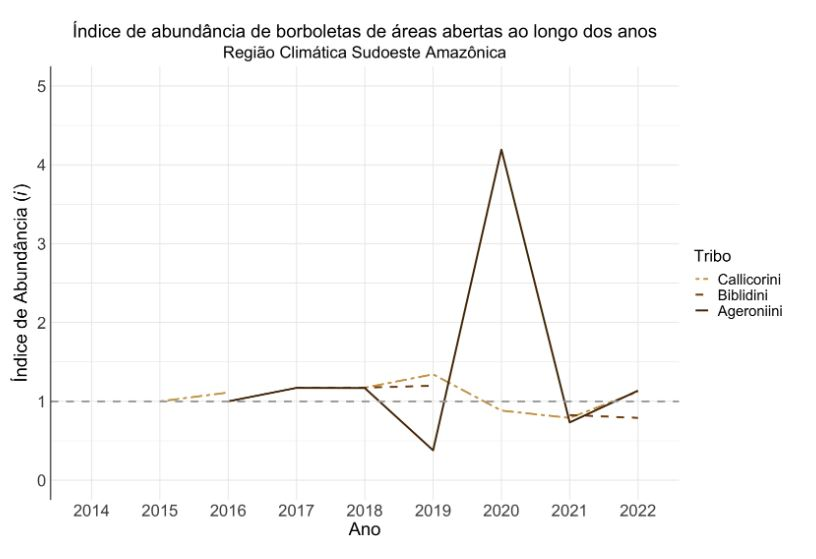
\includegraphics[width=0.7\textwidth,height=\textheight]{imagens/cap04/bo_IA_areas_abertas_regiao_climatica_sudoeste_amazonica.JPG}

}

\caption{\label{fig-IA-areas-abertas-regiao-climatica-sudoeste-amazonica}Variação
no índice de abundância das tribos de borboletas frugívoras indicadoras
de florestas íntegras (tons de verde) e de florestas perturbadas (tons
de laranja) na região climática sudoeste da Amazônia, no período de 2014
a 2022.}

\end{figure}%

\begin{figure}[H]

\centering{

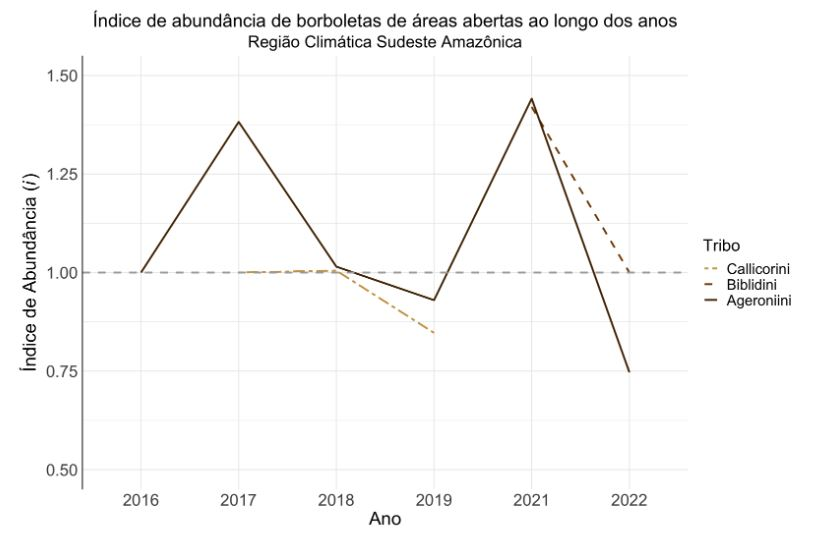
\includegraphics[width=0.7\textwidth,height=\textheight]{imagens/cap04/bo_IA_areas_abertas_regiao_climatica_sudeste_amazonica.JPG}

}

\caption{\label{fig-IA-regiao-climatica-sudeste-amazonica}Variação no
índice de abundância das tribos de borboletas frugívoras indicadoras de
florestas íntegras (tons de verde) e de florestas perturbadas (tons de
laranja) na região climática sudeste da Amazônia, no período de 2014 a
2022.}

\end{figure}%

\begin{figure}[H]

\centering{

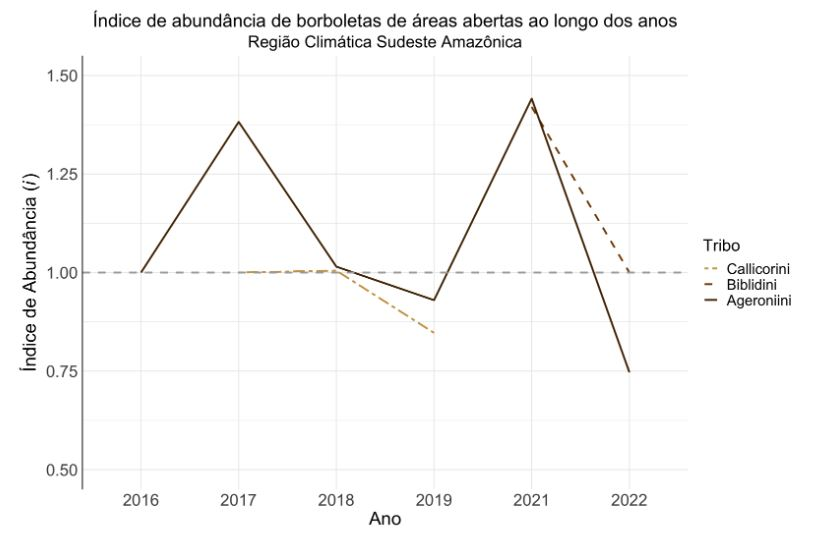
\includegraphics[width=0.7\textwidth,height=\textheight]{imagens/cap04/bo_IA_areas_abertas_regiao_climatica_sudeste_amazonica.JPG}

}

\caption{\label{fig-IA-areas-abertas-regiao-climatica-sudeste-amazonica}Variação
no índice de abundância das tribos de borboletas frugívoras indicadoras
de florestas íntegras (tons de verde) e de florestas perturbadas (tons
de laranja) na região climática sudeste da Amazônia, no período de 2014
a 2022.}

\end{figure}%

\begin{figure}[H]

\centering{

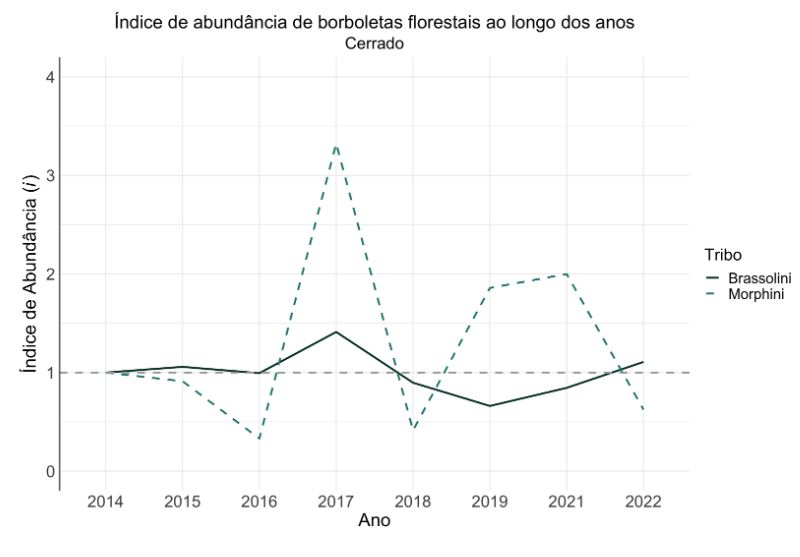
\includegraphics[width=0.7\textwidth,height=\textheight]{imagens/cap04/bo_IA_cerrado.JPG}

}

\caption{\label{fig-IA-cerrado}Variação no índice de abundância das
tribos de borboletas frugívoras indicadoras de florestas íntegras (tons
de verde) e de florestas perturbadas (tons de laranja) no bioma Cerrado,
no período de 2014 a 2022.}

\end{figure}%

\begin{figure}[H]

\centering{

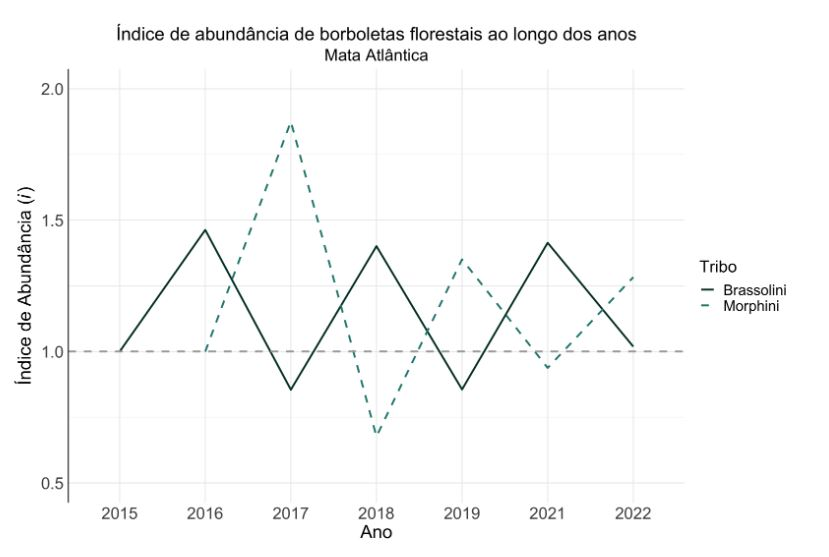
\includegraphics[width=0.7\textwidth,height=\textheight]{imagens/cap04/bo_IA_mata_atlantica.JPG}

}

\caption{\label{fig-IA-mata-atlantica}Variação no índice de abundância
das tribos de borboletas frugívoras indicadoras de florestas íntegras
(tons de verde) e de florestas perturbadas (tons de laranja) no bioma
Mata Atlântica, no período de 2014 a 2022.}

\end{figure}%

\subsection{Destaques}\label{destaques-1}

\subsubsection{Efeito da seca extrema de 2015 nas UCs da região Central
Amazônica**}\label{efeito-da-seca-extrema-de-2015-nas-ucs-da-regiuxe3o-central-amazuxf4nica}

\subsubsection{Efeito da queda dos tabocais na RESEX Cazumbá-Iracema e
Riozinho da Liberdade e Serra do Divisor
(controle)**}\label{efeito-da-queda-dos-tabocais-na-resex-cazumbuxe1-iracema-e-riozinho-da-liberdade-e-serra-do-divisor-controle}

\begin{figure}[H]

\centering{

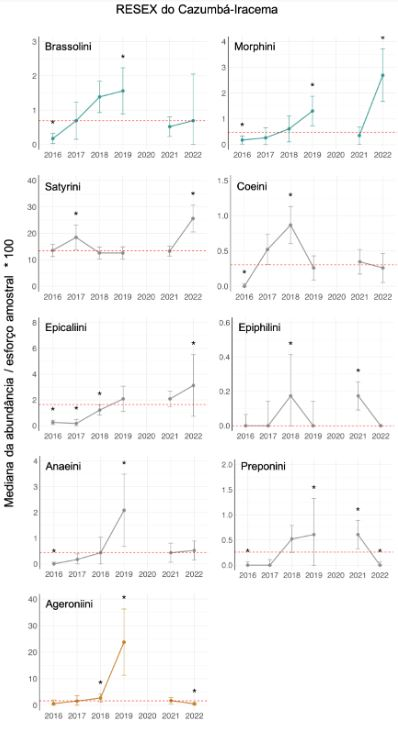
\includegraphics[width=0.7\textwidth,height=\textheight]{imagens/cap04/bo_abundancia_resex_cazumba_iracema.JPG}

}

\caption{\label{fig-abundancia-resex-cazumba-iracema}Variação na
abundância das tribos de borboletas frugívoras na RESEX do
Cazumbá-Iracema no período de 2016 a 2022.}

\end{figure}%

\begin{figure}[H]

\centering{

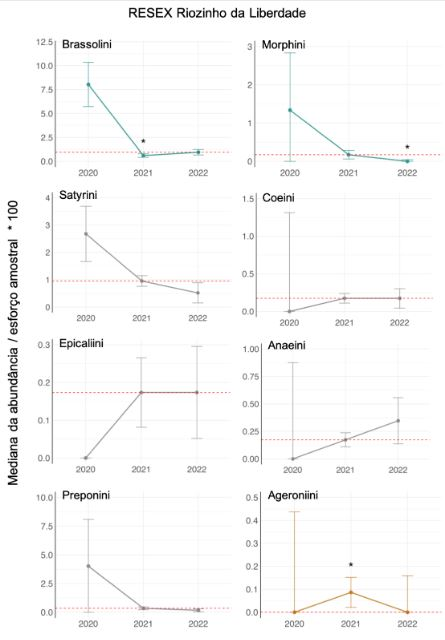
\includegraphics[width=0.7\textwidth,height=\textheight]{imagens/cap04/bo_abundancia_resex_riozinho_liberdade.jpg}

}

\caption{\label{fig-abundancia-resex-riozinho-liberdade}Variação na
abundância das tribos de borboletas frugívoras na RESEX do Riozinho da
Liberdade no período de 2020 a 2022.}

\end{figure}%

\begin{figure}[H]

\centering{

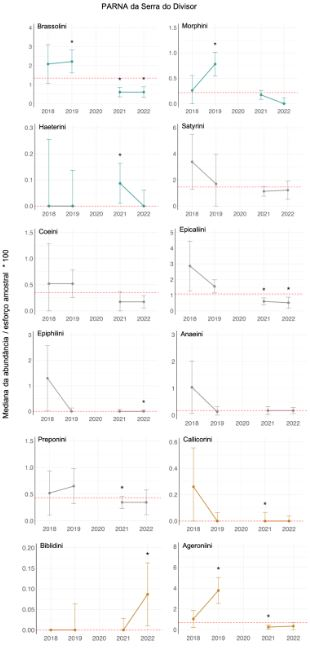
\includegraphics[width=0.7\textwidth,height=\textheight]{imagens/cap04/bo_abundancia_parna_serra_divisor.jpg}

}

\caption{\label{fig-abundancia-parna-serra-divisor}Variação na
abundância das tribos de borboletas frugívoras no PARNA da Serra do
Divisor no período de 2018 a 2022.}

\end{figure}%

\section{Discussão}\label{discussuxe3o-1}

\emph{There are many variations of passages of Lorem Ipsum available,
but the majority have suffered alteration in some form, by injected
humour, or randomised words which don't look even slightly believable.
If you are going to use a passage of Lorem Ipsum, you need to be sure
there isn't anything embarrassing hidden in the middle of text. All the
Lorem Ipsum generators on the Internet tend to repeat predefined chunks
as necessary, making this the first true generator on the Internet. It
uses a dictionary of over 200 Latin words, combined with a handful of
model sentence structures, to generate Lorem Ipsum which looks
reasonable. The generated Lorem Ipsum is therefore always free from
repetition, injected humour, or non-characteristic words etc.}

\section{Recomendações}\label{recomendauxe7uxf5es-1}

\emph{There are many variations of passages of Lorem Ipsum available,
but the majority have suffered alteration in some form, by injected
humour, or randomised words which don't look even slightly believable.
If you are going to use a passage of Lorem Ipsum, you need to be sure
there isn't anything embarrassing hidden in the middle of text. All the
Lorem Ipsum generators on the Internet tend to repeat predefined chunks
as necessary, making this the first true generator on the Internet. It
uses a dictionary of over 200 Latin words, combined with a handful of
model sentence structures, to generate Lorem Ipsum which looks
reasonable. The generated Lorem Ipsum is therefore always free from
repetition, injected humour, or non-characteristic words etc.}

\bookmarksetup{startatroot}

\chapter{Mamíferos e aves}\label{mamuxedferos-e-aves}

\textbf{Arlindo Gomes Filho\textsuperscript{1}, Elildo Alves Ribeiro de
Carvalho Junior\textsuperscript{2}, Gerson Buss\textsuperscript{3},
Marcelo Lima Reis\textsuperscript{4}, Marcos de Sousa
Fialho\textsuperscript{1}, Rafael Suertegaray
Rossato\textsuperscript{3}, Ricardo Sampaio\textsuperscript{3}, Richard
Hatakeyama\textsuperscript{5}, Thiago Orsi
Laranjeiras\textsuperscript{6}}

\begin{enumerate}
\def\labelenumi{\arabic{enumi}.}
\item
  Centro Nacional de Pesquisa e Conservação de Aves Silvestres --
  CEMAVE\\
  \emph{Instituto Chico Mendes de Conservação da Biodiversidade --
  ICMBio}\\
  \emph{BR-230 Km 10}\\
  \emph{Floresta Nacional da Restinga de Cabedelo}\\
  \emph{58108-012 Cabedelo, PB}
\item
  Centro Nacional de Pesquisa e Conservação de Mamíferos Carnívoros --
  CENAP\\
  \emph{Instituto Chico Mendes de Conservação da Biodiversidade --
  ICMBio}\\
  \emph{Estrada Municipal Hisaichi Takebayashi, 8600 - Bairro da Usina}
  \emph{12952-011 Atibaia, SP}
\item
  Centro Nacional de Pesquisa e Conservação de Primatas Brasileiros --
  CPB\\
  \emph{Instituto Chico Mendes de Conservação da Biodiversidade --
  ICMBio}\\
  \emph{BR-230 Km 10}\\
  \emph{Floresta Nacional da Restinga de Cabedelo}\\
  \emph{58108-012 Cabedelo, PB}
\item
  Coordenação de Monitoramento da Biodiversidade - COMOB\\
  \emph{Instituto Chico Mendes de Conservação da Biodiversidade --
  ICMBio}\\
  \emph{Complexo Administrativo EQSW 103/104 s/n}\\
  \emph{70670-350 Brasília, DF}
\item
  Núcleo de Gestão Integrada - NGI ICMBio Tefé\\
  \emph{Instituto Chico Mendes de Conservação da Biodiversidade --
  ICMBio}\\
  \emph{Estr. do Aeroporto, 725 - Centro}\\
  \emph{69550-101 Tefé, AM}
\item
  Parque Nacional do Viruá\\
  \emph{Instituto Chico Mendes de Conservação da Biodiversidade --
  ICMBio}\\
  \emph{69360-000 Caracaraí, RR}
\end{enumerate}

Mamíferos e aves florestais de médio e grande porte são animais que
sofrem muita pressão com a caça e, portanto, são considerados
indicadores de impactos de origem antrópica. A defaunação das florestas
acarreta a chamada ``síndrome da floresta vazia'' ({[}17{]}). A redução
das populações animais além de ser uma diminuição direta da
biodiversidade, também acomete a própria estrutura e manutenção das
florestas, ao perder polinizadores, dispersores de sementes e outros
processos ecológicos importantes. Daí a necessidade de realizar o
monitoramento desses dois grupos no âmbito do Programa Monitora.

A taxonomia utilizada para os mamíferos e aves foi a mesma adotada no
processo de avaliação do estado de conservação das espécies da fauna
brasileira ({[}18{]}).

\section{Estado da implementação}\label{estado-da-implementauxe7uxe3o-2}

Para o período de 2014 a 2022 foram registradas 52 UCs federais e 138
UAs (transecções lineares) em operação, isto é, com amostragens dos
alvos mamíferos e aves com o método do protocolo básico (censo diurno em
transecção linear), nos biomas Amazônia, Cerrado e Mata Atlântica.

Destas 52 UCs federais com coleta de dados de mamíferos e aves, 34
(67\%) já estão consolidadas, isto é, possuem pelo menos três unidades
amostrais (transecções lineares) em operação. Seis UCs retomaram as
amostragens em 2022, sete UCs são consideradas como paradas ou
interrompidas (mais de dois anos consecutivos sem amostragem) e duas UCs
não fizeram amostragens de 2022
(Figura~\ref{fig-esforco-total-uc-bioma}).

O esforço de amostragem nos nove anos considerados neste relatório
correspondeu a 5.356 dias de campo (transecção/dia) e 25.602,55 km
percorridos (Figura~\ref{fig-esforco-acumulado}), resultando em 22.985
registros de mamíferos de médio e grande porte e de 12.995 aves
terrestres cinegéticas (Figura~\ref{fig-taxons-acumulados}). No total,
foram identificados ?? táxons de Mamíferos e 38 de Aves entre gêneros e
espécies (Apêndice C), ?? e 6 dos quais estão ameaçados de extinção,
respectivamente. O esforço por UC, ordenadas por bioma (Mata Atlântica,
Cerrado e Amazônia), é apresentado na
Figura~\ref{fig-esforco-total-uc-bioma}.

\begin{figure}[H]

\centering{

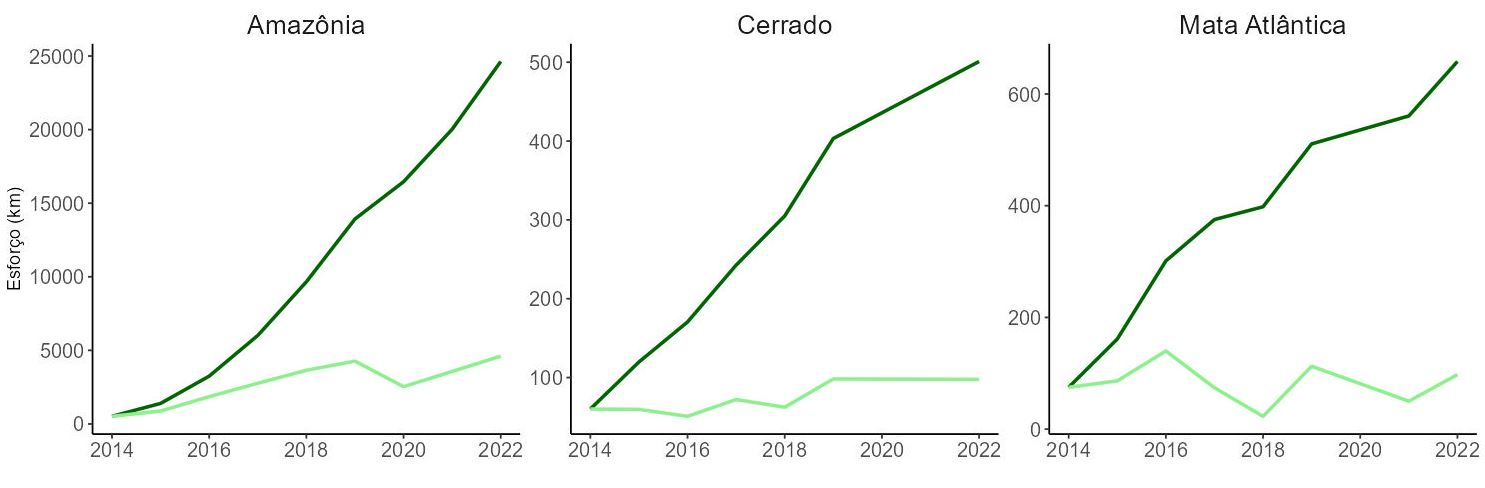
\includegraphics[width=0.8\textwidth,height=\textheight]{imagens/cap05/ma_esforco_acumulado1.JPG}

}

\caption{\label{fig-esforco-acumulado}Esforço por ano e acumulado em
quilômetros percorridos nas unidades de conservação aderidas ao Programa
Monitora entre 2014 e 2022.}

\end{figure}%

\begin{figure}[H]

\centering{


\includegraphics[width=0.7\textwidth,height=\textheight]{imagens/cap05/ma_ucs_ativas_taxa_acumulado1.JPG}

}

\caption{\label{fig-taxons-acumulados}Táxons registrados acumulados e
número de unidades de conservação com protocolo básico de masto-aves
executado por ano entre 2014 e 2022.}

\end{figure}%

\begin{figure}

\centering{


\includegraphics[width=0.9\textwidth,height=\textheight]{imagens/cap05/ma_esforco_total_uc_bioma1.JPG}

}

\caption{\label{fig-esforco-total-uc-bioma}Esforço em quilômetros
percorridos por unidade de conservação por bioma por ano..}

\end{figure}%

\section{Resultados}\label{resultados-2}

\subsection{Visão geral}\label{visuxe3o-geral}

A grande maioria dos registros de mamíferos (??\%) corresponde a
primatas e roedores (Figura~\ref{fig-registros-ordem}). Esse resultado
se deve, em parte, ao fato de a detecção do método ser mais eficiente
para o registro desses grupos. Espécies noturnas e esquivas, como a
maioria dos carnívoros, são dificilmente registradas.

\begin{figure}[H]

\centering{

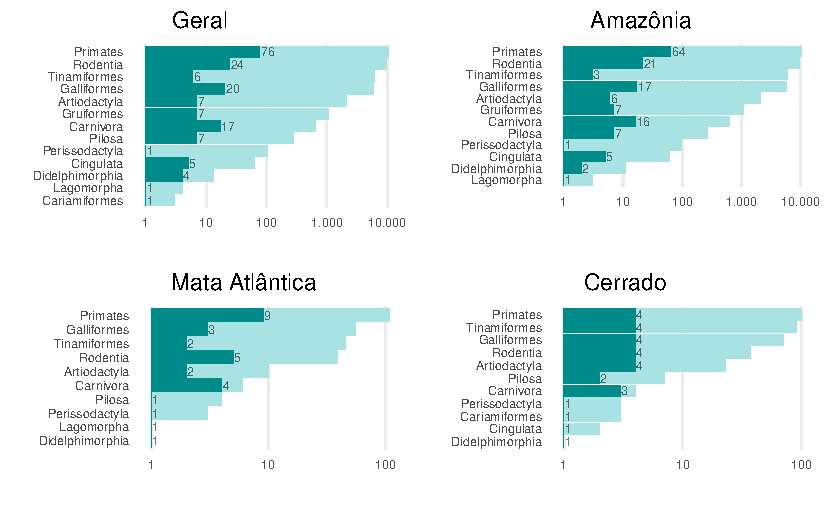
\includegraphics[width=0.85\textwidth,height=\textheight]{cap05_files/figure-pdf/fig-registros-ordem-1.pdf}

}

\caption{\label{fig-registros-ordem}Representatividade das principais
ordens de mamíferos amostradas no Programa Monitora, durante o período
de 2014 a 2022. As barras em verde escuro representam o número de
espécies registradas na ordem e a barras em verde claro o número de
registros naquela ordem.}

\end{figure}%

Em relação aos mamíferos, primatas foram o grupo preponderante. As cinco
famílias foram registradas e apenas o gênero \emph{Callibella} sp. não
foi observado. Setenta espécies diferentes foram registradas, o que
corresponde a 84,7\% do total de primatas brasileiros. Destas, 18
espécies são consideradas ameaçadas de extinção e duas possuem
deficiência de dados (DD) para avaliação.

Com relação as aves, até o momento, 38 táxons, entre gêneros e espécies,
foram registrados (Apêndice D). Durante as amostragens busca-se a
identificação no nível específico dos indivíduos observados, contudo, em
algumas unidades ocorrem em simpatria duas, três ou mais espécies de um
mesmo gênero, e, na maioria das vezes, essas espécies são semelhantes
entre si. Isso faz com que, por segurança, a validação desses registros
seja realizada no nível de gênero. São situações que podem ocorrer com
os gêneros \emph{Nothura} (codornas), \emph{Penelope} (jacus), Tinamus
(macucos) e \emph{Crypturellus} (inhambus), todos estes gêneros com um
ou mais táxons ameaçados de extinção (Apêndice D), conforme a Portaria
MMA nº 148/22.

A grande maioria dos registros de Aves está quase igualmente distribuída
entre Galliformes e Tinamídeos. Esse resultado se deve ao fato de a
detecção do método ser eficiente para o registro desses grupos, mas
também por Gruiformes (jacamins) ocorrerem apenas no bioma Amazônico, e
nunca com mais de uma espécie por localidade, enquanto que Cariamiformes
são típicos de ambientes abertos (fig-registros-ordem).

A variação entre as proporções de registros registadas para o Cerrado e
a Mata Atlântica ao longo dos nove anos de amostragem deve-se ao pequeno
número de unidades de conservação aderidas ao Programa Monitora, a
inconstância nas amostragens e ao pequeno esforço amostral, seja por
unidade de conservação, seja por bioma
(Figura~\ref{fig-registros-ordem}).

\subsection{Abundância relativa de mamíferos e aves por
biomas}\label{abunduxe2ncia-relativa-de-mamuxedferos-e-aves-por-biomas}

Em termos de abundância total de mamíferos e aves, o bioma Amazônico se
destaca em relação aos outros dois biomas tratados. Enquanto que Cerrado
e Mata Atlântica não parecem divergir de forma relevante
(Figura~\ref{fig-taxa-encontro-bioma}). O valor médio da abundância
relativa de mamíferos e aves no bioma Amazônia variou de ?? em 20?? a ??
avistamentos por 10 km percorridos em 20??, para mamíferos e ?? em 20??
a ?? em 20?? para aves.

\begin{figure}[H]

\centering{

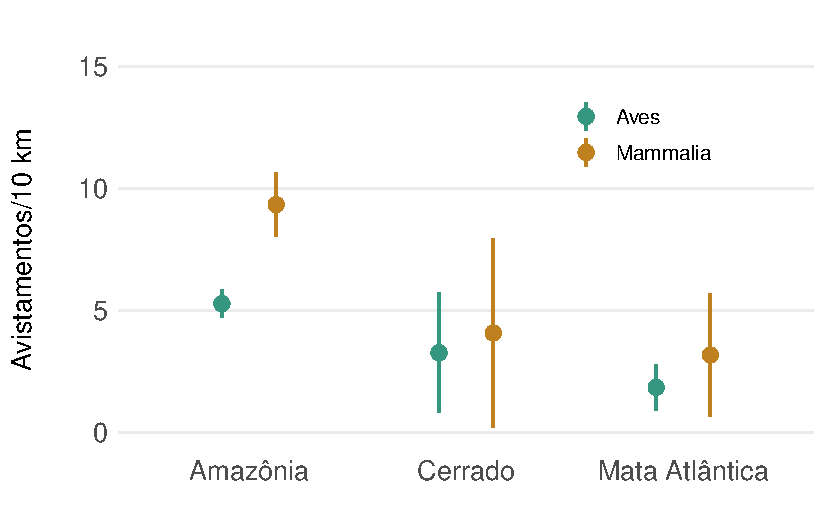
\includegraphics[width=0.7\textwidth,height=\textheight]{cap05_files/figure-pdf/fig-taxa-encontro-bioma-1.pdf}

}

\caption{\label{fig-taxa-encontro-bioma}Taxa de avistamento média de
aves e mamíferos por bioma para o período de 2014 a 2022.}

\end{figure}%

O valor médio da abundância relativa de mamíferos e aves no bioma
Amazônia variou de ?? em 20?? a ?? avistamentos por 10 km em 20??, para
mamíferos e de ?? em 20?? a ?? avistamentos por 10 km em 20??, para
aves. Quando se observa como essa abundância total de mamíferos e aves
variou entre os anos para os biomas
(Figura~\ref{fig-taxa-encontro-tempo}), verificamos que para a Amazônia
os primeiros anos apresentam uma maior dispersão dos resultados obtidos
explicada pelo proporcionalmente reduzido de UCs participantes e esforço
amostral, e um leve decréscimo nas abundâncias totais entre 2021 e 2022.
Para a Mata Atlântica os resultados não são consistentes devido a
descontinuidade de amostragem e variação no esforço entre os anos, já
para o Cerrado, o padrão observado se justifica\ldots xxxxxxxxx

\subsection{Taxa de encontro de mamíferos e aves ao longo do tempo -
geral e por bioma - 2014 a
2022}\label{taxa-de-encontro-de-mamuxedferos-e-aves-ao-longo-do-tempo---geral-e-por-bioma---2014-a-2022}

\begin{figure}[H]

\centering{

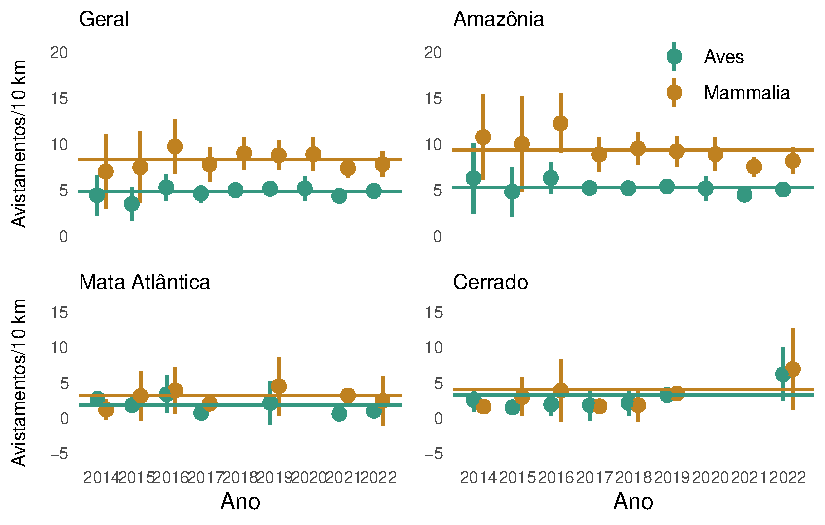
\includegraphics[width=0.85\textwidth,height=\textheight]{cap05_files/figure-pdf/fig-taxa-encontro-tempo-1.pdf}

}

\caption{\label{fig-taxa-encontro-tempo}Variação anual na taxa de
avistamento média de aves e mamíferos no período de 2014 a 2022 (geral e
por bioma). As linhas horizontais representam a taxa de avistamento
média para cada grupo considerando todo o período amostral.}

\end{figure}%

\subsection{Abundância de mamíferos e aves nas unidades de
conservação}\label{abunduxe2ncia-de-mamuxedferos-e-aves-nas-unidades-de-conservauxe7uxe3o}

Entre as UCs com maiores taxas totais para mamíferos encontramos a Rebio
do Uatumã, a Resex Verde para Sempre e a Esec da Terra do Meio
(Figura~\ref{fig-taxa-encontro-geral-mamiferos}), estas três UCs também
estão entre as quatro UCs com maiores taxas totais para aves
(Figura~\ref{fig-taxa-encontro-geral-aves}). Contudo, a posição da Resex
Verde para Sempre deve ser tomada com cautela visto que representa um
único ano de amostragem (2022). Uma visão espacial da taxa de
avistamento média geral, considerando conjuntamente aves e mamíferos, é
apresentada na figura Figura~\ref{fig-taxa-encontro-mapa}.

\begin{figure}[H]

\centering{

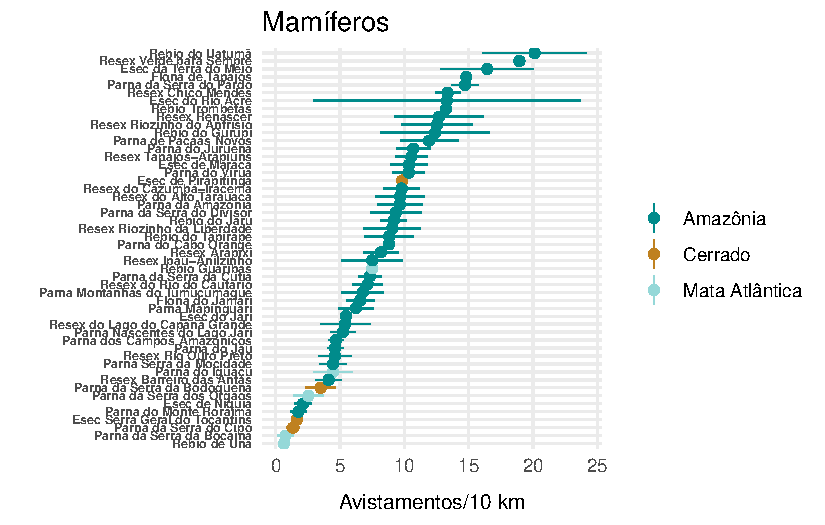
\includegraphics[width=0.7\textwidth,height=\textheight]{cap05_files/figure-pdf/fig-taxa-encontro-geral-mamiferos-1.pdf}

}

\caption{\label{fig-taxa-encontro-geral-mamiferos}Taxa média de
avistamento de aves por unidade de conservação, para o período de 2014 a
2022.}

\end{figure}%

\begin{figure}[H]

\centering{

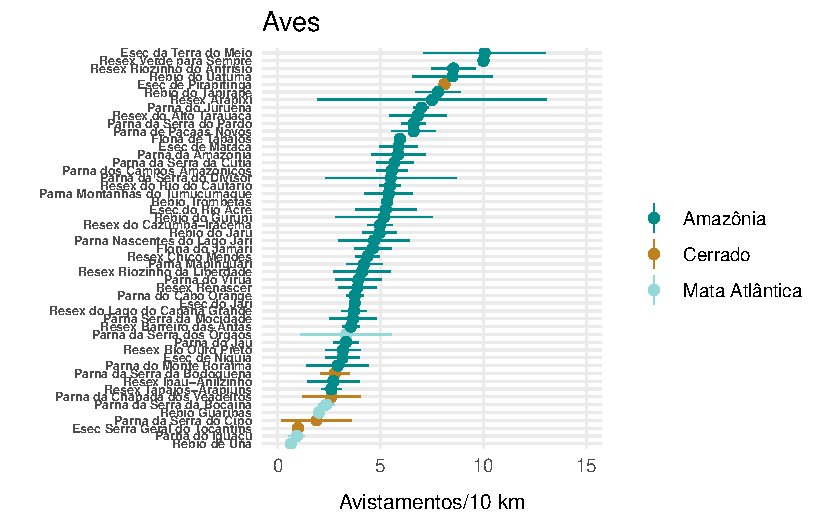
\includegraphics[width=0.7\textwidth,height=\textheight]{cap05_files/figure-pdf/fig-taxa-encontro-geral-aves-1.pdf}

}

\caption{\label{fig-taxa-encontro-geral-aves}Taxa média de avistamento
de aves por unidade de conservação, para o período de 2014 a 2022.}

\end{figure}%

\subparagraph{Variação espacial na taxa de encontro média - mamíferos e
aves
conjuntamente}\label{variauxe7uxe3o-espacial-na-taxa-de-encontro-muxe9dia---mamuxedferos-e-aves-conjuntamente}

\begin{figure}[H]

\centering{

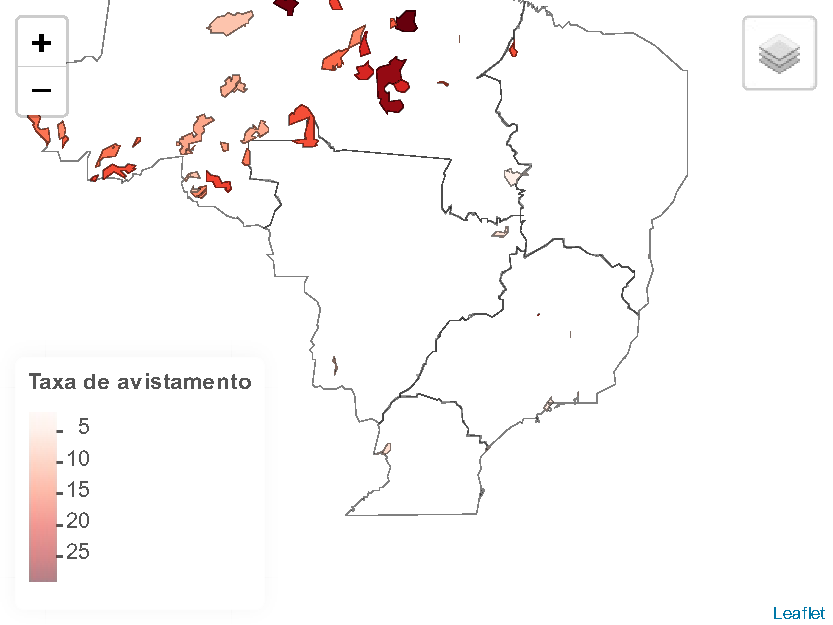
\includegraphics[width=0.7\textwidth,height=\textheight]{cap05_files/figure-pdf/fig-taxa-encontro-mapa-1.pdf}

}

\caption{\label{fig-taxa-encontro-mapa}Distribuição espacial das taxas
médias de avistamento de mamíferos e aves (taxa geral, consierando
conjuntamente os dois grupos) registradas nas unidades de conservação
integrantes do Programa Monitora de 2014 a 2022.}

\end{figure}%

\subsection{Considerações sobre algumas espécie
ameaçadas}\label{considerauxe7uxf5es-sobre-algumas-espuxe9cie-ameauxe7adas}

Dentre as espécies de aves alvo deste protocolo, quatorze espécies
ameaçadas ocorrem ou poderia ser esperado que ocorressem nas 52 unidades
de conservação analisadas. A saber, \emph{Nothura minor},
\emph{Taoniscus nanus}, \emph{Crypturellus zabele}, \emph{Tinamus tao},
\emph{Aburria jacutinga} e \emph{A. cujubi}, \emph{Penelope jacucaca} e
\emph{P. pileata}, \emph{Crax blumenbachii} e \emph{C. globulosa},
\emph{Psophia obscura}, \emph{P. interjecta}, \emph{P. viridis} e
\emph{P. dextralis}, mais duas subespécies, no caso \emph{Penelope s.
alagoensis} e \emph{Crax f.~pinima}.

Destes foram registrados \emph{Aburria cujubi}, \emph{Crax globulosa} e
as quatro espécies ameaçadas de \emph{Psophia}. Bem como, a subespécie
ameaçada de \emph{Penelope}). No entanto, ressaltamos que \emph{Tinamus
tao}, \emph{Penelope pileata}, \emph{P. jacucaca} e \emph{Nothura minor}
foram ou poderiam ter sido registrados em campo, porém, como ocorrem em
simpatria com espécies semelhantes, seus dados foram validados em nível
de gênero.

Importante ressaltar a ausência de registros de \emph{A. jacutinga}, que
seria esperada para quatro UCs na Mata Atlântica, na região Sul e
Sudeste, dada sua distribuição geográfica original.

\subsubsection{Abundância para algumas espécies ameaçadas de mamíferos e
aves}\label{abunduxe2ncia-para-algumas-espuxe9cies-ameauxe7adas-de-mamuxedferos-e-aves}

\begin{figure}[H]

\centering{

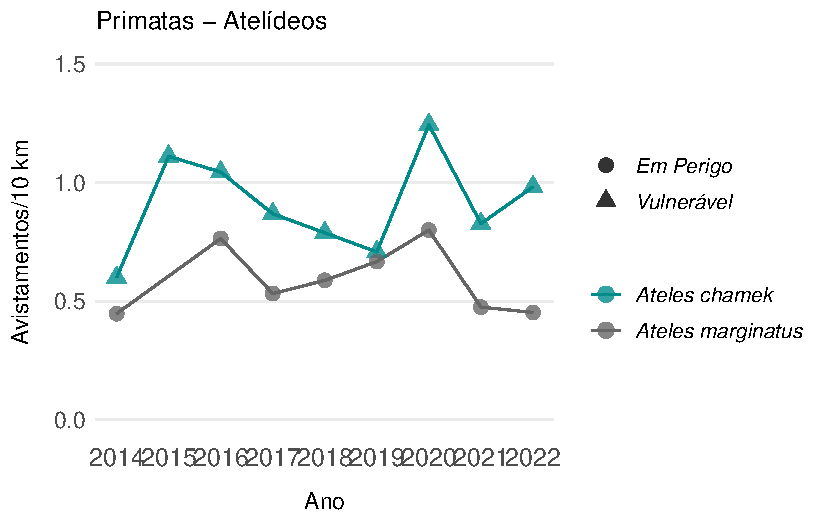
\includegraphics[width=0.7\textwidth,height=\textheight]{cap05_files/figure-pdf/fig-especies-ameacadas-atelideos-1.pdf}

}

\caption{\label{fig-especies-ameacadas-atelideos}Taxas médias de
avistamento estimadas por ano para duas espécies de primatas atelídeos
ameaçados. Os pontos representam valores médios obtidos a partir das
taxas registradas para diferentes unidades de conservação. As barras de
variação e o número de registros para cada ano não são apresentados para
maior clareza da figura.}

\end{figure}%

\begin{figure}[H]

\centering{

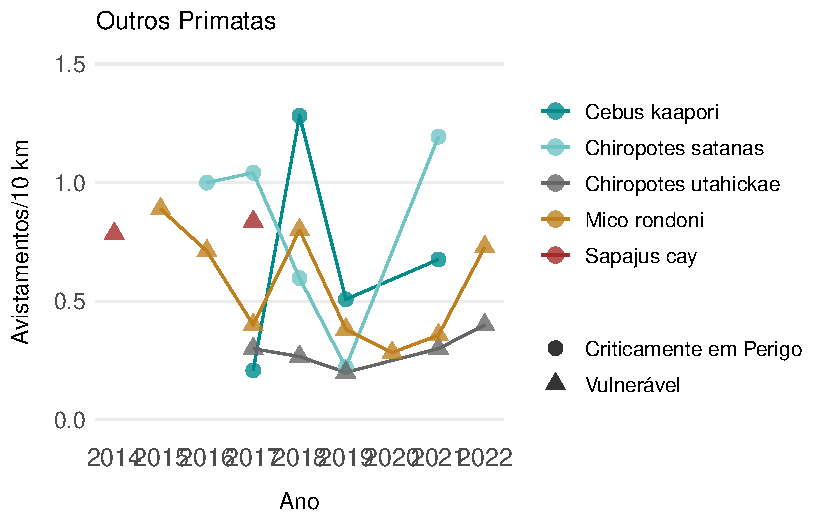
\includegraphics[width=0.7\textwidth,height=\textheight]{cap05_files/figure-pdf/fig-especies-ameacadas-outros-primatas-1.pdf}

}

\caption{\label{fig-especies-ameacadas-outros-primatas}Taxas médias de
avistamento estimadas por ano para cinco espécies de primatas ameaçados.
Os pontos representam valores médios obtidos a partir das taxas
registradas para diferentes unidades de conservação. As barras de
variação e o número de registros para cada ano não são apresentados para
maior clareza da figura.}

\end{figure}%

\begin{figure}[H]

\centering{

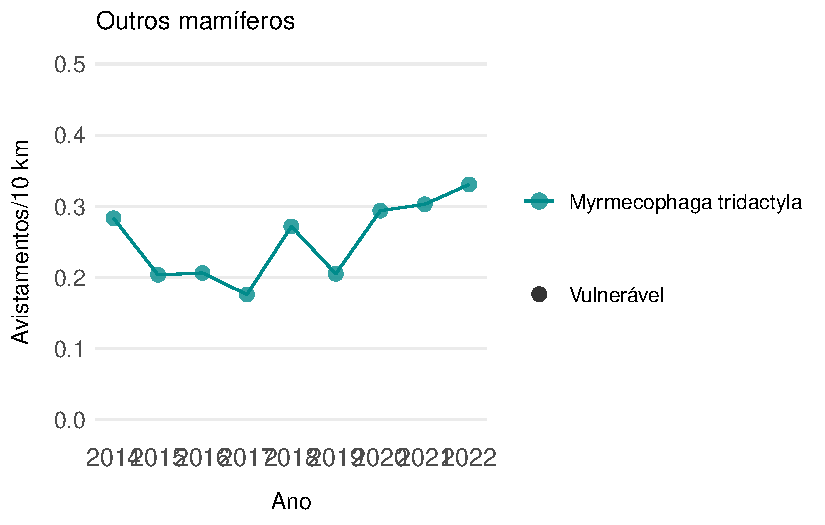
\includegraphics[width=0.7\textwidth,height=\textheight]{cap05_files/figure-pdf/fig-especies-ameacadas-tamandua-1.pdf}

}

\caption{\label{fig-especies-ameacadas-tamandua}Taxas médias de
avistamento estimadas por ano para a espécie ameaçada tamanduá-bandeira
(\emph{Myrmecophaga tridactyla}). Os pontos representam valores médios
obtidos a partir das taxas registradas para diferentes unidades de
conservação. As barras de variação e o número de registros para cada ano
não são apresentados para maior clareza da figura.}

\end{figure}%

\begin{figure}[H]

\centering{

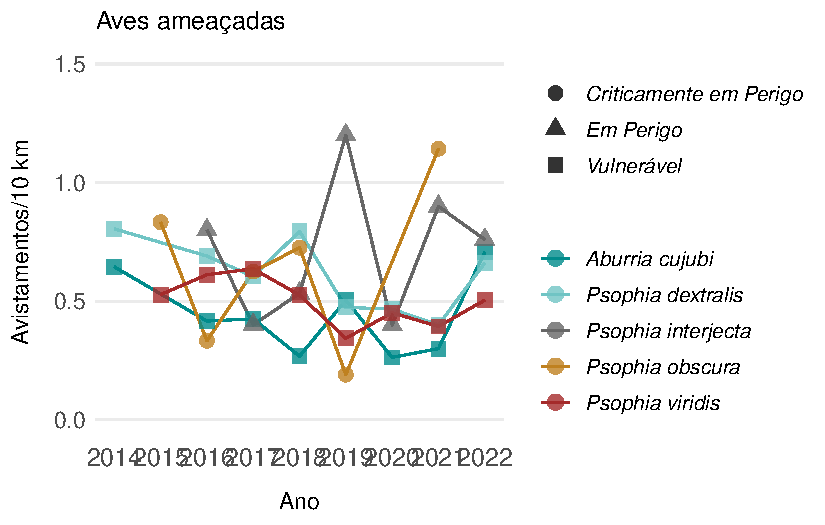
\includegraphics[width=0.7\textwidth,height=\textheight]{cap05_files/figure-pdf/fig-especies-ameacadas-aves-1.pdf}

}

\caption{\label{fig-especies-ameacadas-aves}Taxas médias de avistamento
estimadas por ano para cinco espécies de aves ameaçadas. Os pontos
representam valores médios obtidos a partir das taxas registradas para
diferentes unidades de conservação. As barras de variação e o número de
registros para cada ano não são apresentados para maior clareza da
figura.}

\end{figure}%

\subsection{Média Geométrica das populações (Living Planet Index --
LPI)}\label{muxe9dia-geomuxe9trica-das-populauxe7uxf5es-living-planet-index-lpi}

A média geométrica das abundâncias relativas é uma medida de escolha
para monitoramento de tendências da biodiversidade em diversos programas
(Buckland et al., 2005; {[}19{]}). Este índice reflete tendências na
abundância e equitabilidade entre as populações, e não é afetado pelo
ano base escolhido nem por variações inter-populacionais na
detectabilidade, por ser baseado em tendências intra-populacionais
({[}20{]}; {[}21{]}). Para o cálculo da média geométrica, utilizamos
dados de 160 populações em 22 UCs. Somente foram incluídas populações
com pelo menos cinco anos de monitoramento, taxa de encontro média
\textgreater{} 0.5 encontros a cada 10 km, e com esforço amostral
suficiente para atingir um coeficiente de variação da taxa de encontro ≥
0.25. A média geométrica e seu intervalo de confiança foram estimados
por bootstrap seguindo as recomendações de ({[}22{]}, {[}20{]}).

\subsubsection{Resultado da Média
Geométrica}\label{resultado-da-muxe9dia-geomuxe9trica}

A média geométrica das abundâncias relativas das populações analisadas
permaneceu estável ao longo do monitoramento, com o intervalo de 95\% de
credibilidade incluindo a linha de base durante todo o período
(Figura~\ref{fig-media-geometrica}). Esse resultado sugere que as UCs
monitoradas tem sido efetivas para a conservação das espécies de aves e
mamíferos alvo do Programa Monitora. Embora essa seja uma ótima notícia,
ela deve ser interpretada em seu devido contexto, em especial
considerando que o protocolo foca principalmente espécies relativamente
comuns e ecologicamente flexíveis, que a duração do monitoramento foi
relativamente curta em relação à longevidade das espécies-alvo, e que a
maioria das estações amostrais foi estabelecida em áreas de referência
(áreas íntegras no interior das UCs), representando cenários ideais e
não necessariamente os gradientes de pressão que atuam sobre a
biodiversidade na escala regional e/ou fora das UCs. A continuação do
monitoramento e o estabelecimento de estações amostrais em áreas
impactadas pode elucidar melhor as tendências da biodiversidade.

\begin{figure}[H]

\centering{

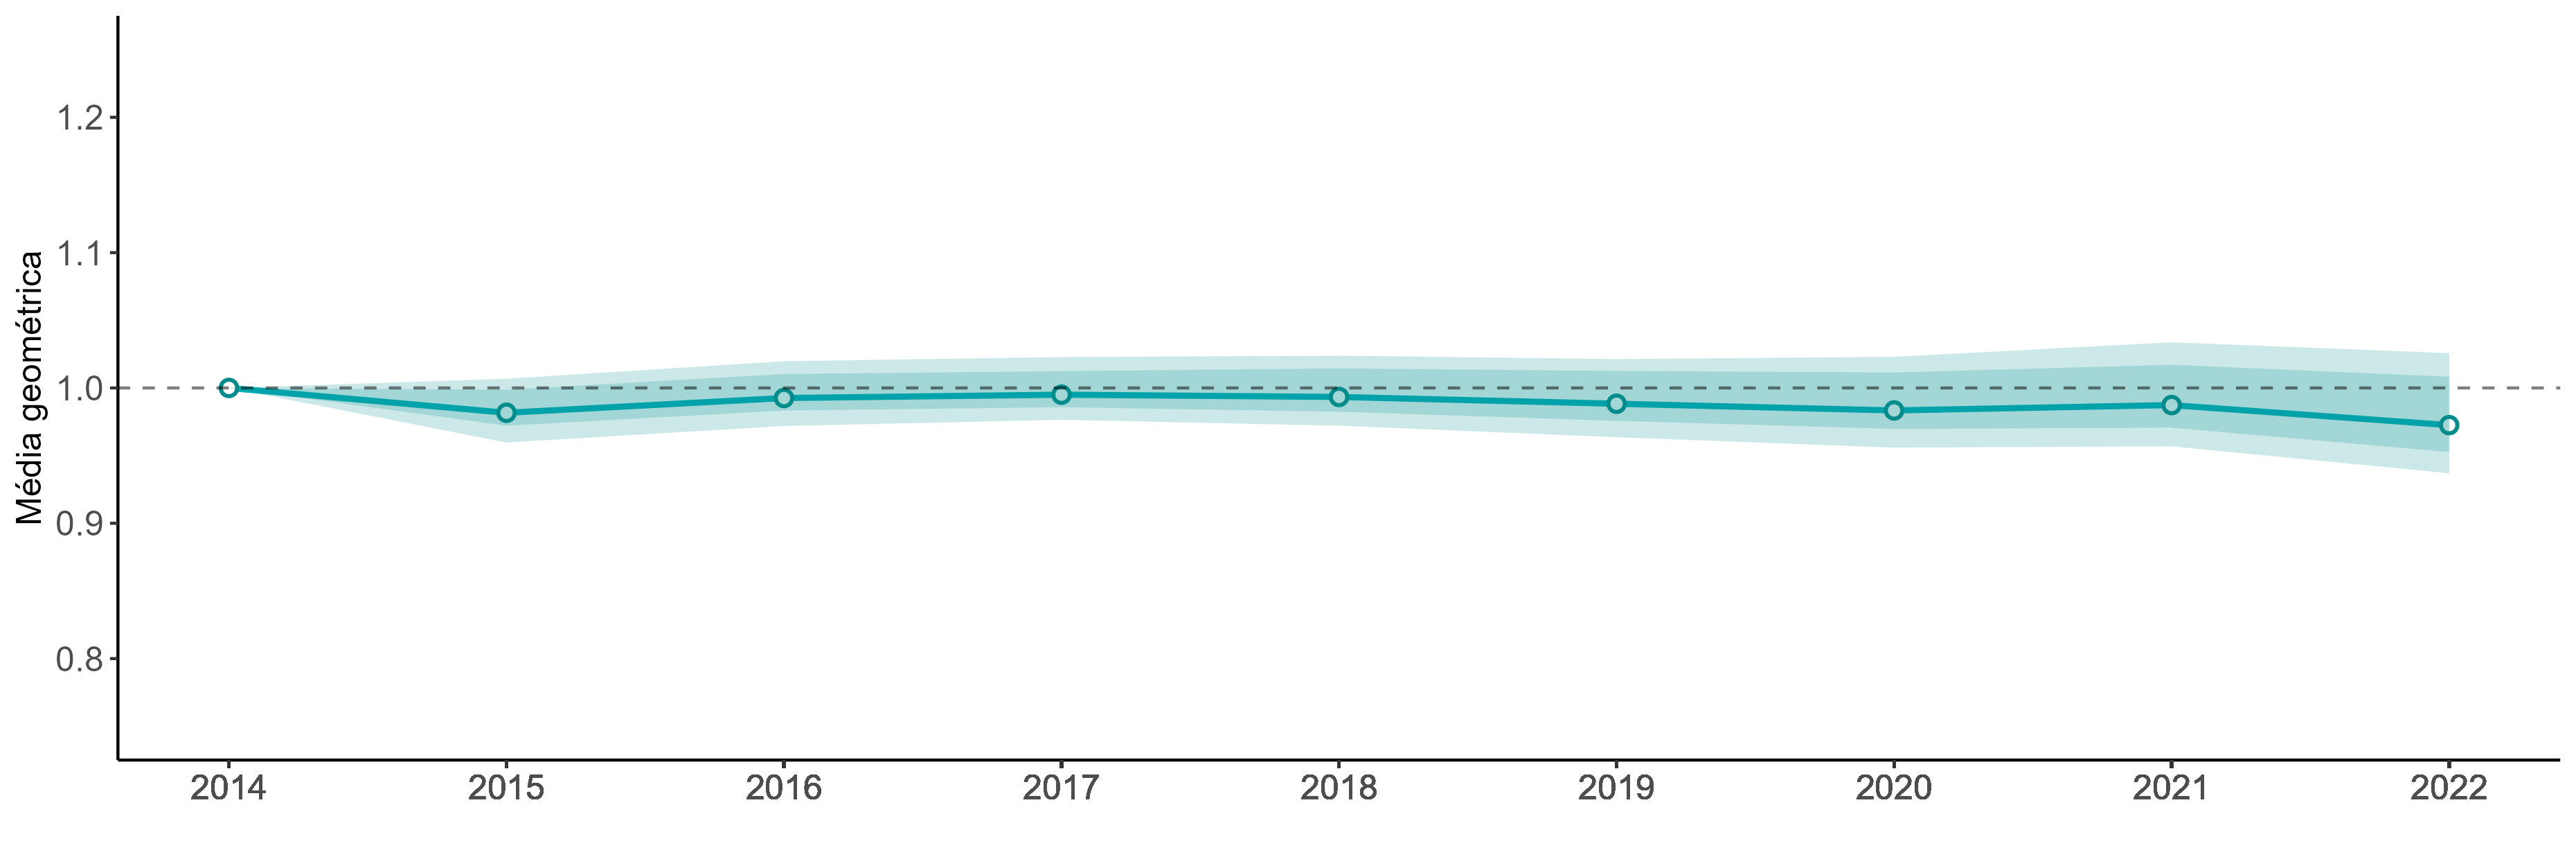
\includegraphics[width=0.7\textwidth,height=\textheight]{imagens/cap05/ma_media_geometrica.JPG}

}

\caption{\label{fig-media-geometrica}Média geométrica das estimativas de
abundãncia relativa para 160 populações monitoradas. A linha branca
escura corresponde aos valores médios; as faixas azuladasombreadas, ao
intervalo de confiança de 90 e 95\%.}

\end{figure}%

\section{Destaques}\label{destaques-2}

\emph{There are many variations of passages of Lorem Ipsum available,
but the majority have suffered alteration in some form, by injected
humour, or randomised words which don't look even slightly believable.
If you are going to use a passage of Lorem Ipsum, you need to be sure
there isn't anything embarrassing hidden in the middle of text. All the
Lorem Ipsum generators on the Internet tend to repeat predefined chunks
as necessary, making this the first true generator on the Internet. It
uses a dictionary of over 200 Latin words, combined with a handful of
model sentence structures, to generate Lorem Ipsum which looks
reasonable. The generated Lorem Ipsum is therefore always free from
repetition, injected humour, or non-characteristic words etc.}

\section{Discussão}\label{discussuxe3o-2}

\emph{There are many variations of passages of Lorem Ipsum available,
but the majority have suffered alteration in some form, by injected
humour, or randomised words which don't look even slightly believable.
If you are going to use a passage of Lorem Ipsum, you need to be sure
there isn't anything embarrassing hidden in the middle of text. All the
Lorem Ipsum generators on the Internet tend to repeat predefined chunks
as necessary, making this the first true generator on the Internet. It
uses a dictionary of over 200 Latin words, combined with a handful of
model sentence structures, to generate Lorem Ipsum which looks
reasonable. The generated Lorem Ipsum is therefore always free from
repetition, injected humour, or non-characteristic words etc.}

\section{Recomendações}\label{recomendauxe7uxf5es-2}

\emph{There are many variations of passages of Lorem Ipsum available,
but the majority have suffered alteration in some form, by injected
humour, or randomised words which don't look even slightly believable.
If you are going to use a passage of Lorem Ipsum, you need to be sure
there isn't anything embarrassing hidden in the middle of text. All the
Lorem Ipsum generators on the Internet tend to repeat predefined chunks
as necessary, making this the first true generator on the Internet. It
uses a dictionary of over 200 Latin words, combined with a handful of
model sentence structures, to generate Lorem Ipsum which looks
reasonable. The generated Lorem Ipsum is therefore always free from
repetition, injected humour, or non-characteristic words etc.}

\bookmarksetup{startatroot}

\chapter{Análise da correspondência e complementariedade dos
indicadores}\label{anuxe1lise-da-corresponduxeancia-e-complementariedade-dos-indicadores}

\emph{There are many variations of passages of Lorem Ipsum available,
but the majority have suffered alteration in some form, by injected
humour, or randomised words which don't look even slightly believable.
If you are going to use a passage of Lorem Ipsum, you need to be sure
there isn't anything embarrassing hidden in the middle of text. All the
Lorem Ipsum generators on the Internet tend to repeat predefined chunks
as necessary, making this the first true generator on the Internet. It
uses a dictionary of over 200 Latin words, combined with a handful of
model sentence structures, to generate Lorem Ipsum which looks
reasonable. The generated Lorem Ipsum is therefore always free from
repetition, injected humour, or non-characteristic words etc.}

\bookmarksetup{startatroot}

\chapter{Considerações finais}\label{cap7}

\emph{There are many variations of passages of Lorem Ipsum available,
but the majority have suffered alteration in some form, by injected
humour, or randomised words which don't look even slightly believable.
If you are going to use a passage of Lorem Ipsum, you need to be sure
there isn't anything embarrassing hidden in the middle of text. All the
Lorem Ipsum generators on the Internet tend to repeat predefined chunks
as necessary, making this the first true generator on the Internet. It
uses a dictionary of over 200 Latin words, combined with a handful of
model sentence structures, to generate Lorem Ipsum which looks
reasonable. The generated Lorem Ipsum is therefore always free from
repetition, injected humour, or non-characteristic words etc.}

\bookmarksetup{startatroot}

\chapter*{Referências bibliográficas}\label{referencias}
\addcontentsline{toc}{chapter}{Referências bibliográficas}

\markboth{Referências bibliográficas}{Referências bibliográficas}

\phantomsection\label{refs}
\begin{CSLReferences}{0}{1}
\bibitem[\citeproctext]{ref-Higuchi_1998}
\CSLLeftMargin{1. }%
\CSLRightInline{Higuchi N, Santos J dos, Ribeiro RJ, Minette L, Biot Y.
Biomassa da parte aérea da vegetação da floresta tropical úmida de
terra-firme da amazônia brasileira. Acta Amazonica. 1998;28: 153--153.
doi:\href{https://doi.org/10.1590/1809-43921998282166}{10.1590/1809-43921998282166}}

\bibitem[\citeproctext]{ref-Scolforo_2018}
\CSLLeftMargin{2. }%
\CSLRightInline{Scolforo JR, Rufini AL, Mello JM, Trugilho PF, Oliveira
AD, Silva CPC. Inventário florestal de MG: Equações de volume, peso de
matéria seca e carbono para diferentes fitofisionomias da flora nativa.
Lavras, MG: Universidade Federal de Lavras; 2018. pp. 103--114. }

\bibitem[\citeproctext]{ref-Rezende_2006}
\CSLLeftMargin{3. }%
\CSLRightInline{Rezende AV, Vale AT, Sanquetta CR, Figueiredo Filho A,
Felfili JM. Omparação de modelos matemáticos para estimativa do volume,
biomassa e estoque de carbono da vegetação lenhosa de um cerrado sensu
stricto em brasília, DF. Scientia Forestalis. 2006; 65--76. }

\bibitem[\citeproctext]{ref-Uehara_Prado_2006}
\CSLLeftMargin{4. }%
\CSLRightInline{Uehara‐Prado M, Brown KS, Freitas AVL. Species richness,
composition and abundance of fruit‐feeding butterflies in the brazilian
atlantic forest: Comparison between a fragmented and a continuous
landscape. Global Ecology and Biogeography. 2006;16: 43--54.
doi:\href{https://doi.org/10.1111/j.1466-8238.2006.00267.x}{10.1111/j.1466-8238.2006.00267.x}}

\bibitem[\citeproctext]{ref-Ribeiro_2010}
\CSLLeftMargin{5. }%
\CSLRightInline{Ribeiro DB, Prado PI, Brown Jr. KS, Freitas AVL.
Temporal diversity patterns and phenology in fruit‐feeding butterflies
in the atlantic forest. Biotropica. 2010;42: 710--716.
doi:\href{https://doi.org/10.1111/j.1744-7429.2010.00648.x}{10.1111/j.1744-7429.2010.00648.x}}

\bibitem[\citeproctext]{ref-Smilanich_2012}
\CSLLeftMargin{6. }%
\CSLRightInline{Smilanich AM, Dyer LA. Effects of banana plantation
pesticides on the immune response of lepidopteran larvae and their
parasitoid natural enemies. Insects. 2012;3: 616--628.
doi:\href{https://doi.org/10.3390/insects3030616}{10.3390/insects3030616}}

\bibitem[\citeproctext]{ref-Ndakidemi_2016}
\CSLLeftMargin{7. }%
\CSLRightInline{Ndakidemi B, Mtei K, Ndakidemi PA. Impacts of synthetic
and botanical pesticides on beneficial insects. Agricultural Sciences.
2016;07: 364--372.
doi:\href{https://doi.org/10.4236/as.2016.76038}{10.4236/as.2016.76038}}

\bibitem[\citeproctext]{ref-Devictor_2012}
\CSLLeftMargin{8. }%
\CSLRightInline{Devictor V, Swaay C van, Brereton T, Brotons L,
Chamberlain D, Heliölä J, et al. Differences in the climatic debts of
birds and butterflies at a continental scale. Nature Climate Change.
2012;2: 121--124.
doi:\href{https://doi.org/10.1038/nclimate1347}{10.1038/nclimate1347}}

\bibitem[\citeproctext]{ref-Santos_2017}
\CSLLeftMargin{9. }%
\CSLRightInline{Santos JP, Iserhard CA, Carreira JYO, Freitas AVL.
Monitoring fruit-feeding butterfly assemblages in two vertical strata in
seasonal atlantic forest: Temporal species turnover is lower in the
canopy. Journal of Tropical Ecology. 2017;33: 345--355.
doi:\href{https://doi.org/10.1017/s0266467417000323}{10.1017/s0266467417000323}}

\bibitem[\citeproctext]{ref-Bellaver_2012}
\CSLLeftMargin{10. }%
\CSLRightInline{Bellaver JMF. Efeito de borda e estrutura das
comunidades de borboletas frugívoras em fragmentos de mata paludosa na
planície costeira norte do rio grande do sul. Master's thesis,
Universidade Federal do Rio Grande do Sul. 2012. }

\bibitem[\citeproctext]{ref-DeVries_1987}
\CSLLeftMargin{11. }%
\CSLRightInline{DeVries PJ. The butterflies of costa rica and their
natural history, volume {I}. Princeton, NJ: Princeton University Press;
1987. }

\bibitem[\citeproctext]{ref-Pereira_2006}
\CSLLeftMargin{12. }%
\CSLRightInline{Pereira H, Davidcooper H. Towards the global monitoring
of biodiversity change. Trends in Ecology and Evolution. 2006;21:
123--129.
doi:\href{https://doi.org/10.1016/j.tree.2005.10.015}{10.1016/j.tree.2005.10.015}}

\bibitem[\citeproctext]{ref-WWF_2018}
\CSLLeftMargin{13. }%
\CSLRightInline{Grooten M, Almond REA(Eds). Living planet report 2018:
Aiming higher. Gland, Switzerland: WWF; 2018. Report No.: ISBN:
978-2-940529-90-2. }

\bibitem[\citeproctext]{ref-Checa_2009}
\CSLLeftMargin{14. }%
\CSLRightInline{Checa MF, Barragán A, Rodríguez J, Christman M. Temporal
abundance patterns of butterfly communities (lepidoptera: Nymphalidae)
in the ecuadorian amazonia and their relationship with climate. Annales
de la Société entomologique de France (NS). 2009;45: 470--486.
doi:\href{https://doi.org/10.1080/00379271.2009.10697630}{10.1080/00379271.2009.10697630}}

\bibitem[\citeproctext]{ref-Marengo_2001}
\CSLLeftMargin{15. }%
\CSLRightInline{Marengo JA, Liebmann B, Kousky VE, Filizola NP, C.
WainerI. Onset and end of the rainy season in the brazilian amazon
basin. Journal of Climate. 2001;14: 833--852. }

\bibitem[\citeproctext]{ref-Van_2019}
\CSLLeftMargin{16. }%
\CSLRightInline{Van Swaay CAM, Dennis EB, Schmucki R, Sevilleja C,
Balalaikins M, Botham M, et al. The EU butterfly indicator for grassland
species: 1990-2017: Technical report. Butterfly Conservation Europe \&
ABLE/eBMS; 2018 Jun. }

\bibitem[\citeproctext]{ref-Redford_1992}
\CSLLeftMargin{17. }%
\CSLRightInline{Redford KH. The empty forest. BioScience. 1992;42:
412--422. doi:\href{https://doi.org/10.2307/1311860}{10.2307/1311860}}

\bibitem[\citeproctext]{ref-SALVE_2024}
\CSLLeftMargin{18. }%
\CSLRightInline{Instituto Chico Mendes de Conservação da Biodiversidade
- ICMBio. Sistema de avaliação do risco de extinção da biodiversidade --
SALVE. \url{https://salve.icmbio.gov.br/\#/}; 2024. }

\bibitem[\citeproctext]{ref-Green_2019}
\CSLLeftMargin{19. }%
\CSLRightInline{Green EJ, McRae L, Freeman R, Harfoot MBJ, Hill SLL,
Baldwin-Cantello W, et al. Below the canopy: Global trends in forest
vertebrate populations and their drivers. 2019.
doi:\href{https://doi.org/10.7287/peerj.preprints.27882v1}{10.7287/peerj.preprints.27882v1}}

\bibitem[\citeproctext]{ref-Buckland_2011}
\CSLLeftMargin{20. }%
\CSLRightInline{Buckland ST, Studeny AC, Magurran AE, Illian JB, Newson
SE. The geometric mean of relative abundance indices: A biodiversity
measure with a difference. Ecosphere. 2011;2: art100.
doi:\href{https://doi.org/10.1890/es11-00186.1}{10.1890/es11-00186.1}}

\bibitem[\citeproctext]{ref-Van_Strien_2012}
\CSLLeftMargin{21. }%
\CSLRightInline{Van Strien MJ, Keller D, Holderegger R. A new analytical
approach to landscape genetic modelling: Least‐cost transect analysis
and linear mixed models. Molecular Ecology. 2012;21: 4010--4023.
doi:\href{https://doi.org/10.1111/j.1365-294x.2012.05687.x}{10.1111/j.1365-294x.2012.05687.x}}

\bibitem[\citeproctext]{ref-Buckland_2005}
\CSLLeftMargin{22. }%
\CSLRightInline{Buckland ST, Magurran AE, Green RE, Fewster RM.
Monitoring change in biodiversity through composite indices.
Philosophical Transactions of the Royal Society B: Biological Sciences.
2005;360: 243--254.
doi:\href{https://doi.org/10.1098/rstb.2004.1589}{10.1098/rstb.2004.1589}}

\end{CSLReferences}

\cleardoublepage
\phantomsection
\addcontentsline{toc}{part}{Apêndices}
\appendix

\chapter*{(APPENDIX) Apêndices}\label{apendice}
\addcontentsline{toc}{chapter}{(APPENDIX) Apêndices}

\markboth{(APPENDIX) Apêndices}{(APPENDIX) Apêndices}

\pagestyle{headings}

\section*{Apêndice A - Lista de
coletores}\label{apuxeandice-a---lista-de-coletores}
\addcontentsline{toc}{section}{Apêndice A - Lista de coletores}

\markright{Apêndice A - Lista de coletores}

\hspace{1.5cm}

\section*{Apêndice B - Evolução do estágio de implementação do
Programa}\label{apuxeandice-b---evoluuxe7uxe3o-do-estuxe1gio-de-implementauxe7uxe3o-do-programa}
\addcontentsline{toc}{section}{Apêndice B - Evolução do estágio de
implementação do Programa}

\markright{Apêndice B - Evolução do estágio de implementação do
Programa}

\hspace{1.5cm}

\section*{Apêndice C - Lista de
mamíferos}\label{apuxeandice-c---lista-de-mamuxedferos}
\addcontentsline{toc}{section}{Apêndice C - Lista de mamíferos}

\markright{Apêndice C - Lista de mamíferos}

\hspace{1.5cm}

\captionsetup{labelsep=none}

\begin{longtable}[t]{ll>{}l}

\caption{\label{tbl-lista-mamiferos}}

\tabularnewline

\toprule
Ordem & Família & Táxon\\
\midrule
\endfirsthead
\multicolumn{3}{@{}l}{\textit{(continuação)}}\\
\toprule
Ordem & Família & Táxon\\
\midrule
\endhead

\endfoot
\bottomrule
\endlastfoot
Didelphimorphia (01)  & Didelphidae (01)  & \em{Didelphis marsupialis }\\
Pilosa (05)  & Bradypodidae (01)  & \em{Bradypus variegatus }\\
 & Megalonychidae (01)  & \em{Choloepus didactylus }\\
 & Myrmecophagidae (03)  & \em{Myrmecophaga tridactyla (VU) }\\
 &  & \em{Tamandua tetradactyla }\\
\addlinespace
 &  & \em{Cyclopes didactylus* }\\
Cingulata (04)  & Dasypodidae (04)  & \em{Cabassous unicinctus }\\
 &  & \em{Dasypus novemcinctus }\\
 &  & \em{Dasypus kappleri* }\\
 &  & \em{Priodontes maximus (VU) }\\
\addlinespace
Primates (64)  & Callitrichidae (14)  & \em{Callimico goeldii }\\
 &  & \em{Callithrix aurita (EN) }\\
 &  & \em{Callithrix jacchus }\\
 &  & \em{Callithrix penicillata }\\
 &  & \em{Cebuella pygmaea* }\\
\addlinespace
 &  & \em{Mico argentatus }\\
 &  & \em{Mico emiliae }\\
 &  & \em{Mico humeralifer }\\
 &  & \em{Mico melanurus }\\
 &  & \em{Mico rondoni (VU) }\\
\addlinespace
 &  & \em{Saguinus imperator }\\
 &  & \em{Saguinus midas }\\
 &  & \em{Saguinus niger (VU) }\\
 &  & \em{Saguinus weddelli }\\
 & Aotidae (2)  & \em{Aotus nigriceps }\\
\addlinespace
 &  & \em{Aotus infulatus* }\\
 & Cebidae (14)  & \em{Cebus albifrons }\\
 &  & \em{Cebus kaapori* (CR) }\\
 &  & \em{Cebus olivaceus }\\
 &  & \em{Cebus unicolor }\\
\addlinespace
 &  & \em{Saimiri boliviensis }\\
 &  & \em{Saimiri cassiquiarensis }\\
 &  & \em{Saimiri collinsi }\\
 &  & \em{Saimiri macrodon* }\\
 &  & \em{Saimiri sciureus }\\
\addlinespace
 &  & \em{Saimiri ustus }\\
 &  & \em{Sapajus apella }\\
 &  & \em{Sapajus cay (VU) }\\
 &  & \em{Sapajus macrocephalus }\\
 &  & \em{Sapajus nigritus }\\
\addlinespace
 & Pitheciidae (19)  & \em{Cacajao melanocephalus }\\
 &  & \em{Callicebus baptista* }\\
 &  & \em{Callicebus bernhardi }\\
 &  & \em{Callicebus brunneus }\\
 &  & \em{Callicebus cinerascens }\\
\addlinespace
 &  & \em{Callicebus cupreus }\\
 &  & \em{Callicebus dubius* }\\
 &  & \em{Callicebus hoffmannsi }\\
 &  & \em{Callicebus lugens* }\\
 &  & \em{Callicebus moloch }\\
\addlinespace
 &  & \em{Callicebus vieirai (DD) }\\
 &  & \em{Chiropotes albinasus }\\
 &  & \em{Chiropotes chiropotes* }\\
 &  & \em{Chiropotes sagulatus }\\
 &  & \em{Chiropotes satanas (CR) }\\
\addlinespace
 &  & \em{Chiropotes utahickae* }\\
 &  & \em{Pithecia irrorata (DD) }\\
 &  & \em{Pithecia monachus* }\\
 &  & \em{Pithecia pithecia }\\
 & Atelidae (15)  & \em{Alouatta belzebul (VU) }\\
\addlinespace
 &  & \em{Alouatta caraya }\\
 &  & \em{Alouatta discolor (VU) }\\
 &  & \em{Alouatta guariba clamitans }\\
 &  & \em{(VU) }\\
 &  & \em{Alouatta juara }\\
\addlinespace
 &  & \em{Alouatta macconnelli }\\
 &  & \em{Alouatta nigerrima }\\
 &  & \em{Alouatta puruensis }\\
 &  & \em{Ateles belzebuth* (VU) }\\
 &  & \em{Ateles chamek (VU) }\\
\addlinespace
 &  & \em{Ateles marginatus (EN) }\\
 &  & \em{Ateles paniscus }\\
 &  & \em{Brachyteles arachnoides (EN) }\\
 &  & \em{Lagothrix cana cana (EN) }\\
 &  & \em{Lagothrix poeppigii* (VU) }\\
\addlinespace
Carnivora (14)  & Canidae (3)  & \em{Atelocynus microtis* (VU) }\\
 &  & \em{Canis familiaris }\\
 &  & \em{Cerdocyon thous* }\\
 & Felidae (6)  & \em{Leopardus pardalis }\\
 &  & \em{Leopardus tigrinus (EN) }\\
\addlinespace
 &  & \em{Leopardus wiedii (VU) }\\
 &  & \em{Panthera onca (VU) }\\
 &  & \em{Puma concolor (VU) }\\
 &  & \em{Puma yagouaroundi (VU) }\\
 & Mustelidae (4)  & \em{Eira barbara }\\
\addlinespace
 &  & \em{Galictis vittata }\\
 &  & \em{Lontra longicaudis }\\
 &  & \em{Pteronura brasiliensis* (VU) }\\
 & Procyonidae (1)  & \em{Nasua nasua }\\
Artiodactyla (06)  & Cervidae (4)  & \em{Mazama americana (DD) }\\
\addlinespace
 &  & \em{Mazama gouazoubira }\\
 &  & \em{Mazama nemorivaga (DD) }\\
 &  & \em{Ozotocerus bezoarticus* (VU) }\\
 & Tayassuidae (2)  & \em{Pecari tajacu }\\
 &  & \em{Tayassu pecari (VU) }\\
\addlinespace
Perissodactyla (01)  & Tapiridae (1)  & \em{Tapirus terrestris (VU) }\\
Rodentia (20)  & Erethizontidae (2)  & \em{Coendou bicolor* }\\
 &  & \em{Coendou prehensilis* }\\
 & Cuniculidae (1)  & \em{Cuniculus paca }\\
 & Caviidae (1)  & \em{Hydrochoeris hydrochaeris* }\\
\addlinespace
 & Dasyproctidae (8)  & \em{Dasyprocta azarae }\\
 &  & \em{Dasyprocta croconota }\\
 &  & \em{Dasyprocta fuliginosa }\\
 &  & \em{Dasyprocta iacki }\\
 &  & \em{Dasyprocta leporina }\\
\addlinespace
 &  & \em{Dasyprocta prymnolopha }\\
 &  & \em{Myoprocta acouchy }\\
 &  & \em{Myoprocta pratti }\\
 & Sciuridae (8)  & \em{Guerlinguetus aestuans }\\
 &  & \em{Guerlinguetus gilvigularis* }\\
\addlinespace
 &  & \em{Guerlinguetus ignitus }\\
 &  & \em{Guerlinguetus ingrami }\\
 &  & \em{Microsciurus flaviventer }\\
 &  & \em{Sciurillus pusillus }\\
 &  & \em{Urosciurus igniventris }\\
\addlinespace
 &  & \em{Urosciurus spadiceus }\\
Lagomorpha (01)  & Leporidae (1)  & \em{Sylvilagus brasiliensis* }\\*

\end{longtable}

\section*{Apêndice D - Lista de
aves}\label{apuxeandice-d---lista-de-aves}
\addcontentsline{toc}{section}{Apêndice D - Lista de aves}

\markright{Apêndice D - Lista de aves}

\captionsetup{labelsep=none}

\begin{longtable}[t]{ll>{}l}

\caption{\label{tbl-lista-aves}}

\tabularnewline

\toprule
Ordem & Família & Táxon\\
\midrule
\endfirsthead
\multicolumn{3}{@{}l}{\textit{(continuação)}}\\
\toprule
Ordem & Família & Táxon\\
\midrule
\endhead

\endfoot
\bottomrule
\endlastfoot
Cariamiformes  & Cariamidae  & \em{Cariama cristata }\\
Tinamiformes  & Tinamidae  & \em{Crypturellus sp. (cerca 12 spp.) }\\
 &  & \em{Nothura sp. (N. Maculosa ou N. minor*) }\\
 &  & \em{Rhynchotus rufescens }\\
 &  & \em{Tinamus major }\\
\addlinespace
 &  & \em{Tinamus solitarius }\\
 &  & \em{Tinamus sp. (T. Guttatus, T. major  ou T. tao*) }\\
Galliformes  & Cracidae  & \em{Aburria cujubi* }\\
 &  & \em{Aburria cumanensis }\\
 &  & \em{Aburria sp. (A. Cumanensis ou A. cujubi*) }\\
\addlinespace
 &  & \em{Crax alector }\\
 &  & \em{Crax fasciolata }\\
 &  & \em{Crax globulosa* }\\
 &  & \em{Crax sp. (à confirmar) }\\
 &  & \em{Nothocrax urumutum }\\
\addlinespace
 &  & \em{Ortalis guttata }\\
 &  & \em{Ortalis motmot }\\
 &  & \em{Ortalis ruficeps }\\
 &  & \em{Ortalis superciliaris }\\
 &  & \em{Pauxi tomentosa }\\
\addlinespace
 &  & \em{Pauxi tuberosa }\\
 &  & \em{Pauxi sp. (P. tomentosa, P. tuberosa) }\\
 &  & \em{Penelope jacquacu }\\
 &  & \em{Penelope marail }\\
 &  & \em{Penelope obscura }\\
\addlinespace
 &  & \em{Penelope superciliaris alagoensis* }\\
 &  & \em{Penelope sp. (Penelope pileata*, P. jacucaca*, P. superciliaris ou P. ochrogaster) }\\
 & Odontophoridae  & \em{Odontophorus capueira }\\
 &  & \em{Odontophorus gujanensis }\\
 &  & \em{Odontophorus stellatus }\\
\addlinespace
 &  & \em{Odontophorus sp. (O. gujanensis, O. stellatus) }\\
Gruiformes  & Psophiidae  & \em{Psophia crepitans }\\
 &  & \em{Psophia dextralis* }\\
 &  & \em{Psophia interjecta* }\\
 &  & \em{Psophia leucoptera }\\
\addlinespace
 &  & \em{Psophia obscura* }\\
 &  & \em{Psophia ochroptera }\\
 &  & \em{Psophia viridis* }\\*

\end{longtable}


\backmatter

\end{document}
